% Biên dịch bằng XeLaTeX.
\documentclass[12pt,a4paper,oneside]{extreport}
\usepackage[left=3.1cm,right=2.1cm,top=2.4cm,bottom=2.3cm]{geometry}
\usepackage{fontspec}
\usepackage{amsmath}
\usepackage{unicode-math}
\IfFontExistsTF{Times New Roman}
  {\setmainfont{Times New Roman}}
  {\IfFontExistsTF{Liberation Serif}{\setmainfont{Liberation Serif}}{\setmainfont{TeX Gyre Termes}}}
\IfFontExistsTF{Liberation Mono}
  {\setmonofont{Liberation Mono}[Scale=MatchLowercase]}
  {\setmonofont{Latin Modern Mono}[Scale=MatchLowercase]}
\setmathfont{Latin Modern Math}
\usepackage{graphicx}
\usepackage{float}
\usepackage{caption}
\usepackage{array,longtable,booktabs}
\usepackage{calc}
\usepackage{fvextra}
\usepackage{setspace}
\usepackage{titlesec}
\usepackage[nottoc]{tocbibind}
\usepackage{xurl}
\usepackage{bookmark}
\usepackage{hyperref}
\hypersetup{hidelinks,plainpages=false,pageanchor=false,pdfauthor={Nguyễn Trung Nghĩa},
  pdftitle={Nghiên cứu mở rộng công cụ USE hỗ trợ đặc tả và kiểm chứng hệ thống đa tác tử}}
\urlstyle{same}

\renewcommand{\chaptername}{CHƯƠNG}
\renewcommand{\contentsname}{MỤC LỤC}
\renewcommand{\listfigurename}{DANH MỤC HÌNH}
\renewcommand{\listtablename}{DANH MỤC BẢNG}
\renewcommand{\figurename}{Hình}
\renewcommand{\tablename}{Bảng}
\renewcommand{\bibname}{TÀI LIỆU THAM KHẢO}
\titleformat{\chapter}[block]{\normalfont\centering\Large\bfseries}
  {\chaptername\ \thechapter.}{0.55em}{}
\titlespacing*{\chapter}{0pt}{0pt}{18pt}
\titlespacing*{\section}{0pt}{2ex plus .4ex}{.8ex}
\titlespacing*{\subsection}{0pt}{1.6ex plus .3ex}{.7ex}
\setcounter{secnumdepth}{2}
\setcounter{tocdepth}{2}
\setlength{\parindent}{0.75cm}
\setlength{\parskip}{3pt plus 1pt}
\setstretch{1.30}
\clubpenalty=10000
\widowpenalty=10000
\emergencystretch=2em

\floatplacement{figure}{H}
\captionsetup{font=small,labelfont=bf,labelsep=space,justification=centering}
\captionsetup[table]{position=top}
\DeclareRobustCommand{\thesisfigure}[1]{Hình~\ref{#1}}
\DeclareRobustCommand{\thesistable}[1]{Bảng~\ref{#1}}
\newcommand{\thesisdisplaytitle}[2]{%
  \par\smallskip\noindent\makebox[\linewidth][c]{\small\textbf{#1}\ #2}\par\nobreak}
\providecommand{\ul}[1]{\underline{#1}}
\providecommand{\tightlist}{\setlength{\itemsep}{0pt}\setlength{\parskip}{0pt}}
\fvset{breaklines=true,breakanywhere=true,fontsize=\small}
\setkeys{Gin}{keepaspectratio}

\begin{document}
\begin{titlepage}
\centering

\vspace*{0.20cm}
{\large\bfseries

ĐẠI HỌC QUỐC GIA HÀ NỘI

TRƯỜNG ĐẠI HỌC CÔNG NGHỆ

\par}

\vspace{1cm}


\includegraphics[width=1.2008in,height=\textheight]{figures/logo.png}

\vspace{0.65cm}

Nguyễn Trung Nghĩa

\vspace{0.85cm}
{\Large\bfseries

NGHIÊN CỨU MỞ RỘNG CÔNG CỤ USE HỖ TRỢ ĐẶC TẢ VÀ KIỂM CHỨNG HỆ THỐNG ĐA TÁC TỬ

\par}

\vspace{0.95cm}
{\large\bfseries

KHÓA LUẬN TỐT NGHIỆP HỆ CHÍNH QUY

\par}

\vspace{0.30cm}

Ngành: Công nghệ thông tin

\vfill

HÀ NỘI - 2026

\end{titlepage}

\begin{titlepage}
\centering

\vspace*{0.20cm}
{\large\bfseries

ĐẠI HỌC QUỐC GIA HÀ NỘI

TRƯỜNG ĐẠI HỌC CÔNG NGHỆ

\par}

\vspace{2.0cm}

Nguyễn Trung Nghĩa

\vspace{0.85cm}
{\Large\bfseries

NGHIÊN CỨU MỞ RỘNG CÔNG CỤ USE HỖ TRỢ ĐẶC TẢ VÀ KIỂM CHỨNG HỆ THỐNG ĐA TÁC TỬ

\par}

\vspace{0.95cm}
{\large\bfseries

KHÓA LUẬN TỐT NGHIỆP HỆ CHÍNH QUY

\par}

\vspace{0.30cm}

Ngành: Công nghệ thông tin

Cán bộ hướng dẫn: PGS. TS. Đặng Đức Hạnh

\vfill

HÀ NỘI - 2026

\end{titlepage}

\clearpage
\pagenumbering{roman}
\hypersetup{pageanchor=true}

\chapter*{TÓM TẮT}

Trong các hệ thống đa tác tử, nhiều tác tử hoạt động tự chủ và phối hợp để thực hiện các mục tiêu chung. Tuy nhiên, sự tương tác giữa các tác tử khiến việc xác định tính đúng đắn của hệ thống và mức độ đạt được các mục tiêu trở nên phức tạp. Các phương pháp đặc tả và kiểm chứng dựa trên mô hình, kết hợp với ngôn ngữ ràng buộc OCL, cung cấp cơ sở để đánh giá tính hợp lệ của trạng thái hệ thống. Bên cạnh đó, mô hình iStar hỗ trợ biểu diễn và phân tích các mục tiêu, nhiệm vụ cùng mối quan hệ giữa chúng. Tuy nhiên, thách thức đặt ra là làm thế nào để kết nối các mô hình đặc tả với trạng thái thực tế của hệ thống đa tác tử trong quá trình thực thi. Nghiên cứu này mở rộng công cụ USE để hỗ trợ đặc tả và kiểm chứng hệ thống đa tác tử xây dựng trên JaCaMo. Phương pháp sử dụng CSL để mô tả cấu trúc và ràng buộc, kết hợp iStar để đánh giá tiến độ thực hiện mục tiêu và nhiệm vụ. Thông qua cơ chế thu thập, ánh xạ và kiểm chứng trạng thái tại các điểm kiểm tra trong quá trình thực thi, nghiên cứu hướng tới hỗ trợ phát hiện vi phạm và theo dõi mức độ đạt mục tiêu, góp phần nâng cao khả năng kiểm soát và đánh giá hệ thống đa tác tử.

\emph{Từ khóa: JaCaMo, USE, CSL, iStar, kiểm chứng hệ thống đa tác tử.}

\chapter*{LỜI CAM ĐOAN}

Em là Nguyễn Trung Nghĩa, sinh viên khóa QH-2023-K68I-IT20, Trường Đại học Công nghệ -- Đại học Quốc gia Hà Nội, xin cam đoan khóa luận tốt nghiệp ``Nghiên cứu mở rộng công cụ USE hỗ trợ đặc tả và kiểm chứng hệ thống đa tác tử'' là công trình do em tự thực hiện dưới sự đầu tư nghiên cứu nghiêm túc của bản thân và sự hướng dẫn tận tình của PGS. TS. Đặng Đức Hạnh cùng anh Nguyễn Đức Quyền.

Tất cả các tài liệu tham khảo đều được em trích dẫn và ghi rõ nguồn gốc, không có hành vi sao chép tài liệu hay công trình nghiên cứu của người khác. Nếu phát hiện bất kỳ sai phạm nào, em xin chịu hoàn toàn trách nhiệm trước Hội đồng kỷ luật Khoa Công nghệ Thông tin và Trường Đại học Công nghệ -- Đại học Quốc gia Hà Nội.

Bên cạnh đó, trong quá trình nghiên cứu, phát triển hệ thống và hoàn thiện khóa luận, em có sử dụng một số công cụ trí tuệ nhân tạo (AI) như ChatGPT, Gemini nhằm hỗ trợ tìm hiểu kiến thức, tham khảo ý tưởng, phân tích và phát triển mã nguồn, kiểm tra lỗi cũng như cải thiện cách diễn đạt. Tuy nhiên, các công cụ này chỉ đóng vai trò hỗ trợ; em trực tiếp xem xét, đánh giá và kiểm chứng các nội dung, giải pháp và kết quả được sử dụng trong khóa luận, đồng thời chịu trách nhiệm về tính chính xác, trung thực của toàn bộ công trình nghiên cứu.

\emph{Hà Nội, ngày .\ldots. tháng 12 năm 2026}

\textbf{Sinh viên}

\textbf{NGUYỄN TRUNG NGHĨA}

\chapter*{LỜI CẢM ƠN}

Trước hết, em xin bày tỏ lòng biết ơn sâu sắc đến PGS. TS. Đặng Đức Hạnh, người thầy đã tận tình hướng dẫn và định hướng cho em trong suốt quá trình nghiên cứu và thực hiện khóa luận tốt nghiệp. Những kiến thức chuyên môn, kinh nghiệm cùng những lời góp ý quý báu của thầy đã giúp em nâng cao tư duy khoa học, khả năng phân tích và tiếp cận vấn đề một cách chặt chẽ. Sự tận tâm và nhiệt huyết của thầy là nguồn động lực lớn lao giúp em không ngừng học hỏi và hoàn thiện bản thân.

Em xin gửi lời cảm ơn đặc biệt đến anh Nguyễn Đức Quyền, người đã luôn đồng hành và trực tiếp hỗ trợ em trong quá trình thực hiện đề tài. Anh đã dành nhiều thời gian chia sẻ kiến thức, giải đáp thắc mắc và tận tình hướng dẫn em vượt qua những khó khăn trong quá trình nghiên cứu và phát triển hệ thống. Những góp ý, định hướng cùng kinh nghiệm quý báu của anh không chỉ giúp em từng bước hoàn thiện khóa luận mà còn giúp em học hỏi được nhiều điều về tư duy nghiên cứu và cách giải quyết vấn đề. Em thực sự trân trọng sự nhiệt tình, kiên nhẫn và những tâm huyết mà anh đã dành cho em trong suốt thời gian qua.

Bên cạnh đó, em xin chân thành cảm ơn các thầy cô, anh chị và các bạn trong nhóm nghiên cứu SME Lab đã luôn chia sẻ kiến thức, kinh nghiệm và tạo nên một môi trường học tập, nghiên cứu tích cực. Sự hỗ trợ và những đóng góp của mọi người đã giúp em mở rộng hiểu biết và có thêm nhiều kinh nghiệm quý báu.

Em cũng xin dành lời tri ân sâu sắc đến gia đình, những người đã luôn yêu thương, động viên và tạo mọi điều kiện thuận lợi để em yên tâm học tập, nghiên cứu và hoàn thành khóa luận.

Cuối cùng, em xin gửi lời cảm ơn đến Trường Đại học Công nghệ -- Đại học Quốc gia Hà Nội đã tạo điều kiện để em được học tập, nghiên cứu và thực hiện đề tài ``Nghiên cứu mở rộng công cụ USE hỗ trợ đặc tả và kiểm chứng hệ thống đa tác tử''. Đây là cơ hội quý báu để em vận dụng kiến thức đã học, tiếp cận những vấn đề chuyên sâu và tích lũy kinh nghiệm cho chặng đường phát triển sau này.

Em xin chân thành cảm ơn tất cả những người đã luôn đồng hành, giúp đỡ và động viên em trong suốt quá trình thực hiện khóa luận tốt nghiệp.

\emph{Hà Nội, ngày .\ldots. tháng 12 năm 2026}

\textbf{Sinh viên}

\textbf{NGUYỄN TRUNG NGHĨA}

\tableofcontents
\listoffigures
\listoftables

\chapter*{MỞ ĐẦU}\label{mo-dau}
\addcontentsline{toc}{chapter}{MỞ ĐẦU}

Trong hệ thống đa tác tử, các tác tử tự chủ phối hợp để thực hiện công việc chung~\cite{ref-1}. JaCaMo là nền tảng lập trình cho các hệ thống này, kết hợp tác tử, môi trường dùng chung và tổ chức phân vai~\cite{ref-2}. Khi kết quả của một bên là đầu vào của bên khác, cách phối hợp ảnh hưởng trực tiếp đến tiến độ chung.

Khi các hành động xen kẽ, một tác tử có thể làm thay đổi dữ liệu mà tác tử khác đang dùng. Trạng thái có thể thỏa quy tắc nghiệp vụ dù một nhiệm vụ còn dang dở. Việc đánh giá tiến độ vì vậy cần xét cả trạng thái hiện tại và diễn biến trước đó~\cite{ref-5}.

RV4JaCa kiểm chứng giao thức JaCaMo qua thông điệp khi hệ thống chạy~\cite{ref-24}. USE kiểm tra bất biến OCL trên trạng thái đối tượng~\cite{ref-4}, còn iStar mô tả mục tiêu và nhiệm vụ~\cite{ref-12}. Để đánh giá cả ràng buộc lẫn tiến độ trong cùng một lần chạy, cần dựng trạng thái từ dữ liệu JaCaMo và giữ lịch sử riêng của từng đối tượng.

Nghiên cứu mở rộng USE để kiểm chứng JaCaMo khi thực thi, kế thừa CSL (Composite State Language) và cách gắn điều kiện vào iStar từ công trình về sự phù hợp giữa iStar và BPMN~\cite{ref-28}. Tại mỗi checkpoint, plugin dựng trạng thái CSL từ ảnh chụp JaCaMo. USE kiểm tra bất biến OCL, cập nhật Goal và Task theo lịch sử rồi trả quyết định tiếp tục hoặc giữ dừng.

Thực nghiệm cho thấy công cụ giữ lịch sử riêng cho hai phiên Auction và phân biệt vi phạm với trường hợp thiếu dữ liệu. Khi đánh giá lại cùng một vết Auction với cùng đặc tả, các quyết định và tập mục tiêu, nhiệm vụ đã đạt đều khớp ở cả 58 checkpoint (Mục 3.5).

Các đóng góp gồm phép ánh xạ bảo toàn định danh, bộ đánh giá theo lịch sử và cơ chế phản hồi tại checkpoint. Nghiên cứu trả lời ba câu hỏi.

\begin{enumerate}
\def\labelenumi{\roman{enumi})}
\item
  Làm thế nào để ánh xạ dữ liệu JaCaMo sang CSL và giữ định danh, lịch sử của từng đối tượng?
\item
  Làm thế nào để tổng hợp kết quả OCL và iStar tại checkpoint, đồng thời phân biệt vi phạm với thiếu dữ liệu?
\item
  Đánh giá lại cùng một vết với cùng đặc tả có tái hiện quyết định và tập mục tiêu, nhiệm vụ đã đạt tại từng checkpoint không?
\end{enumerate}

Chương 1 trình bày kiến thức nền tảng và các nghiên cứu liên quan. Chương 2 mô tả phương pháp đặc tả và kiểm chứng trên USE. Chương 3 trình bày triển khai, kết quả thực nghiệm và giới hạn của phương pháp.

\clearpage
\pagenumbering{arabic}

\chapter{KIẾN THỨC NỀN TẢNG}\label{sec:1}

Trạng thái và mục tiêu cung cấp hai loại thông tin bổ sung khi đặc tả hệ đa tác tử. Để kiểm chứng, cần xác định điều kiện nào được đánh giá trên một trạng thái cụ thể và điều kiện nào cần xét diễn biến trong vết thực thi~\cite{ref-5}. Chương này trình bày những khái niệm làm cơ sở cho sự phân biệt đó.

\section{Giới thiệu}\label{sec:1-1}

Trong hệ đa tác tử, hoạt động của các tác tử, biến đổi của môi trường và quan hệ tổ chức cùng hình thành trạng thái hệ thống~\cite{ref-2}. Đặc tả cấu trúc xác định những thực thể, thuộc tính và quan hệ được phép xuất hiện~\cite{ref-14}. Đặc tả hướng mục tiêu tổ chức yêu cầu theo những kết quả mà các chủ thể mong muốn, đồng thời làm rõ cách kết quả cấp dưới đóng góp vào mục tiêu cấp trên~\cite{ref-13}.

Khi dữ liệu cần thiết đã có, một bất biến có thể được kiểm tra ngay trên trạng thái đang xét~\cite{ref-4}. Với yêu cầu phụ thuộc thời gian, bằng chứng còn nằm ở thứ tự xuất hiện của các trạng thái. Chẳng hạn, một mục tiêu chỉ cần đạt một lần và một mục tiêu phải duy trì sau khi đạt có thể cho kết quả khác nhau trên cùng một vết~\cite{ref-28}. Vì vết quan sát hữu hạn, kết luận còn phụ thuộc vào những gì đã xảy ra và những diễn biến còn có thể tiếp nối~\cite{ref-18}.

Phần kiến thức nền tảng bắt đầu với DSL và cách JaCaMo tổ chức hệ đa tác tử (Mục 1.2--1.3). Để mô tả mục tiêu và trạng thái của hệ thống, Mục 1.4--1.5 trình bày iStar cùng UML, OCL và USE. Từ các mô hình đó, Mục 1.6 giải thích phạm vi của từng cách kiểm chứng, làm cơ sở đối chiếu các nghiên cứu ở Mục 1.7.

\section{Ngôn ngữ hướng miền}\label{sec:1-2}

Ngôn ngữ hướng miền (Domain-Specific Language, DSL) dùng các cấu trúc biểu đạt được thiết kế cho một phạm vi ứng dụng xác định. Chính phạm vi đó quyết định khái niệm nào cần xuất hiện trực tiếp và chúng được kết hợp theo những quy tắc nào~\cite{ref-6}. Trong đặc tả trạng thái hệ thống, các khái niệm có thể là kiểu đối tượng, quan hệ giữa các đối tượng và điều kiện xác định trạng thái hợp lệ~\cite{ref-28}.

\subsection{Khái niệm, phạm vi và lựa chọn DSL}\label{sec:1-2-1}

Phạm vi biểu đạt của DSL phụ thuộc vào nhóm vấn đề mà ngôn ngữ được xây dựng để giải quyết. Khi các khái niệm miền có tên và quy tắc kết hợp nhất quán, nhiều đặc tả có thể dùng lại cùng một cách mô tả và cùng các phép kiểm tra~\cite{ref-6}. Lợi ích này phụ thuộc độ ổn định của các khái niệm và khả năng tái sử dụng qua nhiều bài toán. Việc mở rộng phạm vi cũng làm tăng số quy tắc phải thiết kế, duy trì và kiểm tra~\cite{ref-6}.

Fowler phân biệt DSL nội bộ và DSL bên ngoài theo quan hệ của chúng với ngôn ngữ chủ~\cite{ref-27}. DSL nội bộ biểu đạt khái niệm miền bằng các cấu trúc hợp lệ của ngôn ngữ chủ, nên dùng được cơ chế phân tích cùng các công cụ sẵn có và đồng thời chịu ràng buộc của cú pháp đó. DSL bên ngoài có cú pháp riêng phù hợp với miền, vì vậy phải xác định riêng cách đọc và diễn giải đặc tả~\cite{ref-27}.

Với DSL dùng để mô hình hóa, có thể xem đặc tả là một biểu diễn của mô hình. Thao tác đọc đặc tả xác định mô hình mà văn bản đang mô tả~\cite{ref-27}, còn việc đánh giá một ràng buộc xác định điều kiện đó có đúng trên một trạng thái cụ thể hay không~\cite{ref-15}. Sự phân biệt giữa biểu diễn, mô hình và trạng thái được dùng xuyên suốt phần UML và OCL.

\subsection{Cú pháp, ngữ nghĩa và metamodel}\label{sec:1-2-2}

Đặc tả DSL có thể được xem xét qua cách biểu diễn, cấu trúc mô hình và cách diễn giải. Cú pháp cụ thể quy định đặc tả được viết hoặc vẽ như thế nào, còn cú pháp trừu tượng xác định các thành phần của mô hình và quan hệ giữa chúng~\cite{ref-27}. Ngữ nghĩa quy định cách diễn giải mô hình, chẳng hạn trạng thái nào được dùng để đánh giá một điều kiện và kết quả của phép đánh giá có ý nghĩa gì~\cite{ref-28}.

Trong DSL dạng văn bản, quy tắc từ vựng nhận diện các đơn vị như từ khóa, định danh, số và dấu phân cách. Quy tắc cú pháp xác định cách chúng kết hợp thành biểu thức, khai báo hoặc câu lệnh. Nếu G là ngữ pháp và L(G) là tập các chuỗi do G sinh ra, chuỗi w đúng cú pháp khi w \(\in\) L(G)~\cite{ref-30}. Cây phân tích ghi lại cách các quy tắc được áp dụng cho chuỗi đã nhận diện, vì thế một ngữ pháp nhập nhằng có thể sinh nhiều cây cho cùng một chuỗi~\cite{ref-30}.

\begin{figure}
\centering
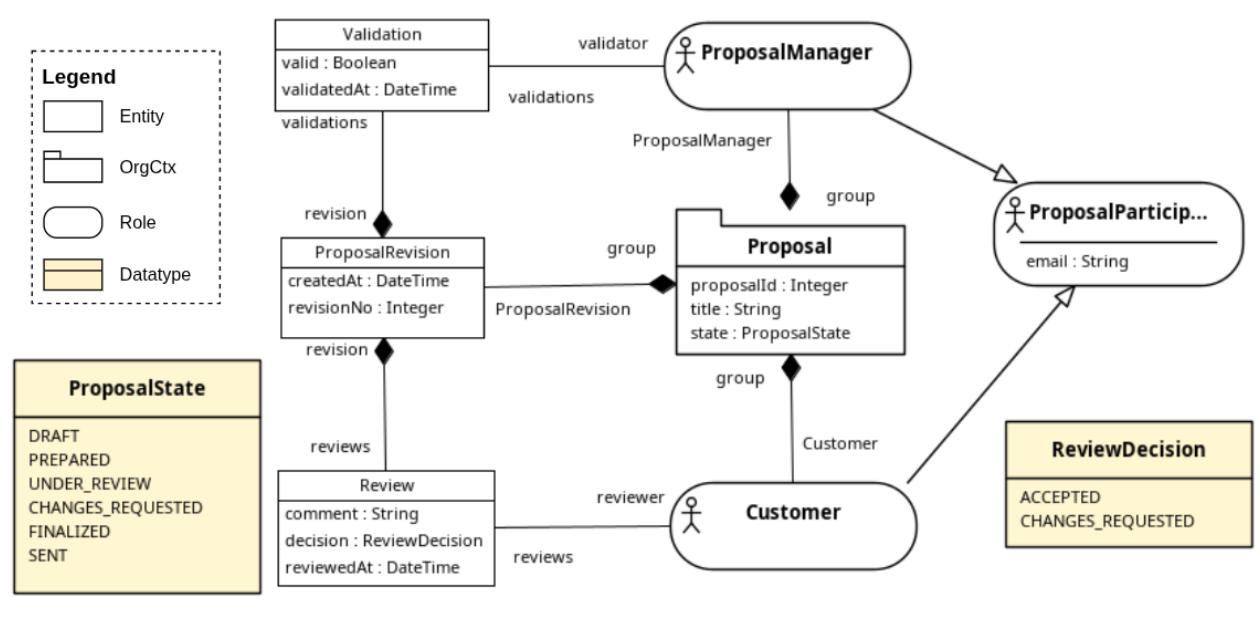
\includegraphics[width=3.189in,height=\textheight]{figures/fig-1-1.png}
\caption{Phân tích cú pháp của biểu thức a\%b+c.}\label{fig:1-1}
\end{figure}

Trong ví dụ ở \thesisfigure{fig:1-1}~\cite{ref-30}, hai cây cùng nhận chuỗi a\%b+c nhưng nhóm toán hạng theo hai cách. Cây bên trái nhóm a\%b trước khi cộng với c, còn cây bên phải nhóm b+c thành toán hạng của phép \%. Nếu \% có độ ưu tiên cao hơn +, cách nhóm thứ nhất được chọn. Ví dụ cho thấy một chuỗi có thể thuộc ngôn ngữ dù vẫn cần thêm quy tắc để xác định cấu trúc của nó.

Cú pháp trừu tượng giữ lại những thông tin mà việc kiểm tra và diễn giải cần đến. Chẳng hạn, nút phép toán trong cây cú pháp trừu tượng (Abstract Syntax Tree, AST) phải ghi toán tử và các toán hạng, nhưng có thể bỏ dấu ngoặc nếu cấu trúc cây đã thể hiện cách nhóm~\cite{ref-27}. Với DSL mô hình hóa, cú pháp trừu tượng còn có thể là một mô hình gồm các phần tử liên kết với nhau, trong đó một phần tử có thể tham chiếu đến khai báo ở nơi khác~\cite{ref-27}.

Siêu mô hình (metamodel) định nghĩa các loại phần tử có thể xuất hiện trong mô hình, kiểu của thuộc tính, quan hệ kế thừa, các liên kết được phép và bội số của chúng. Một mô hình tuân thủ siêu mô hình khi các phần tử và mối liên hệ của nó thỏa mãn những quy tắc cấu trúc đó~\cite{ref-14}. Trong phát triển hướng mô hình, siêu mô hình là cơ sở để định nghĩa ngôn ngữ mô hình hóa cho miền ứng dụng~\cite{ref-3}. Trong kiến trúc mô hình nhiều tầng, M0 chứa các thể hiện được mô tả, M1 chứa mô hình cụ thể, M2 chứa siêu mô hình quy định cấu trúc của mô hình M1, còn M3 cung cấp các khái niệm dùng để xây dựng siêu mô hình~\cite{ref-14}.

\begin{figure}
\centering
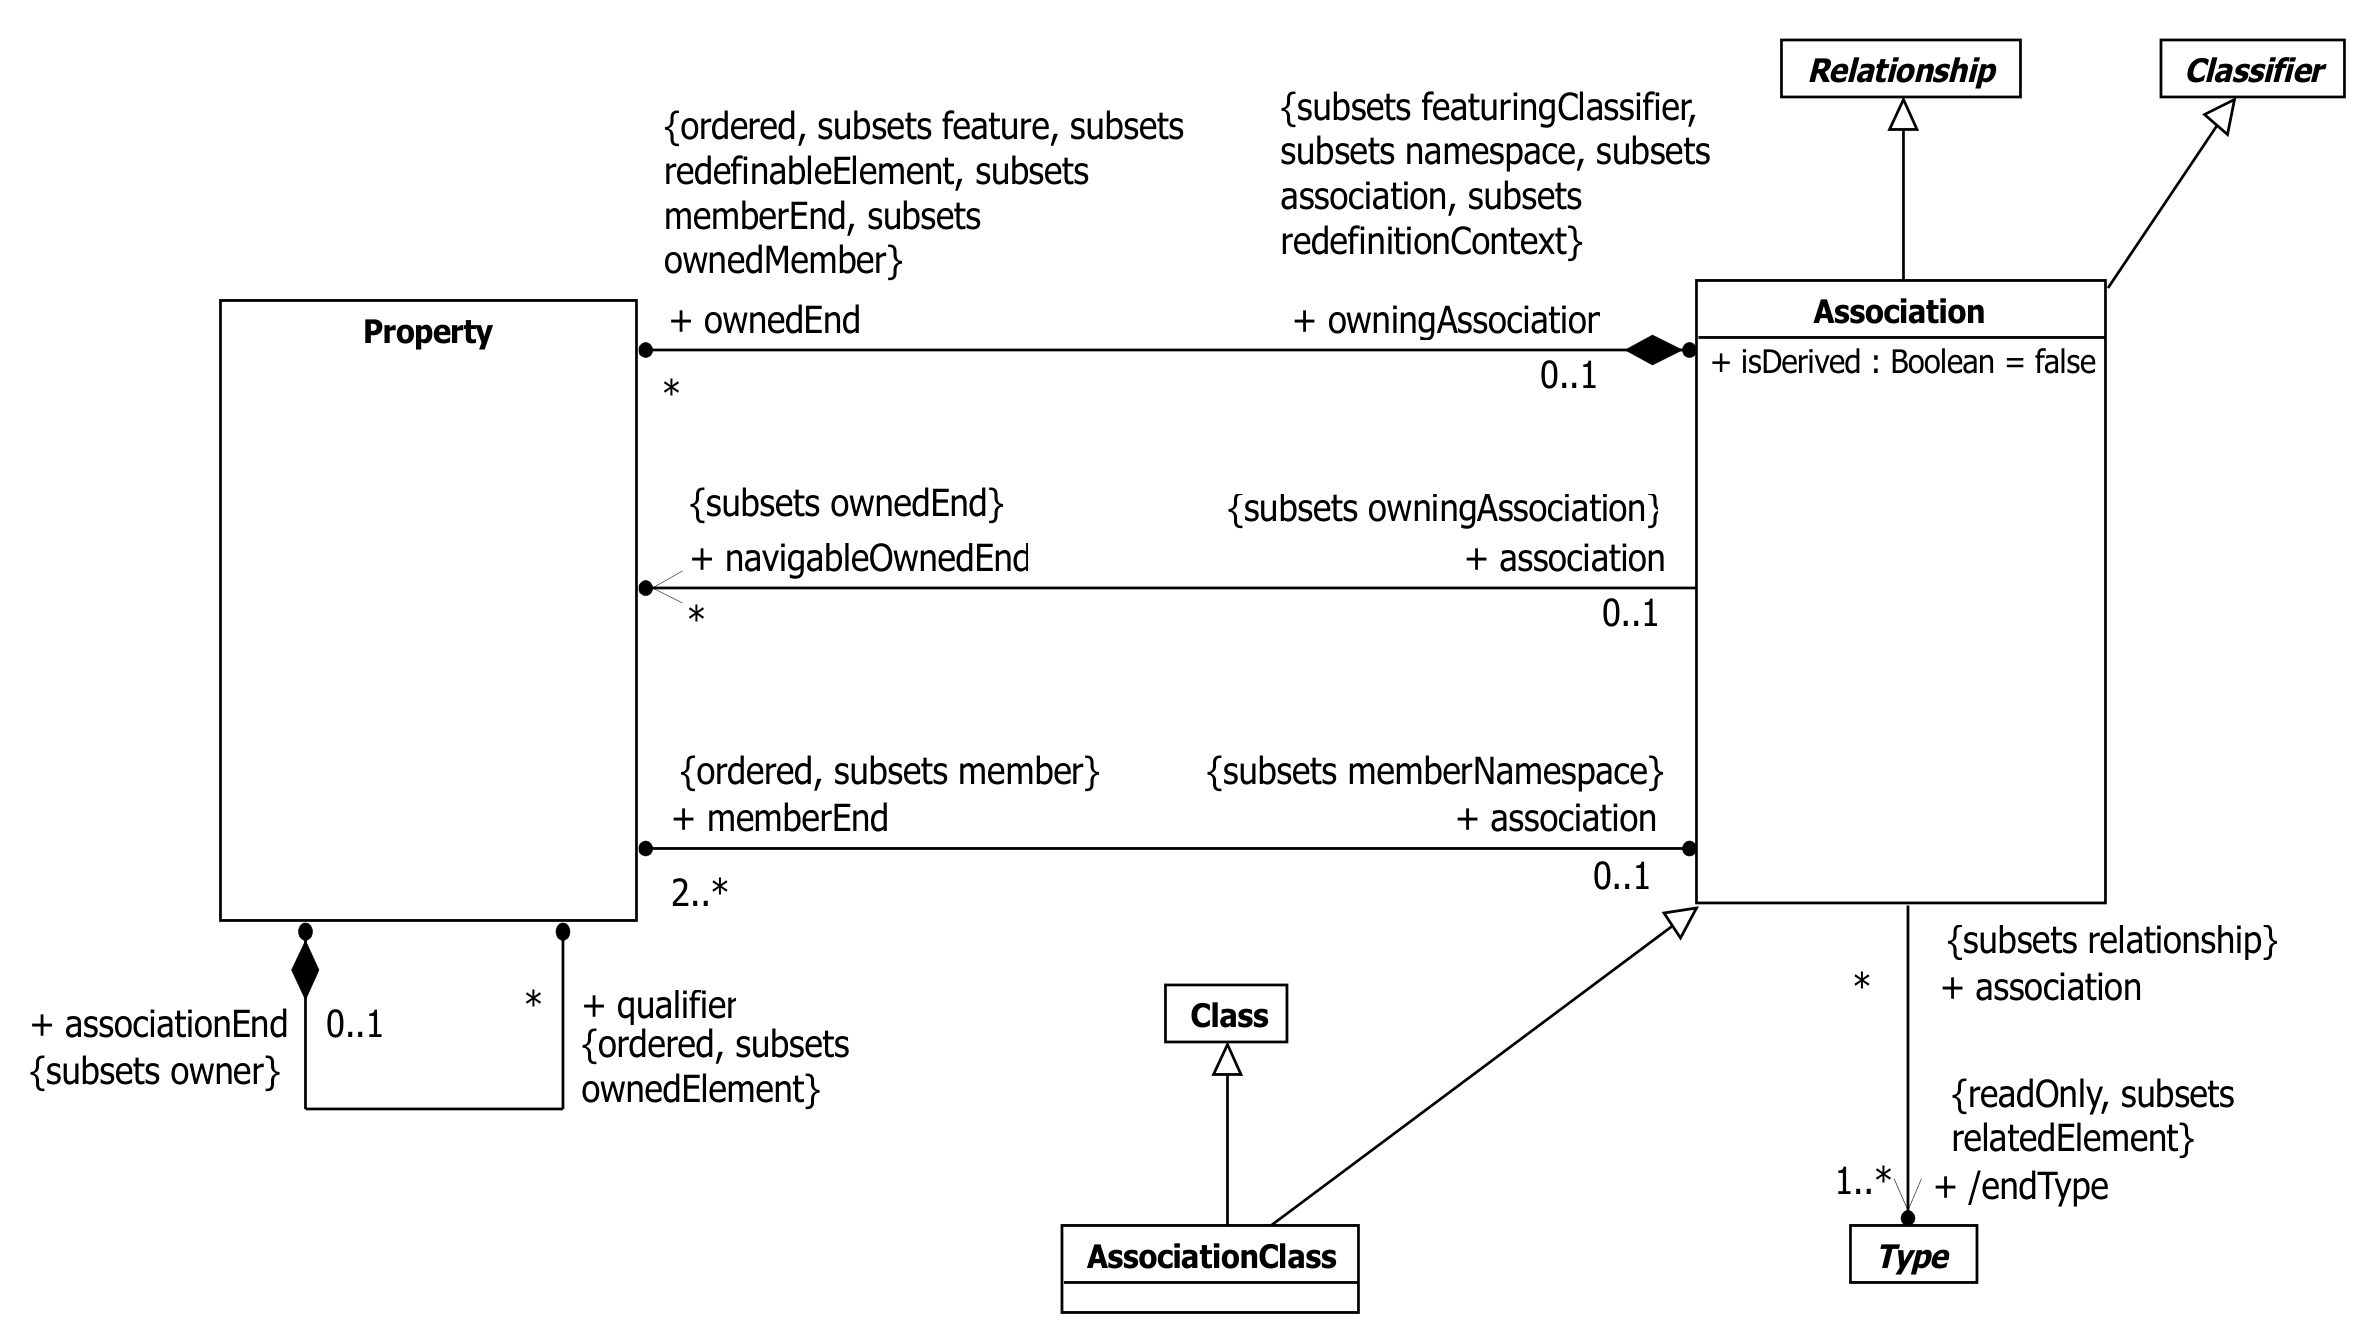
\includegraphics[width=5.9843in,height=\textheight]{figures/fig-1-2.png}
\caption{Liên kết trong siêu mô hình UML.}\label{fig:1-2}
\end{figure}

\thesisfigure{fig:1-2} trích một phần siêu mô hình UML về liên kết~\cite{ref-14}. Trong đó, bội số 2..* của memberEnd yêu cầu mỗi Association có ít nhất hai đầu, mỗi đầu là một Property xác định kiểu của đầu tương ứng. Vì AssociationClass kế thừa cả Association và Class, nó có thể biểu diễn một liên kết mang thuộc tính riêng. Đây là các yêu cầu được kiểm tra trên mô hình lớp trước khi xét một trạng thái đối tượng cụ thể~\cite{ref-14}.

Ngữ nghĩa tĩnh quy định những điều kiện có thể kiểm tra ngay trên đặc tả, như sự hợp lệ của tên tham chiếu hoặc kiểu của biểu thức~\cite{ref-15}. Ngữ nghĩa động giải thích các khai báo được hiểu như thế nào trên trạng thái hoặc qua những lần chuyển trạng thái. Với Association trong UML, yêu cầu về số đầu thuộc cấu trúc của mô hình. Khi xét một trạng thái cụ thể, liên kết được biểu diễn bằng một bộ các thể hiện phù hợp với kiểu của từng đầu~\cite{ref-14}. Trên trạng thái đó, OCL cho phép đánh giá thêm những bất biến do người đặc tả khai báo~\cite{ref-15}.

\subsection{ANTLR và quy trình xử lý ngôn ngữ}\label{sec:1-2-3}

ANTLR (ANother Tool for Language Recognition) sinh bộ phân tích từ vựng (lexer) và bộ phân tích cú pháp (parser) từ mô tả ngữ pháp~\cite{ref-7}. Ngữ pháp ANTLR 4 dùng các cấu trúc kiểu EBNF (Extended Backus--Naur Form) để mô tả thứ tự, phương án thay thế và số lần xuất hiện của các thành phần. Dấu \textbar{} phân cách các phương án, ? biểu thị tùy chọn, còn * và + biểu thị lặp lần lượt từ không hoặc từ một lần. Tên quy tắc lexer bắt đầu bằng chữ hoa và tên quy tắc parser bắt đầu bằng chữ thường~\cite{ref-31}.

\begin{figure}
\centering
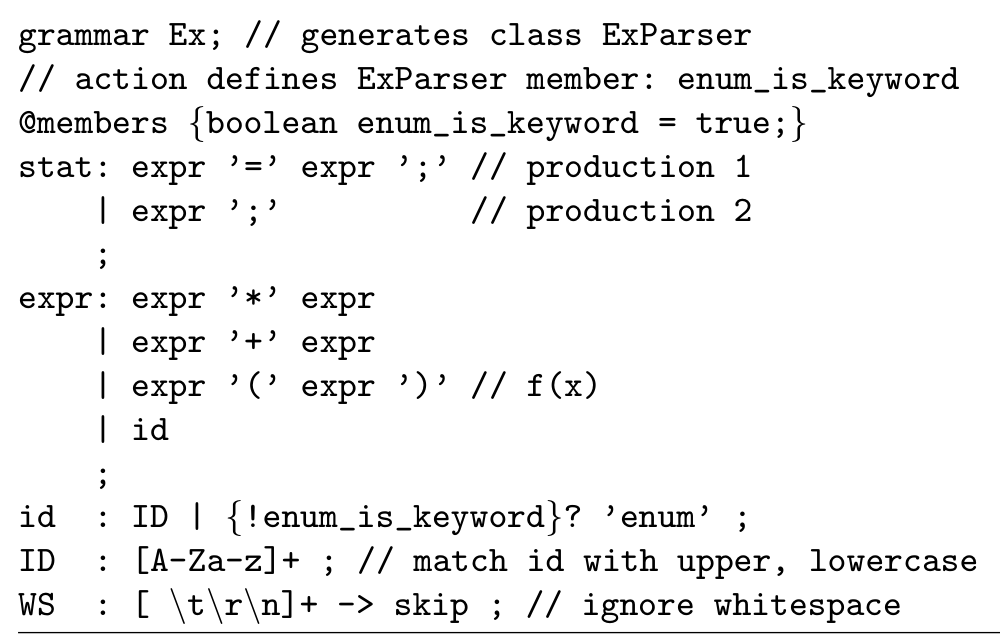
\includegraphics[width=5.1969in,height=\textheight]{figures/fig-1-3.png}
\caption{Ngữ pháp Ex trong ANTLR.}\label{fig:1-3}
\end{figure}

Ngữ pháp Ex trong \thesisfigure{fig:1-3}~\cite{ref-30} cho thấy cách hai nhóm quy tắc phối hợp. Ở bước phân tích từ vựng, ID nhận diện định danh gồm một hoặc nhiều chữ cái, còn WS nhận diện dãy ký tự trắng để bỏ qua bằng lệnh skip. Sau khi nhận token, parser dùng stat, expr và id để nhận diện câu lệnh, biểu thức và vị trí của định danh. Hai phương án của stat cùng bắt đầu bằng expr và kết thúc bằng dấu chấm phẩy, nên parser cần xem các token tiếp theo để nhận ra đó là phép gán hay một biểu thức đứng độc lập~\cite{ref-30}.

Lexer chuyển luồng ký tự thành dãy token có loại, nội dung và vị trí, nhờ đó công cụ có thể chỉ ra nơi phát sinh lỗi~\cite{ref-31}. Với a=b+c; trong ngữ pháp Ex, lexer xếp a, b và c vào loại ID. Parser bắt đầu ở stat, nhận diện phương án gán rồi áp dụng expr cho hai vế~\cite{ref-30}. Cây phân tích ghi lại quy tắc được áp dụng và các token được nhận diện. Vì parser có thể phục hồi sau một số lỗi để tiếp tục chẩn đoán, cần đọc thông báo lỗi cùng với cây trước khi kết luận đầu vào hợp lệ~\cite{ref-31}.

ANTLR 4 dùng Adaptive LL(*) để chọn phương án dựa trên các token phía trước và ngữ cảnh khi cần. Trong ngữ pháp Ex, một số phương án của expr bắt đầu bằng chính expr, tạo thành đệ quy trái trực tiếp. ANTLR 4 có thể chuyển đổi các dạng đệ quy trái trực tiếp được hỗ trợ, nhờ đó ngữ pháp vẫn gần với cách mô tả biểu thức trong khi parser xử lý được độ ưu tiên và tính kết hợp~\cite{ref-30}.

Chương trình có thể xử lý cây phân tích bằng listener hoặc visitor. Listener nhận sự kiện khi bộ duyệt đi vào và đi ra khỏi mỗi nút quy tắc, còn visitor chủ động chọn các nút con cần thăm và có thể trả kết quả cho nút cha~\cite{ref-31}. Khi cần tạo AST hoặc một mô hình tuân theo siêu mô hình, lớp xử lý cây quyết định mỗi cấu trúc cú pháp sẽ trở thành phần tử nào trong mô hình đích.

Ở bước phân tích ngữ nghĩa, bảng ký hiệu có thể lưu tên, kiểu và phạm vi của các khai báo. Từ đó có thể giải quyết tham chiếu, phát hiện khai báo trùng hoặc kiểm tra kiểu toán hạng~\cite{ref-27}. Chẳng hạn, parser có thể nhận diện vế phải b+c theo quy tắc expr của Ex~\cite{ref-30}. Trong một DSL sử dụng ngữ pháp tương tự, việc phép cộng đó có hợp lệ hay không còn phụ thuộc b và c có được khai báo với kiểu phù hợp theo quy tắc của ngôn ngữ. Phân tách các bước này giúp nhận diện lỗi từ vựng, lỗi cú pháp và lỗi ngữ nghĩa tại đúng mức mô tả~\cite{ref-27}.

\section{Hệ thống đa tác tử và JaCaMo}\label{sec:1-3}

Hệ thống đa tác tử (Multi-Agent System, MAS) gồm nhiều tác tử có khả năng hành động và tương tác. Tính tự chủ, khả năng tương tác xã hội, tính phản ứng và khả năng chủ động theo đuổi mục tiêu là những đặc trưng thường dùng để mô tả tác tử~\cite{ref-1}. Trong một MAS, kết quả của hành động còn phụ thuộc vào môi trường mà tác tử tác động tới và cách tổ chức hoạt động của các tác tử~\cite{ref-2}.

\subsection{Tổng quan hệ thống đa tác tử và kiến trúc JaCaMo}\label{sec:1-3-1}

Hệ thống đa tác tử có nguồn gốc từ hướng trí tuệ nhân tạo phân tán (Distributed Artificial Intelligence, DAI) vào cuối thập niên 1970 và đầu thập niên 1980. Các công trình ban đầu xem xét cách nhiều thành phần tính toán phối hợp giải một bài toán khi mỗi thành phần chỉ có một phần thông tin hoặc năng lực xử lý~\cite{ref-32}. Một mốc tiêu biểu là giao thức Contract Net do Reid G. Smith công bố năm 1980. Giao thức này phân công việc bằng cách công bố nhiệm vụ, nhận đề xuất từ các nút có khả năng thực hiện rồi giao nhiệm vụ cho nút phù hợp~\cite{ref-33}. Đến năm 1988, Alan H. Bond và Les Gasser tập hợp các công trình của hướng nghiên cứu trên trong cuốn Readings in Distributed Artificial Intelligence~\cite{ref-32}.

Từ bài toán phân chia công việc chung, nghiên cứu mở rộng sang việc thiết kế các tác tử có thông tin, mục tiêu và khả năng ra quyết định riêng. Trong thập niên 1990, Wooldridge và Jennings hệ thống hóa các đặc trưng và kiến trúc tác tử~\cite{ref-1}, còn tuyển tập Multiagent Systems do Gerhard Weiss biên tập nối phân tích hành động cá nhân với bài toán phối hợp tập thể~\cite{ref-34}. Đến năm 2002, Foundation for Intelligent Physical Agents (FIPA) chuẩn hóa các thông điệp của Contract Net, từ mời và tiếp nhận đề xuất đến chấp nhận, từ chối và thông báo kết quả~\cite{ref-35}.

Lập trình hệ đa tác tử cần mô tả cách tác tử chọn hành động, môi trường mà hành động tác động tới và những quy tắc phối hợp trong tổ chức. Boissier và cộng sự tích hợp ba chiều đó trong JaCaMo, được trình bày trong công trình công bố năm 2013~\cite{ref-2}. Sách Multi-Agent Oriented Programming sau đó trình bày cách vận dụng nền tảng qua các bài tập và ví dụ lập trình~\cite{ref-36}.

Ba chiều của JaCaMo cung cấp thông tin khác nhau về cùng một hoạt động. Jason hỗ trợ tác tử suy luận bằng belief, goal, plan và intention. Một hành động được chọn trong plan có thể gọi thao tác của artifact trong CArtAgO hoặc góp phần thực hiện nhiệm vụ đã cam kết trong tổ chức Moise~\cite{ref-2}. Workspace xác định phạm vi sử dụng và quan sát artifact, còn nhóm, vai trò và mission mô tả cách phối hợp để đạt mục tiêu chung. Sự phân chia này giúp nhận diện một hoạt động đã thay đổi thông tin mà tác tử sử dụng, dữ liệu môi trường hay quan hệ đảm nhiệm vai trò~\cite{ref-2}.

\subsection{Belief, Goal, Plan và Intention trong Jason}\label{sec:1-3-2}

Jason là trình thông dịch cho một phiên bản mở rộng của AgentSpeak~\cite{ref-8}. Trong cách lập trình dựa trên kiến trúc Belief--Desire--Intention (BDI), tác tử suy luận từ cơ sở niềm tin (belief base) và có thể phân biệt niềm tin do cảm nhận với niềm tin do tác tử khác cung cấp~\cite{ref-9}. Mục tiêu đạt được (achievement goal), ký hiệu bằng !, khiến tác tử tìm một kế hoạch để thực hiện. Mục tiêu truy vấn (test goal), ký hiệu bằng ?, tìm dữ liệu trong cơ sở niềm tin có thể hợp nhất với biểu thức cần kiểm tra~\cite{ref-37}.

Một kế hoạch (plan) có dạng te : ct \textless- h, trong đó te là sự kiện kích hoạt, ct là ngữ cảnh áp dụng và h là thân kế hoạch. Một kế hoạch liên quan khi te hợp nhất được với sự kiện đã chọn và có thể áp dụng khi cơ sở niềm tin hiện tại thỏa ct~\cite{ref-37}. Thân kế hoạch quy định chuỗi hành động, mục tiêu con hoặc thao tác cập nhật niềm tin. Việc thêm hoặc xóa niềm tin có thể tạo sự kiện mới, lần lượt biểu thị bằng dấu + hoặc − ở sự kiện kích hoạt~\cite{ref-37}.

Ý định (intention) biểu diễn hướng hành động mà tác tử đã chọn và có thể xem như một ngăn xếp các kế hoạch đang thực hiện. Khi thân kế hoạch phát sinh mục tiêu con, sự kiện nội bộ vẫn gắn với ý định hiện tại và kế hoạch được chọn cho mục tiêu con được đưa lên đỉnh ngăn xếp~\cite{ref-37}. Khi kế hoạch con kết thúc, tác tử trở lại kế hoạch bên dưới. Một sự kiện bên ngoài, chẳng hạn sự kiện do thay đổi niềm tin, có thể tạo một ý định mới~\cite{ref-37}.

\begin{figure}
\centering
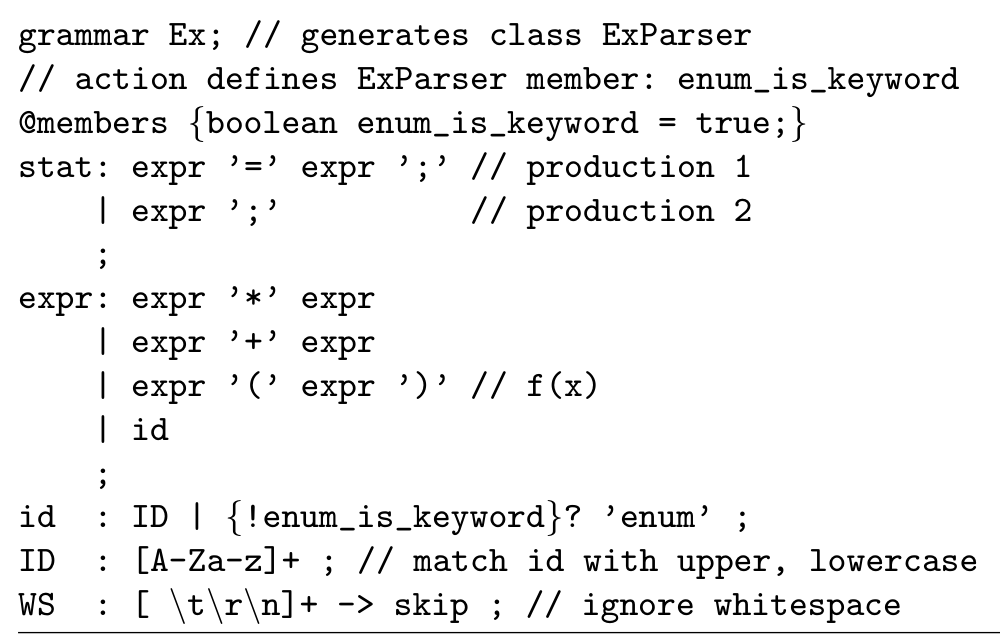
\includegraphics[width=6.2in,height=\textheight]{figures/fig-1-4.png}
\caption{Chu trình diễn giải AgentSpeak(L).}\label{fig:1-4}
\end{figure}

\thesisfigure{fig:1-4} dùng sơ đồ của Machado và Bordini (2002) để mô tả chu trình diễn giải của AgentSpeak(L)~\cite{ref-37}. Cảm nhận từ môi trường có thể cập nhật niềm tin và sinh sự kiện. Bộ thông dịch chọn sự kiện (\(S_{e}\)), tìm các kế hoạch có sự kiện kích hoạt phù hợp và xét ngữ cảnh để chọn kế hoạch áp dụng được (\(S_{o}\)). Kế hoạch này tạo hoặc cập nhật ý định. Sau đó, bộ thông dịch chọn ý định (\(S_{i}\)) để thực hiện bước kế tiếp, chẳng hạn tác động lên môi trường, truy vấn niềm tin hoặc tạo mục tiêu con~\cite{ref-37}.

\begin{figure}
\centering
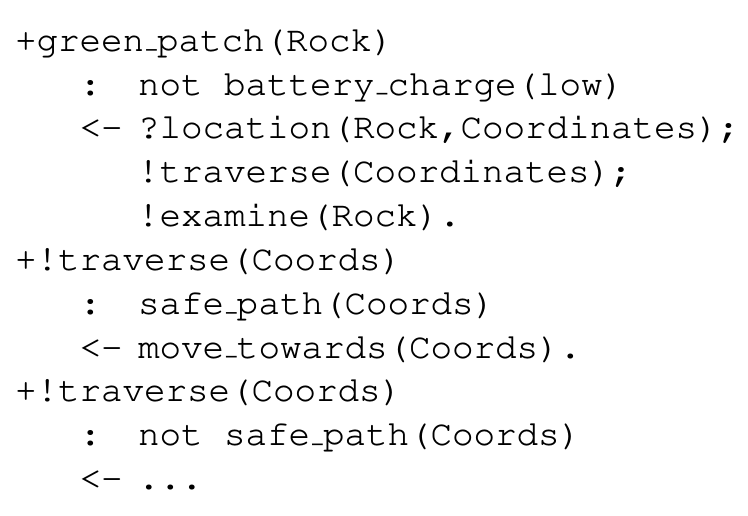
\includegraphics[width=4.1732in,height=\textheight]{figures/fig-1-5.png}
\caption{Kế hoạch AgentSpeak cho robot thăm dò Sao Hỏa.}\label{fig:1-5}
\end{figure}

Các kế hoạch cho robot thăm dò Sao Hỏa ở \thesisfigure{fig:1-5} là một ví dụ về AgentSpeak~\cite{ref-29}. Kế hoạch đầu tiên được xét khi niềm tin green\_patch(Rock) xuất hiện và được áp dụng nếu tác tử chưa tin rằng pin đang yếu. Kế hoạch truy vấn tọa độ mẫu đá bằng ?location rồi đặt mục tiêu di chuyển tới mẫu và kiểm tra nó. Với sự kiện +!traverse, hai kế hoạch kiểm tra hai điều kiện khác nhau về độ an toàn của đường đi, vì vậy cùng một mục tiêu có thể dẫn đến những hành động khác nhau tùy vào thông tin hiện có~\cite{ref-29}.

\subsection{Artifact và Workspace trong CArtAgO}\label{sec:1-3-3}

Trong JaCaMo, CArtAgO cung cấp mô hình lập trình cho chiều môi trường~\cite{ref-2}. Tác tử có thể dùng artifact để đọc thông tin, thao tác trên tài nguyên hoặc phối hợp với tác tử khác. Khi nhiều tác tử dùng chung một artifact, chúng tương tác qua trạng thái và các quy tắc của artifact. Cách tổ chức này phân biệt quyết định chọn hành động của tác tử với cách môi trường thực hiện hành động ấy~\cite{ref-10}.

CArtAgO tổ chức môi trường thành các workspace, mỗi workspace tập hợp những artifact và tác tử tham gia, kể cả khi môi trường được phân bố qua nhiều nút. Một tác tử có thể tham gia nhiều workspace và tìm, tạo hoặc loại bỏ artifact qua những thao tác mà workspace cung cấp~\cite{ref-38}. Các artifact mà tác tử có thể sử dụng quyết định những hành động môi trường khả dụng tại thời điểm đó. Kiểu artifact quy định cấu trúc và thao tác chung, còn định danh chỉ ra thể hiện cụ thể mà tác tử muốn sử dụng hoặc quan sát~\cite{ref-38}.

Giao diện của artifact cung cấp các thao tác (operation) mà tác tử có thể yêu cầu, trong đó một số thao tác làm thay đổi trạng thái của artifact~\cite{ref-10}. Tác tử đọc những phần đã được công bố của trạng thái qua thuộc tính quan sát được (observable property). Artifact còn có thể phát tín hiệu (signal) để thông báo một sự kiện. Vì vậy, thuộc tính cho biết giá trị hiện hành, còn tín hiệu cho biết điều gì vừa xảy ra~\cite{ref-38}.

\begin{figure}
\centering
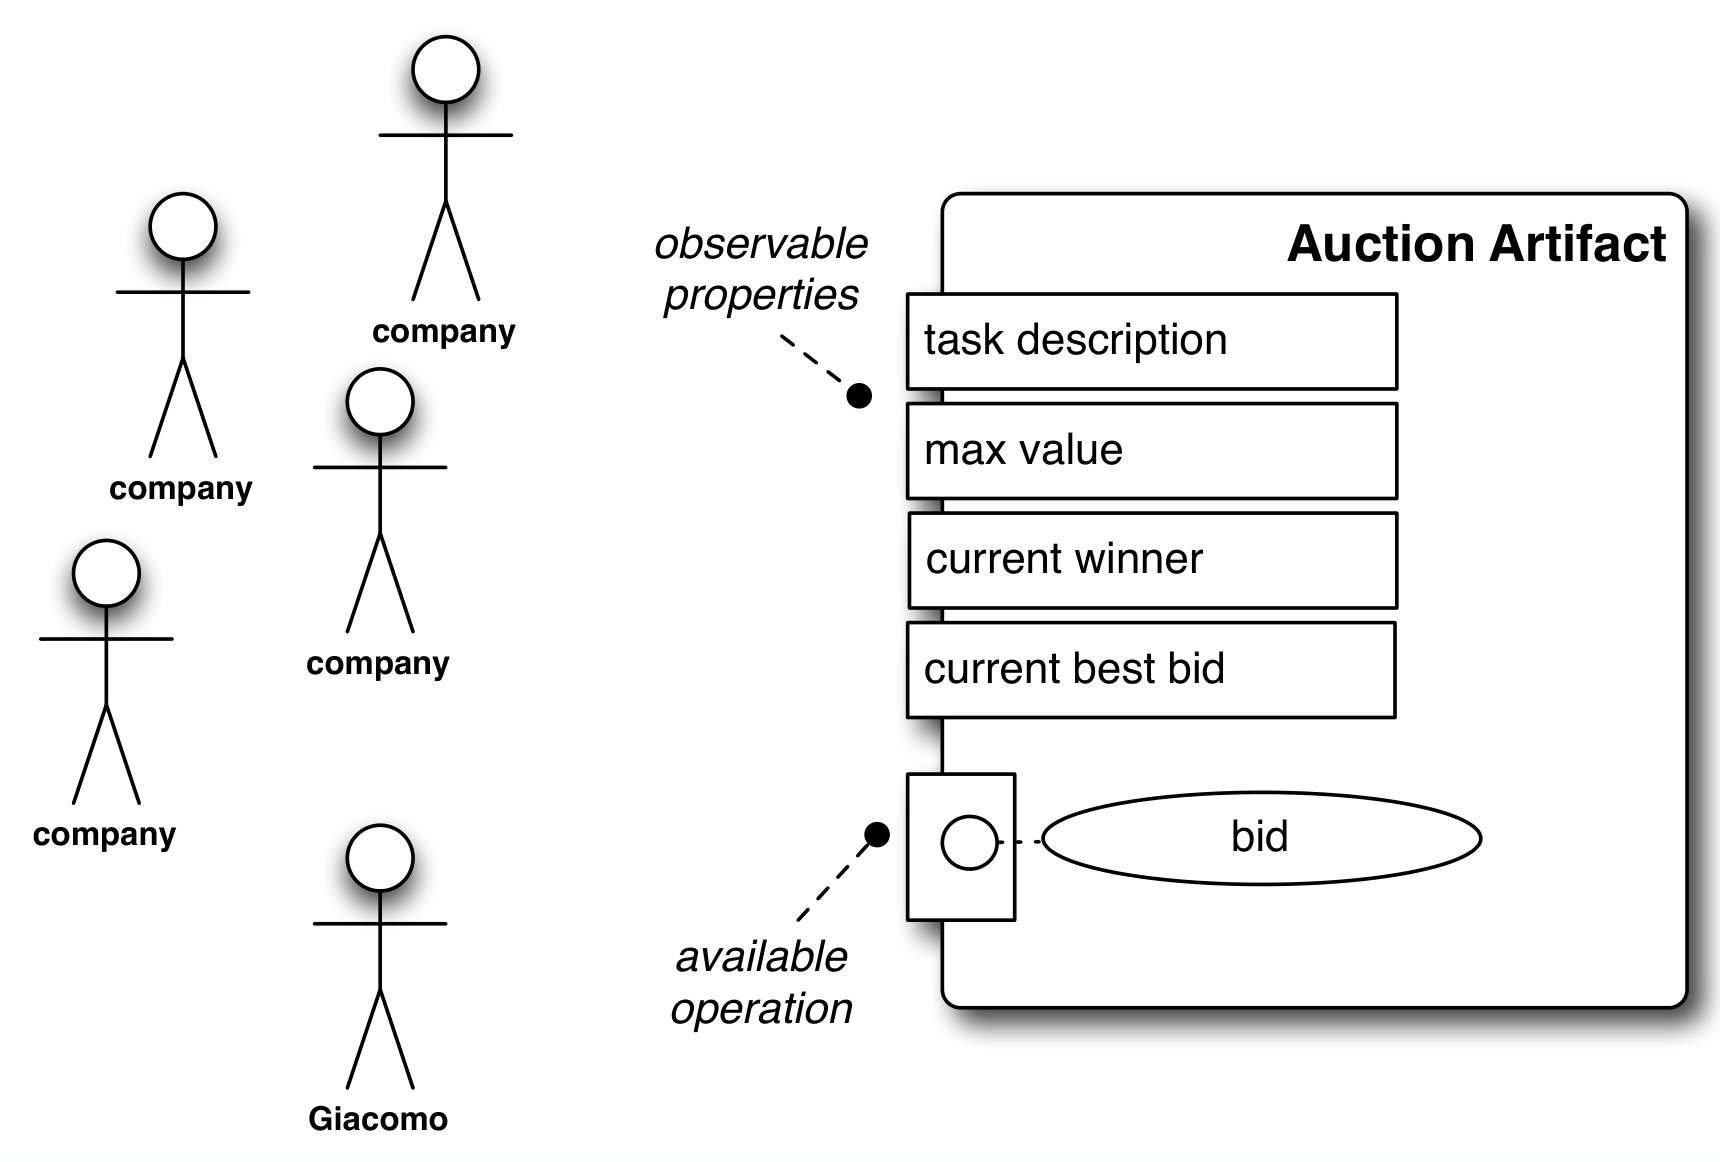
\includegraphics[width=5.5906in,height=\textheight]{figures/fig-1-6.png}
\caption{Giao diện artifact đấu giá.}\label{fig:1-6}
\end{figure}

Artifact trong \thesisfigure{fig:1-6} thuộc ca xây nhà, trong đó chủ nhà Giacomo tạo một cuộc đấu giá cho từng công việc xây dựng~\cite{ref-39}. Mỗi công ty có thể đọc mô tả công việc, mức giá tối đa, bên đang dẫn đầu và giá tốt nhất, rồi gọi thao tác bid để gửi giá. Nhiều công ty có thể theo dõi cùng một cuộc đấu giá. Các cuộc đấu giá dùng chung giao diện nhưng mỗi thể hiện giữ dữ liệu riêng của nó~\cite{ref-39}.

Một tác tử bắt đầu theo dõi artifact bằng focus với định danh của artifact đó. Khi kết hợp với Jason, các thuộc tính quan sát được trở thành belief của tác tử và được cập nhật khi giá trị thay đổi~\cite{ref-38}. Tín hiệu cũng có thể làm phát sinh sự kiện để tác tử chọn kế hoạch phù hợp. Tín hiệu không tự động được lưu thành belief~\cite{ref-38}.

\begin{figure}
\centering
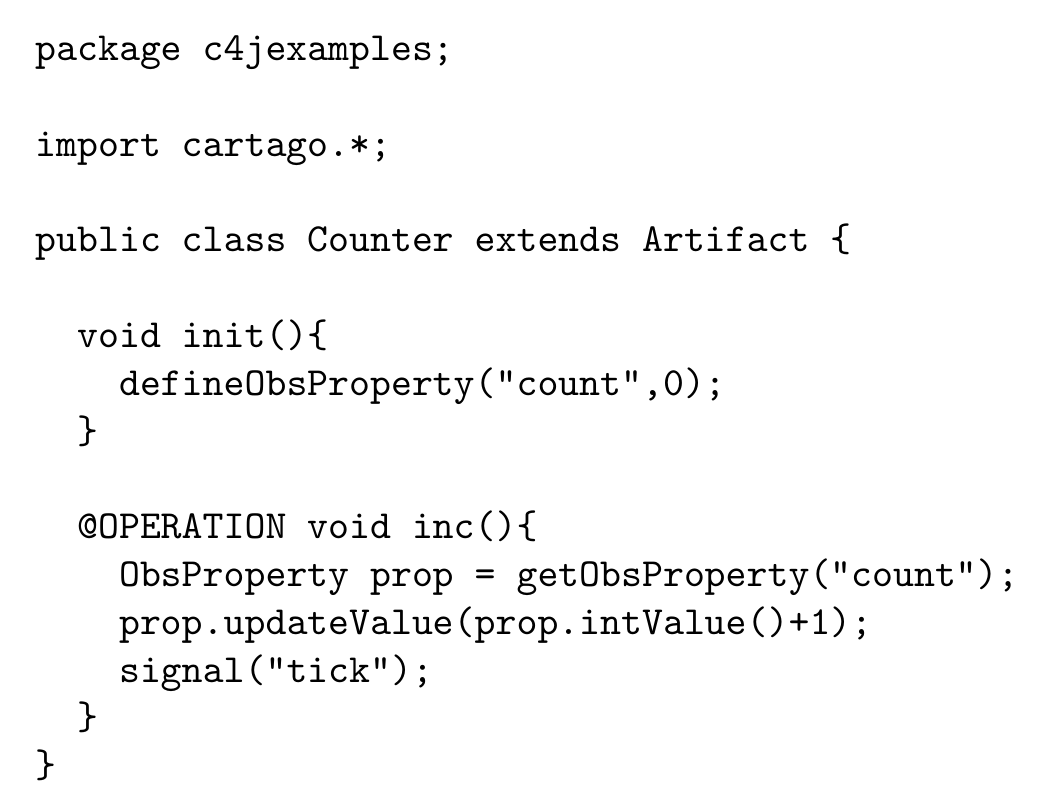
\includegraphics[width=4.6457in,height=\textheight]{figures/fig-1-7.png}
\caption{Định nghĩa artifact Counter.}\label{fig:1-7}
\end{figure}

Ví dụ Counter ở \thesisfigure{fig:1-7} cho thấy sự khác biệt giữa giá trị và sự kiện quan sát từ artifact~\cite{ref-38}. Khi khởi tạo, Counter công bố thuộc tính count với giá trị 0. Mỗi lần thực hiện inc, bộ đếm tăng và artifact phát tín hiệu tick. Tác tử đang theo dõi có thể đọc count để biết giá trị hiện hành hoặc phản ứng với tick khi có một lần tăng.

\subsection{Mô hình tổ chức Moise}\label{sec:1-3-4}

Moise+ mô hình hóa cách một tập tác tử phối hợp để đạt mục tiêu chung~\cite{ref-11}. Đặc tả tổ chức (Organisational Specification, OS) gồm đặc tả cấu trúc (Structural Specification, SS), đặc tả chức năng (Functional Specification, FS) và đặc tả nghĩa vụ (Deontic Specification, DS). Ba phần lần lượt xác định vị trí và quan hệ trong tổ chức, cách phân rã mục tiêu chung, và quyền hoặc nghĩa vụ cam kết thực hiện từng phần công việc~\cite{ref-40}.

Đặc tả cấu trúc của Moise+ xác định vai trò và cách tập hợp các vai trò thành nhóm. Quan hệ chuyên biệt hóa cho phép một vai trò kế thừa đặc điểm của vai trò tổng quát, còn các quan hệ xã hội mô tả khả năng biết đến, giao tiếp hoặc thực thi quyền hạn đối với tác tử ở vai trò khác~\cite{ref-40}. Mỗi nhóm quy định các vai trò có thể cùng được đảm nhiệm và giới hạn số tác tử của từng vai trò. Ví dụ, nhóm phòng ngự yêu cầu một thủ môn và ba hậu vệ. Quyền hạn của thủ môn đối với hậu vệ chỉ áp dụng trong nhóm phòng ngự, còn quyền hạn của huấn luyện viên có thể vươn tới những nhóm khác~\cite{ref-40}.

Đặc tả chức năng tổ chức mục tiêu chung thành các lược đồ phối hợp (social scheme). Mỗi lược đồ có mục tiêu gốc và các kế hoạch phân rã mục tiêu. Phép phân rã tuần tự yêu cầu đạt các mục tiêu con theo thứ tự, phép lựa chọn yêu cầu đạt một trong các mục tiêu thay thế và phép song song yêu cầu đạt tất cả nhưng cho phép thực hiện đồng thời~\cite{ref-40}. Một mission gom những mục tiêu có liên quan thành phần việc mà tác tử có thể cam kết thực hiện~\cite{ref-40}.

\begin{figure}
\centering
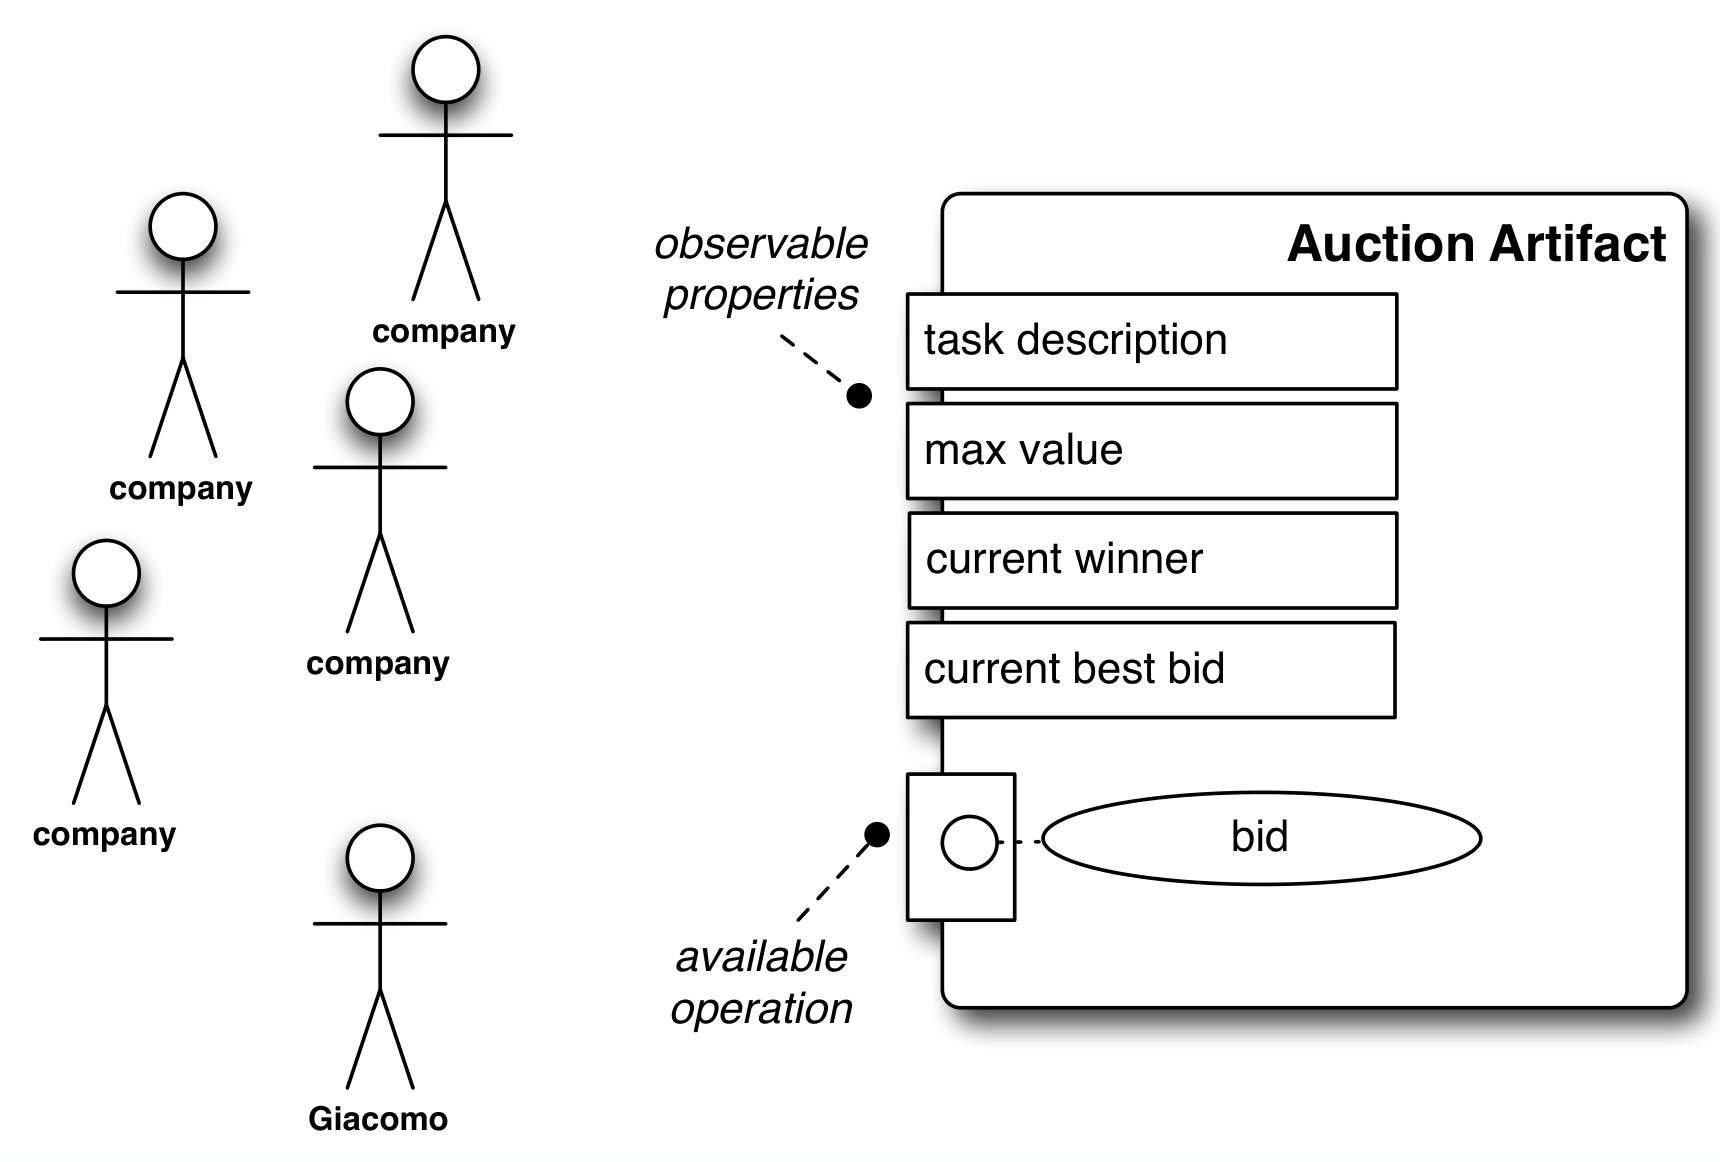
\includegraphics[width=5.9843in,height=\textheight]{figures/fig-1-8.png}
\caption{Lược đồ mục tiêu của phương án tấn công biên.}\label{fig:1-8}
\end{figure}

Trong lược đồ ở \thesisfigure{fig:1-8}~\cite{ref-40}, mục tiêu ghi bàn được phân rã thành những bước như giành bóng, đưa bóng tới khu vực tấn công và dứt điểm. Mission m3 gắn việc có mặt trong khu vực cầu môn đối phương và dứt điểm với mục tiêu chung là ghi bàn.

Đặc tả nghĩa vụ kết nối vai trò với mission. Một quyền (permission) cho phép tác tử giữ vai trò tương ứng cam kết với mission, còn nghĩa vụ (obligation) yêu cầu cam kết khi luật áp dụng~\cite{ref-40}. Trong lược đồ tấn công biên, hậu vệ được phép cam kết với m1, còn tiền vệ và tiền đạo lần lượt có nghĩa vụ với m2 và m3. Thứ tự thực hiện vẫn do lược đồ quy định, chẳng hạn tiền vệ theo đuổi mục tiêu có mặt ở giữa sân sau khi mục tiêu giành bóng đã đạt~\cite{ref-40}.

Thực thể tổ chức (Organisational Entity, OE) là một thể hiện của đặc tả. OE ghi nhận các nhóm đã tạo, tác tử đang đảm nhiệm từng vai trò và các cam kết đã hình thành~\cite{ref-40}. Vì các quan hệ này thay đổi khi hệ chạy, một nhóm đã được tạo vẫn có thể chưa đáp ứng đủ bội số.

\begin{figure}
\centering
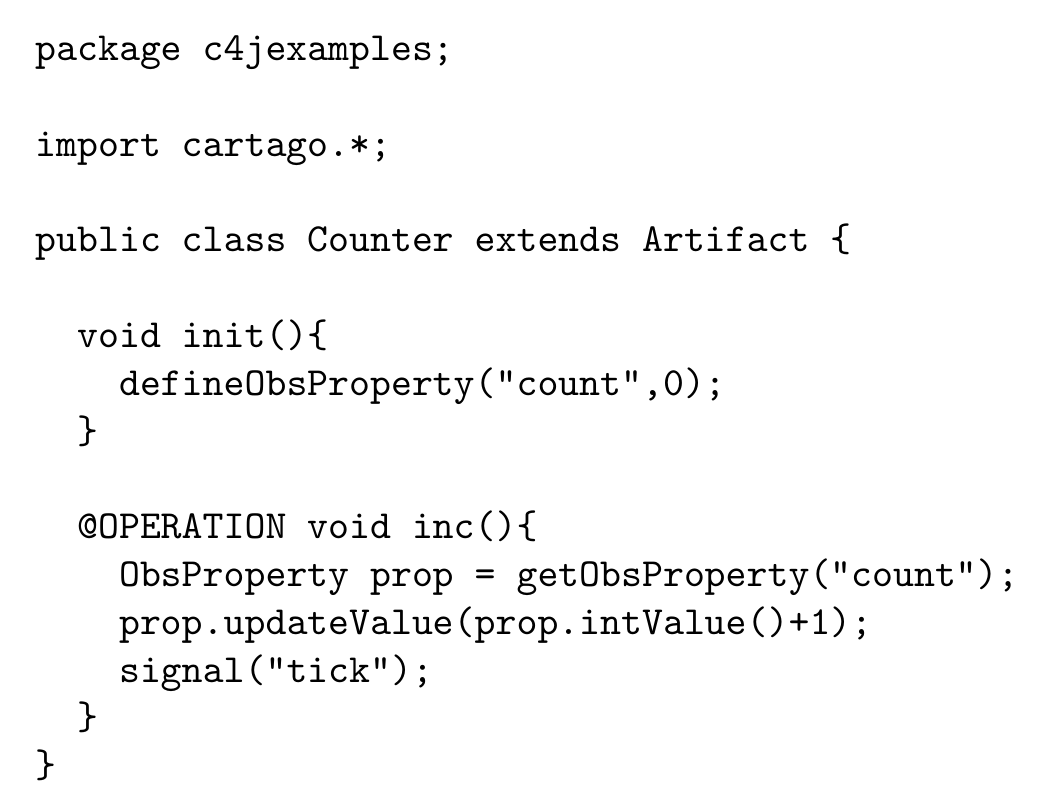
\includegraphics[width=4.4252in,height=\textheight]{figures/fig-1-9.png}
\caption{Thể hiện nhóm phòng ngự trong S-Moise+.}\label{fig:1-9}
\end{figure}

Thể hiện nhóm phòng ngự ở \thesisfigure{fig:1-9}~\cite{ref-40} có tác tử Marcos đảm nhiệm vai trò thủ môn, nhưng chưa có hậu vệ nào so với mức tối thiểu là ba. Ví dụ này cho thấy cách dùng đặc tả làm tiêu chí và dùng dữ liệu của thực thể tổ chức để đánh giá nhóm tại một thời điểm.

\section{Mô hình mục tiêu iStar}\label{sec:1-4}

iStar 2.0 là ngôn ngữ mô hình hóa hướng mục tiêu cho các hệ thống có nhiều chủ thể. Hướng dẫn của Dalpiaz, Franch và Horkoff mô tả cách biểu diễn ý định của mỗi chủ thể, những cách thực hiện ý định và quan hệ phụ thuộc giữa các bên~\cite{ref-12}. Các ví dụ của công cụ piStar minh họa cách thể hiện những khái niệm đó trên biểu đồ~\cite{ref-41}.

\subsection{Actor và các phần tử ý định}\label{sec:1-4-1}

Actor biểu diễn chủ thể có ý định và có thể hành động để đạt ý định đó. Khi cần phân loại chi tiết hơn, mô hình dùng Agent để chỉ cá nhân hoặc hệ thống cụ thể, và dùng Role để chỉ trách nhiệm hoặc hành vi trong một ngữ cảnh~\cite{ref-12}. Ký pháp của Actor là hình tròn, Agent có thêm nét ngang ở phía trên và Role có thêm nét cong ở đáy. Đường bao nét đứt phân định phạm vi ý định của chủ thể~\cite{ref-12}.

Trong phạm vi của một chủ thể, Goal ghi nhận trạng thái mong muốn có tiêu chí đạt tương đối rõ, còn Task chỉ một cách thực hiện công việc. Hai loại phần tử này lần lượt được vẽ bằng hình chữ nhật bo góc và hình lục giác~\cite{ref-12}. Một tài nguyên vật chất hoặc thông tin được biểu diễn bằng Resource có hình chữ nhật. Khi cần mô tả đặc tính mong muốn của quá trình, kết quả hay tài nguyên, mô hình dùng Quality có hai cạnh uốn lượn~\cite{ref-12}.

Siêu mô hình Ecore của Ayala và cộng sự hiện thực hóa các kiểu được mô tả trong hướng dẫn iStar 2.0~\cite{ref-12}. Trong tệp đó, Agent và Role chuyên biệt hóa Actor, còn tham chiếu wants nối chủ thể với các phần tử ý định. Goal, Task, Resource và Quality cùng chuyên biệt hóa IntentionalElement~\cite{ref-42}. Quan hệ Dependency là một lớp riêng với ba tham chiếu bắt buộc depender, dependee và dependum. Hai tham chiếu dependerElmt và dependeeElmt là tùy chọn, qua đó siêu mô hình giới hạn những cấu trúc phụ thuộc hợp lệ~\cite{ref-42}.

\begin{figure}
\centering
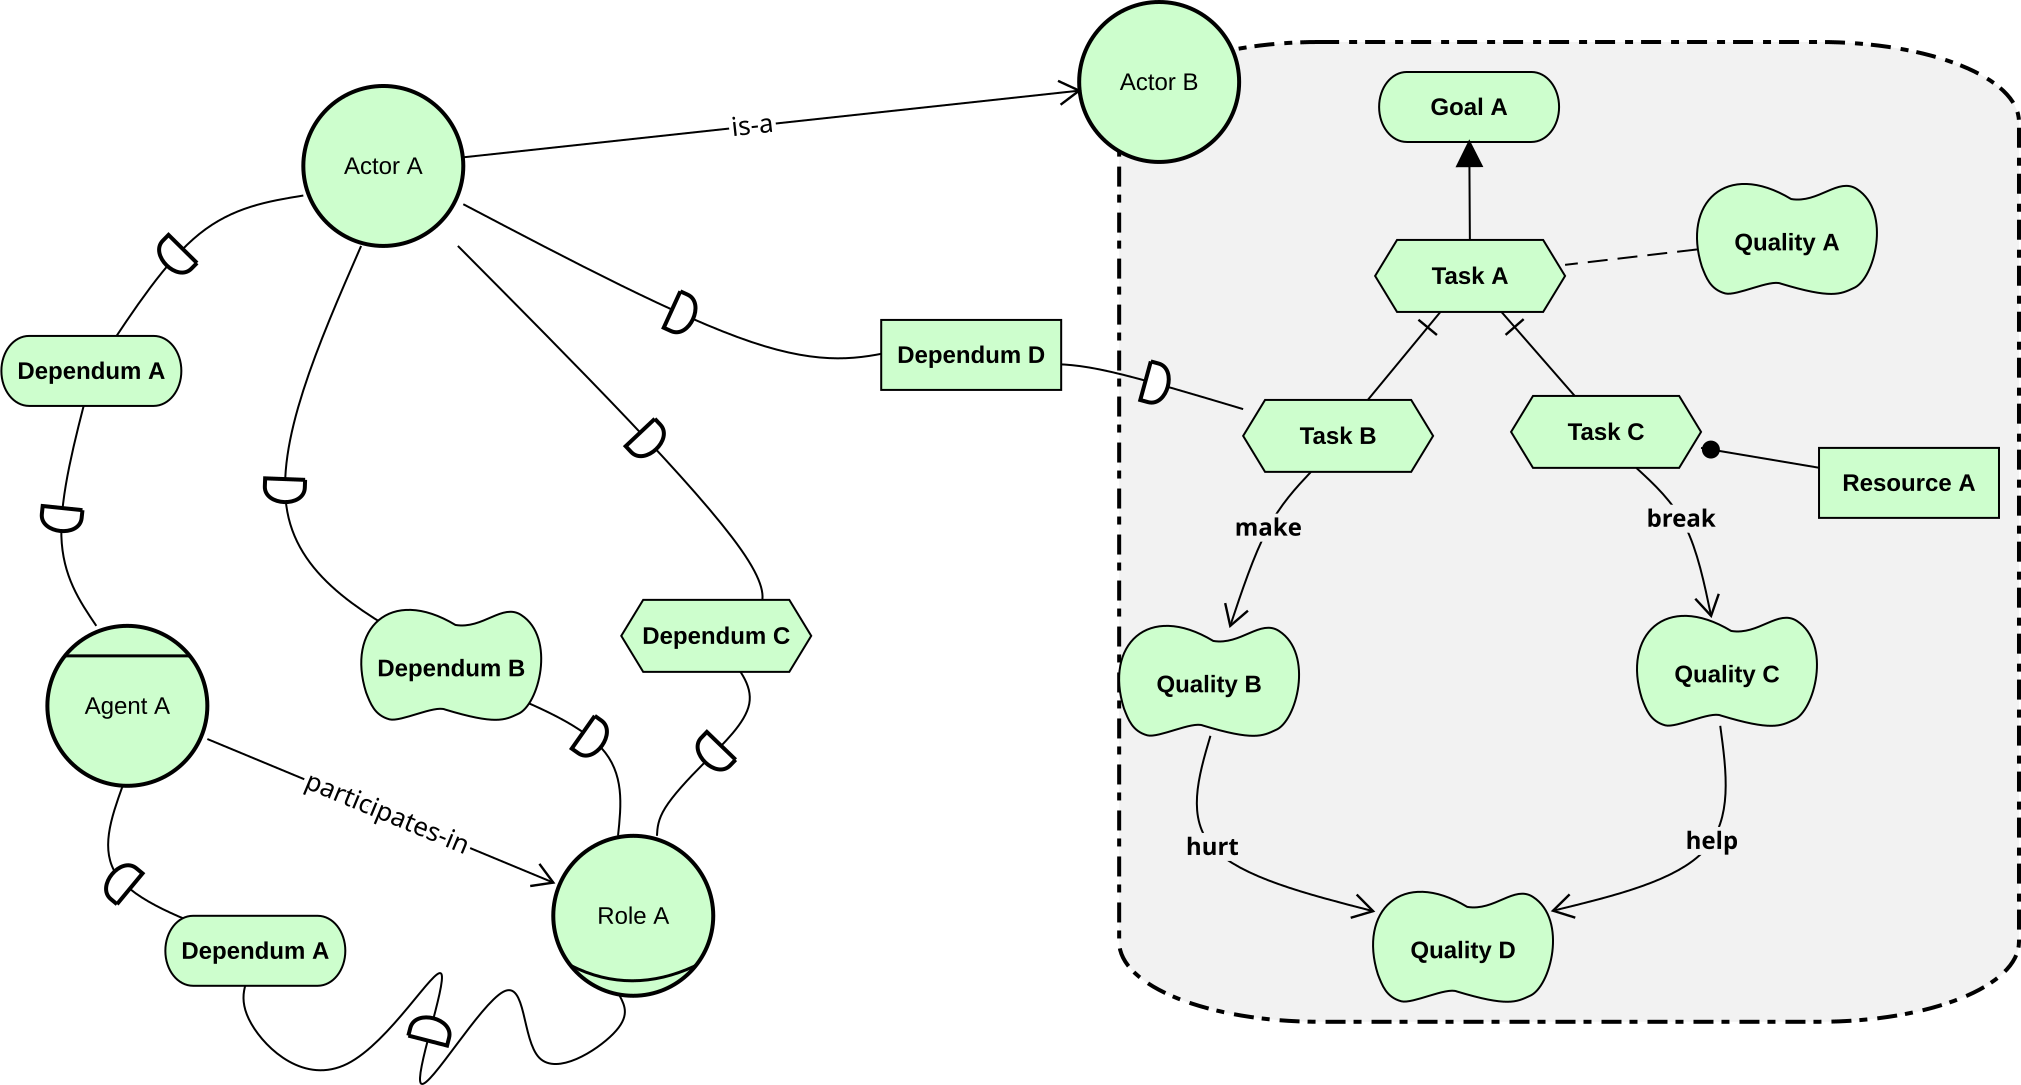
\includegraphics[width=6.063in,height=\textheight]{figures/fig-1-10.png}
\caption{Ký pháp iStar 2.0.}\label{fig:1-10}
\end{figure}

\thesisfigure{fig:1-10} xuất phát từ ví dụ ``Every iStar 2.0 element and link'' của piStar~\cite{ref-41}. Hình dạng của phần tử nằm giữa hai đầu phụ thuộc cho biết bên phụ thuộc cần kết quả thuộc kiểu nào. Chẳng hạn, Dependum D có hình chữ nhật của Resource, còn Dependum C có hình lục giác của Task.

\subsection{Refinement, Dependency và các quan hệ ý định}\label{sec:1-4-2}

Quan hệ is-a nối chủ thể cụ thể hơn với chủ thể tổng quát hơn, còn participates-in mô tả một chủ thể tham gia vào chủ thể khác, chẳng hạn một Agent đảm nhiệm một Role~\cite{ref-12}. Khi một chủ thể cần chủ thể khác cung cấp kết quả, mô hình dùng Dependency với tối đa năm thành phần. Depender là bên cần kết quả, dependee là bên được trông cậy, còn dependum mô tả tài nguyên, công việc, trạng thái hoặc đặc tính chất lượng cần được cung cấp~\cite{ref-12}. Mỗi đầu phụ thuộc cũng có thể chỉ tới một phần tử ý định của chủ thể tương ứng qua dependerElmt hoặc dependeeElmt~\cite{ref-42}.

Refinement liên kết Goal hoặc Task con với Goal hoặc Task cha trong cùng phạm vi chủ thể. Với AND-refinement, mọi phần tử con đều phải được thỏa mãn. OR-refinement yêu cầu ít nhất một phần tử con được thỏa mãn và cho phép nhiều phương án đạt đồng thời~\cite{ref-12}. Mỗi phần tử cha dùng một loại tinh chỉnh cho nhóm con trực tiếp. Nhánh AND có dấu gạch ngang gần phần tử cha, còn nhánh OR có đầu mũi tên hướng về cha~\cite{ref-12}.

Có thể diễn đạt hai quy tắc refinement trong~\cite{ref-12} bằng phép toán Boolean. Gọi \(p\) là phần tử cha đang xét, \(C(p)\) là tập các phần tử con trực tiếp và \(s(x)\) là mệnh đề ``phần tử \(x\) được thỏa mãn''. Trong cách diễn giải hai giá trị, điều kiện thỏa mãn \(p\) do từng loại refinement xác định như sau.

\[\text{AND:}\quad s(p)\  \Leftrightarrow \ \bigwedge_{c \in C(p)}s(c)\]

\[\text{OR:}\quad s(p)\  \Leftrightarrow \ \bigvee_{c \in C(p)}s(c)\]

NeededBy nối Resource với Task cần tài nguyên đó, còn Qualification nối Quality với Goal, Task hoặc Resource mà Quality mô tả~\cite{ref-12}. Khi mục đích là so sánh ảnh hưởng của các phương án lên một đặc tính chất lượng, mô hình dùng Contribution với đầu đích là Quality. Bốn nhãn make, help, hurt và break lần lượt biểu thị tác động tích cực đủ để đạt, tác động hỗ trợ, tác động cản trở và tác động tiêu cực đủ để phá vỡ đặc tính đó~\cite{ref-12}.

\subsection{Góc nhìn và phân tích mô hình iStar}\label{sec:1-4-3}

Có thể đọc mô hình từ các quan hệ giữa chủ thể trước, rồi xem các ý định trong từng đường bao. Góc nhìn thứ nhất cho biết mỗi bên cần kết quả gì từ bên nào. Góc nhìn thứ hai giải thích cách phân rã mục tiêu, tài nguyên cần có và tác động của từng phương án lên các Quality~\cite{ref-12}.

\begin{figure}
\centering
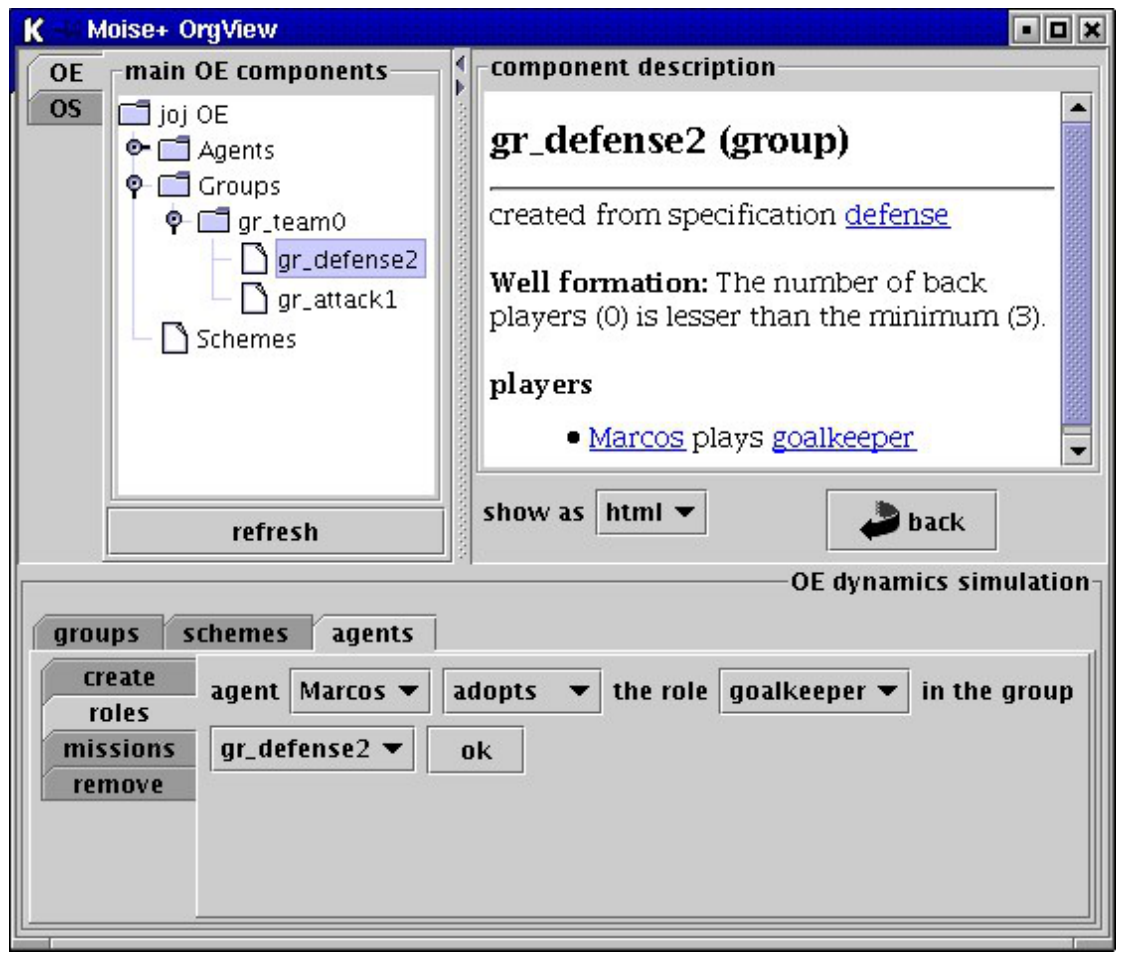
\includegraphics[width=6.063in,height=\textheight]{figures/fig-1-11.png}
\caption{Mô hình University Travel Reimbursement.}\label{fig:1-11}
\end{figure}

\thesisfigure{fig:1-11} lấy ví dụ University Travel Reimbursement của iStar 2.0 Language Guide~\cite{ref-12} và được xuất từ mô hình do piStar cung cấp~\cite{ref-41}. Student là vai trò trung tâm, PhD student chuyên biệt hóa Student và tác tử Mike White tham gia với vai trò PhD student. Trong đường bao của Student, Travel organized dùng hai nhánh AND là Authorization obtained và Trip booked, nên việc đặt chuyến đi chỉ đáp ứng một phần của mục tiêu này~\cite{ref-12}. Nhánh Trip booked dùng OR-refinement để sinh viên chọn giữa đặt từng phần (Trip parts booked) và đặt theo gói (Bundle booked). Nếu tự đặt vé, sinh viên cần tài nguyên Credit card cho tác vụ Pay for tickets theo liên kết NeededBy. Nếu điền biểu mẫu trực tuyến, sinh viên còn phụ thuộc vào hệ thống quản lý chuyến đi của trường để đạt Online form processed~\cite{ref-12}.

Mô hình cũng cho phép so sánh các phương án theo đặc tính chất lượng. Fill in online form có quan hệ help với No errors, còn Fill in paper form có quan hệ hurt với cùng đặc tính~\cite{ref-41}. Hai cách điền đều góp phần đạt Request prepared, nhưng mô hình ghi nhận tác động khác nhau lên khả năng tránh lỗi. Việc đọc đồng thời Refinement, Dependency và Contribution cho phép giải thích lựa chọn theo mục tiêu, sự phối hợp với chủ thể khác và chất lượng mong muốn~\cite{ref-12}.

\section{UML, OCL và công cụ USE}\label{sec:1-5}

UML cung cấp ký pháp mô tả cấu trúc và hành vi của mô hình \cite{ref-14}. Để kiểm tra các điều kiện trên cấu trúc đó, OCL dùng các biểu thức có kiểu để phát biểu ràng buộc và truy vấn \cite{ref-15}. Những biểu thức này có thể được đánh giá trên trạng thái đối tượng cụ thể trong USE \cite{ref-4}.

\subsection{Mô hình lớp, đối tượng và trạng thái}\label{sec:1-5-1}

Mô hình lớp xác định kiểu đối tượng, thuộc tính, thao tác, liên kết được phép và bội số tại các đầu liên kết~\cite{ref-14}. Trạng thái đối tượng cho biết những thể hiện nào đang tồn tại, giá trị thuộc tính của từng thể hiện và cách chúng liên kết với nhau. Một trạng thái hợp lệ phải phù hợp với kiểu và bội số đã khai báo, đồng thời thỏa các bất biến của mô hình~\cite{ref-4}.

\begin{figure}
\centering
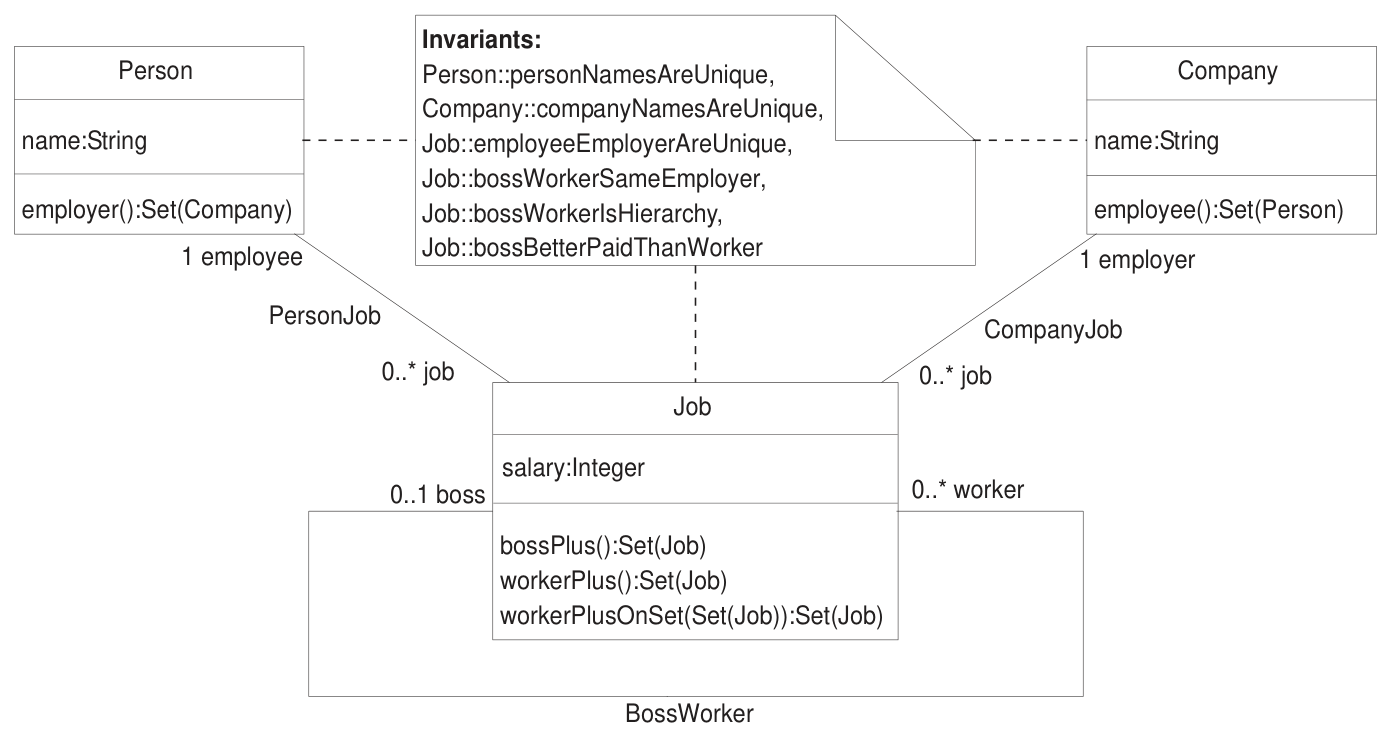
\includegraphics[width=5.7087in,height=\textheight]{figures/fig-1-12.png}
\caption{Biểu đồ lớp của mô hình việc làm.}\label{fig:1-12}
\end{figure}

Mô hình việc làm ở \thesisfigure{fig:1-12}~\cite{ref-16} gồm ba lớp Person, Company và Job. Mỗi Job gắn một công việc cụ thể với người lao động và công ty, còn liên kết BossWorker biểu diễn quan hệ cấp trên và cấp dưới giữa các công việc.

\begin{figure}
\centering
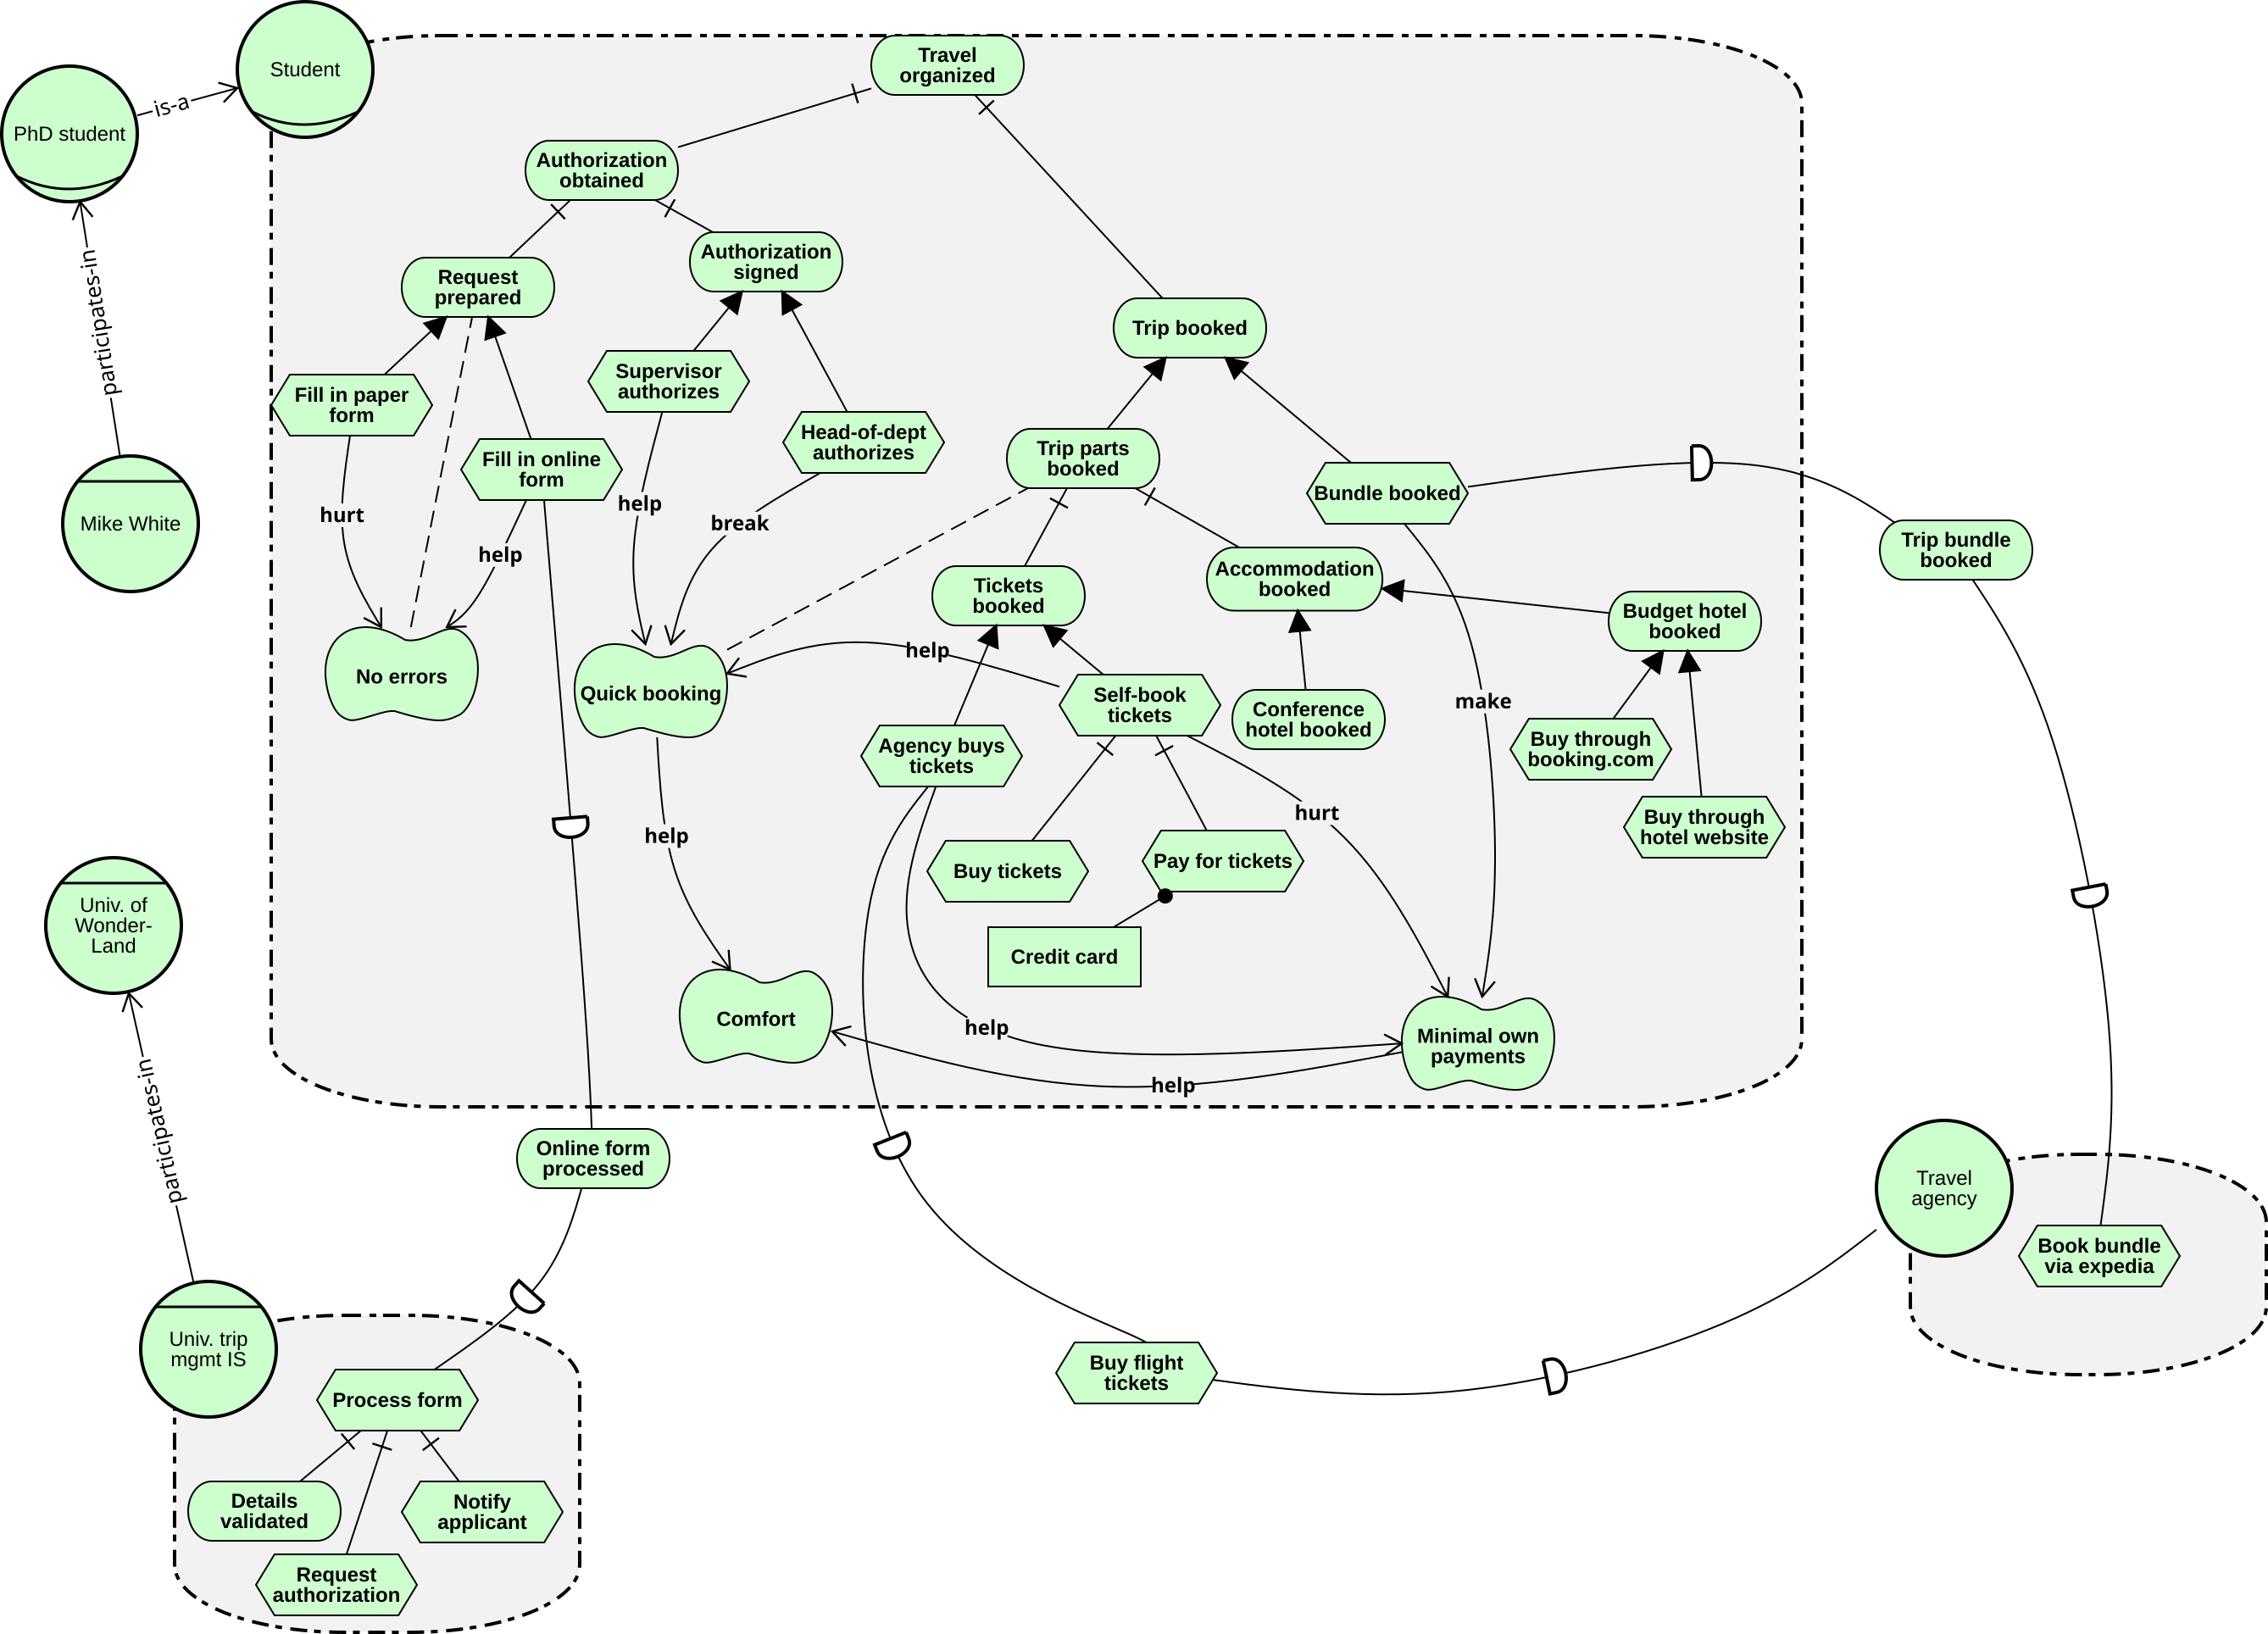
\includegraphics[width=4.9606in,height=\textheight]{figures/fig-1-13.png}
\caption{Trạng thái đối tượng của mô hình việc làm.}\label{fig:1-13}
\end{figure}

\thesisfigure{fig:1-13} cho thấy một trạng thái của mô hình việc làm được tạo từ tệp twoRoleTC.cmd~\cite{ref-16}. Cher làm việc tại hai công ty, nên mỗi công việc được ghi bằng một đối tượng Job có định danh và mức lương riêng.

\subsection{OCL và các loại ràng buộc}\label{sec:1-5-2}

OCL là ngôn ngữ biểu thức khai báo có kiểu, với phép đánh giá không gây tác dụng phụ. Ngữ cảnh cho biết biểu thức áp dụng cho kiểu đối tượng hay thao tác nào và từ khóa self tham chiếu tới đối tượng nào~\cite{ref-15}. Biểu thức có thể xét các tập hợp như Set, Bag và Sequence bằng phép lượng hóa hoặc truy vấn. Trong một trạng thái hợp lệ, bất biến của lớp phải đúng đối với từng đối tượng thuộc ngữ cảnh lớp đó~\cite{ref-15}.

\begin{samepage}

\thesisdisplaytitle{Đoạn mã 1.1}{Bất biến personNamesAreUnique}

\begin{Verbatim}
context p1:Person inv personNamesAreUnique:
Person.allInstances->forAll(p2|p1.name=p2.name implies p1=p2)
\end{Verbatim}

\end{samepage}

Đoạn mã 1.1 lấy bất biến personNamesAreUnique từ mô hình việc làm~\cite{ref-16}. Với mỗi p1, forAll xét mọi p2 thuộc lớp Person. Phép kéo theo yêu cầu p1 và p2 là cùng một đối tượng nếu tên của chúng trùng nhau, qua đó loại bỏ trường hợp hai người khác nhau có cùng tên.

Tiền điều kiện của một thao tác được xét trước khi thao tác thực hiện. Hậu điều kiện được xét trên kết quả thực hiện và có thể tham chiếu giá trị cũ qua @pre ở những vị trí được OCL cho phép \cite{ref-15}.

\begin{samepage}

\thesisdisplaytitle{Đoạn mã 1.2}{Hợp đồng của thao tác marry}

\begin{Verbatim}
marry(aSpouse:Person)
pre isUnmarried: civstat<>#married
post isMarried: civstat=#married
\end{Verbatim}

\end{samepage}

Đoạn mã 1.2 trích hai ràng buộc của thao tác marry từ đặc tả~\cite{ref-4}. Tiền điều kiện isUnmarried kiểm tra tình trạng hôn nhân trước thao tác, còn hậu điều kiện isMarried yêu cầu tình trạng sau thao tác là married. Đặc tả đầy đủ còn đặt điều kiện đối với người phối ngẫu.

Trong OCL, false là giá trị Boolean, null cho biết giá trị vắng mặt và invalid biểu thị kết quả đánh giá không hợp lệ. Bất biến chỉ được thỏa khi biểu thức cho kết quả true~\cite{ref-15}. Sự phân biệt này cho phép bộ kiểm chứng ghi nhận riêng kết quả sai và trường hợp không thể đánh giá điều kiện.

\subsection{Môi trường USE và khả năng mở rộng}\label{sec:1-5-3}

USE (UML-based Specification Environment) hỗ trợ nạp mô hình lớp UML/OCL, xây dựng trạng thái đối tượng và đánh giá biểu thức trên trạng thái đó~\cite{ref-4}.

\begin{figure}
\centering
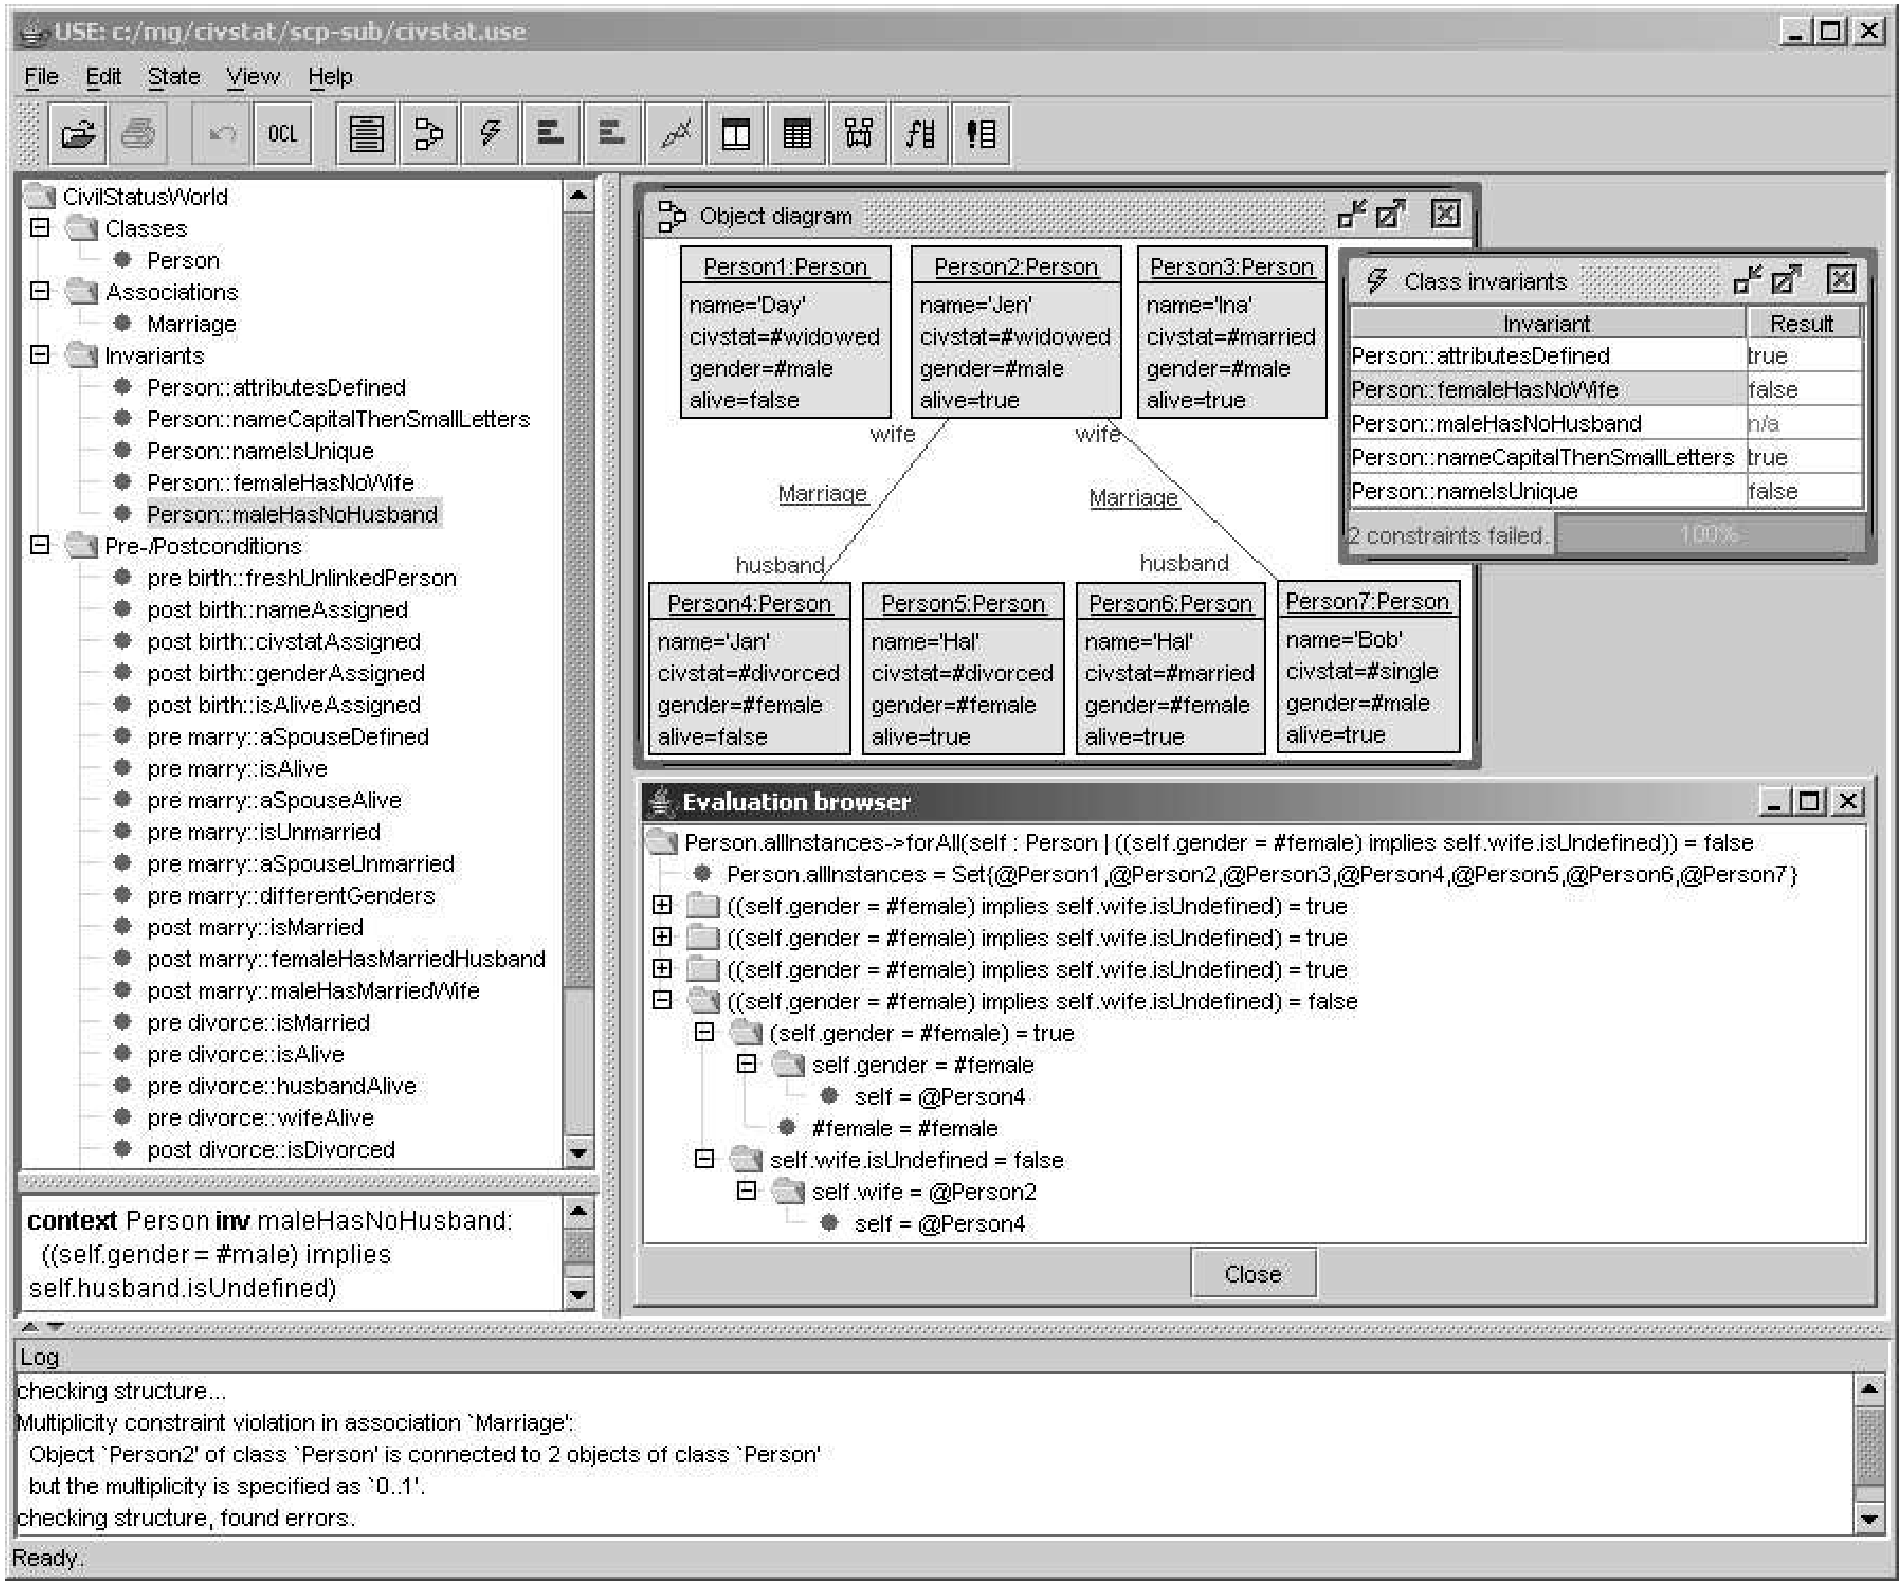
\includegraphics[width=6.0236in,height=\textheight]{figures/fig-1-14.png}
\caption{Trạng thái đối tượng và kết quả OCL trong USE.}\label{fig:1-14}
\end{figure}

\thesisfigure{fig:1-14} minh họa cách USE trình bày dữ liệu và kết quả kiểm tra~\cite{ref-4}. Biểu đồ đối tượng cho thấy dữ liệu trạng thái, Class Invariants liệt kê kết quả kiểm tra và Evaluation Browser cho phép xem từng giá trị tham gia đánh giá biểu thức.

Sinh trạng thái trong USE hỗ trợ khảo sát tính nhất quán và tính độc lập của các bất biến~\cite{ref-16}. Cho \(M\) là một mô hình lớp, \(Inst(M)\) là tập các trạng thái phù hợp với cấu trúc của \(M\), và \(\Phi\) là tập bất biến. Tính nhất quán có thể được chứng minh bằng một trạng thái làm chứng \(s \in Inst(M)\) sao cho \(s \vDash \Phi\). Để kiểm tra tính độc lập của bất biến \(\varphi \in \Phi\), gọi \(\Psi\) là tập các bất biến còn lại sau khi bỏ \(\varphi\). Một trạng thái thỏa mãn \(\Psi\) nhưng bác bỏ \(\varphi\) là bằng chứng cho thấy \(\varphi\) độc lập với các bất biến còn lại~\cite{ref-4}.

\[\exists s \in Inst(M):\quad s \vDash \Psi\quad \land \quad s \vDash \neg\varphi.\]

Khi việc sinh trạng thái giới hạn số thể hiện hoặc miền giá trị, kết luận về sự vắng mặt của một trạng thái làm chứng chỉ có hiệu lực trong miền được khảo sát, trừ trường hợp có lập luận bao quát miền còn lại~\cite{ref-16}. USE còn cung cấp cơ chế mở rộng qua plugin, cho phép các công cụ bổ sung chức năng làm việc với mô hình và trạng thái~\cite{ref-17}.

\section{Kiểm chứng hệ thống đa tác tử}\label{sec:1-6}

Kiểm chứng mô hình (model checking) xem xét hành vi của hệ thống thông qua một mô hình chuyển trạng thái. Trong hệ đa tác tử, cách mô hình hóa lịch thực thi ảnh hưởng đến những hành vi được xét~\cite{ref-19}. Kiểm chứng khi thực thi (runtime verification) rút kết luận từ vết của một lần chạy cụ thể~\cite{ref-5}. Vì vậy, dữ kiện môi trường nằm ngoài phạm vi quan sát có thể làm giới hạn kết luận của bộ kiểm chứng~\cite{ref-23}.

\subsection{Kiểm chứng mô hình (Model Checking)}\label{sec:1-6-1}

Một cách biểu diễn hệ chuyển trạng thái là cấu trúc Kripke \(K = \left( S,S_{0},R,L \right)\). Trong đó \(S\) là tập trạng thái, \(S_{0}\) là tập trạng thái khởi đầu, \(R \subseteq S \times S\) là quan hệ chuyển và \(L\) gán cho mỗi trạng thái tập mệnh đề nguyên tử đúng tại trạng thái đó~\cite{ref-19}. Với một công thức thuộc tính \(\varphi\), ký hiệu \(K \vDash \varphi\) diễn tả rằng mô hình thỏa mãn \(\varphi\) theo ngữ nghĩa của logic được sử dụng. Kết luận được xác định trên các trạng thái khởi đầu và các hành vi của chính mô hình~\cite{ref-19}.

Khi thuộc tính an toàn được phát biểu bằng một điều kiện luôn phải đúng, đường đi từ trạng thái khởi đầu đến trạng thái vi phạm là một phản ví dụ~\cite{ref-19}. Với tính chất thời gian hoặc chiến lược, bằng chứng cần thiết còn phụ thuộc vào logic và thuật toán kiểm tra. Chẳng hạn, MCMAS dùng interpreted systems để biểu diễn hệ đa tác tử và kiểm tra thuộc tính về thời gian, tri thức hoặc chiến lược~\cite{ref-20}. Phạm vi kết luận do mức trừu tượng và không gian trạng thái được kiểm tra quyết định~\cite{ref-22}.

\subsection{Kiểm chứng khi thực thi (Runtime Verification)}\label{sec:1-6-2}

Trong runtime verification, bộ giám sát đánh giá một đặc tả trên vết thực thi quan sát được~\cite{ref-5}. Với ngữ nghĩa ba giá trị cho một tiền tố hữu hạn \(u\) của vết, kết quả phụ thuộc vào các phần tiếp nối có thể có. Công thức \(\varphi\) nhận giá trị đúng nếu mọi phần tiếp nối vô hạn của \(u\) đều thỏa mãn \(\varphi\). Công thức nhận giá trị sai nếu không có phần tiếp nối nào thỏa mãn. Kết quả chưa xác định khi tồn tại cả hai loại phần tiếp nối~\cite{ref-18}.

Một tính chất an toàn yêu cầu sự kiện xấu không bao giờ xuất hiện. Khi tiền tố đã chứa sự kiện xấu cụ thể, mọi phần tiếp nối đều giữ sự kiện đó, nên bộ giám sát có thể kết luận vi phạm. Với yêu cầu một phản hồi cuối cùng phải xuất hiện, việc chưa thấy phản hồi trong tiền tố vẫn để ngỏ khả năng có phản hồi ở phần tiếp nối~\cite{ref-18}. Vết quan sát thiếu sự kiện hoặc chứa dữ liệu sai cũng là nguồn gây bất định~\cite{ref-23}.

\subsection{Trace, snapshot và checkpoint}\label{sec:1-6-3}

Vết thực thi (trace) là chuỗi sự kiện hoặc trạng thái có thứ tự~\cite{ref-5}, còn ảnh chụp trạng thái (snapshot) ghi thông tin tại một mốc quan sát~\cite{ref-21}. Trong phương pháp ở Mục 2.6.2, checkpoint xác định ranh giới thu thập dữ liệu và nhận quyết định kiểm chứng. Một dãy snapshot có thể dùng làm vết trạng thái, và những gì có thể kết luận phụ thuộc vào dữ kiện ghi được trong dãy đó~\cite{ref-23}.

Hai lần quan sát liên tiếp có thể cho cùng giá trị của một thuộc tính mặc dù thuộc tính đó đã thay đổi trong khoảng giữa. Vì vậy, một bất biến đúng ở mọi snapshot quan sát được cung cấp bằng chứng tại những mốc đã quan sát~\cite{ref-23}. Để kết luận về toàn bộ diễn biến, cần có thêm giả thiết hoặc bằng chứng về các trạng thái trung gian~\cite{ref-5}.

Đối với hệ phân tán, tính nhất quán của ảnh chụp toàn cục phụ thuộc cả vào trạng thái tiến trình lẫn thông điệp đang truyền. Thuật toán của Chandy và Lamport ghi nhận cả hai thành phần~\cite{ref-21}. Khi dùng ảnh chụp để kiểm chứng, còn phải xét các mốc quan sát có cung cấp đủ dữ liệu cho tính chất đang được đánh giá hay không~\cite{ref-23}.

\section{Các nghiên cứu liên quan}\label{sec:1-7}

Trong nghiên cứu về USE, việc kiểm tra một trạng thái cụ thể cho biết bất biến nào được thỏa~\cite{ref-4}. Sinh trạng thái mở rộng khả năng này bằng cách tìm trường hợp làm chứng hoặc phản ví dụ trong phạm vi đã chọn~\cite{ref-16}. Với đặc tả hướng mục tiêu, iStar 2.0 cung cấp ký pháp mô tả chủ thể, ý định và các phương án đáp ứng~\cite{ref-12}. Công cụ piStar cho phép xây dựng và kiểm tra cấu trúc biểu đồ theo ký pháp đó trước khi xét dữ liệu thực thi~\cite{ref-41}.

Đối với hệ đa tác tử, các công trình model checking xét thuộc tính trên mô hình hoặc chương trình tác tử được biểu diễn dưới dạng thích hợp~\cite{ref-22}. RV4JaCa đưa giám sát giao thức tương tác vào JaCaMo và đánh giá trao đổi quan sát được trong phiên thực thi~\cite{ref-24}. Hướng kết hợp kiểm chứng mô hình và kiểm chứng khi thực thi khai thác các loại bằng chứng khác nhau để phân tích tính chất của hệ đa tác tử~\cite{ref-25}.

Các công trình vừa khảo sát dùng những loại bằng chứng khác nhau, từ trạng thái đối tượng đến mô hình ý định và vết tương tác. Nghiên cứu kết nối những cách tiếp cận này bằng cách dựng trạng thái đối tượng trong USE từ dữ liệu JaCaMo. Trạng thái đó vừa dùng để kiểm tra ràng buộc, vừa cung cấp dữ liệu cho việc đánh giá mục tiêu (Mục 2.3).

\section{Tổng kết chương}\label{sec:1-8}

Phân biệt cú pháp cụ thể, cấu trúc mô hình và ngữ nghĩa giúp xác định một đặc tả có hợp lệ và được diễn giải trên trạng thái nào. Trên nền JaCaMo, cần xác định dữ liệu nào thuộc về tác tử, môi trường và tổ chức trước khi dùng UML và OCL để mô tả trạng thái và ràng buộc. iStar bổ sung góc nhìn về mục tiêu và cách các chủ thể phối hợp để đạt mục tiêu đó.

Vết thực thi, snapshot và checkpoint giúp phân biệt diễn biến của chương trình với phần dữ liệu được ghi nhận khi kiểm chứng. Phạm vi kết luận phụ thuộc vào những dữ kiện mà bộ giám sát có thể quan sát~\cite{ref-23}. Chương 2 vận dụng sự phân biệt này để kiểm tra ràng buộc và đánh giá tiến độ thực hiện mục tiêu trên JaCaMo.

\chapter{PHƯƠNG PHÁP ĐẶC TẢ VÀ KIỂM CHỨNG HỆ THỐNG ĐA TÁC TỬ TRÊN USE}\label{sec:2}

Phương pháp kiểm chứng trên USE mô tả cùng một hệ thống JaCaMo từ hai góc nhìn. Góc nhìn trạng thái hệ thống (System State) ghi nhận các đối tượng, giá trị và quan hệ hiện có, còn góc nhìn hướng mục tiêu (Goal-Oriented) cho biết các mục tiêu và nhiệm vụ cần đánh giá. Ở mỗi checkpoint, trạng thái CSL cung cấp dữ liệu để liên kết hai góc nhìn.

\section{Giới thiệu}\label{sec:2-1}

Nghiên cứu tiếp thu cách dùng chung trạng thái từ công trình ``On Checking the Conformance between iStar and BPMN Models''~\cite{ref-28}. Công trình biểu diễn dữ liệu tổ chức và dữ liệu miền bằng CSL, rồi đánh giá các điều kiện OCL của iStar trên trạng thái sinh từ kịch bản BPMN. Phương pháp trong chương này giữ cách đánh giá dựa trên trạng thái chung và áp dụng nó cho chuỗi trạng thái quan sát được từ chương trình JaCaMo đang chạy.

Mục tiêu của phương pháp là kiểm tra trạng thái JaCaMo, theo dõi tiến độ Goal và Task, rồi quyết định việc thực thi có thể tiếp tục từ checkpoint đang xét hay cần giữ dừng. Phần động cơ đặt bài toán qua một tình huống thực tế. Phần tổng quan xác định bốn bước và kết quả của từng bước trước khi trình bày chi tiết.

\section{Động cơ nghiên cứu (Motivation)}\label{sec:2-2}

Trong hệ thống đa tác tử, mỗi tác tử có thể chọn hành động dựa trên thông tin cục bộ \cite{ref-1}. Trong JaCaMo, các tác tử trao đổi thông điệp, thao tác trên artifact dùng chung và đảm nhiệm vai trò trong tổ chức. Các hoạt động có thể xen kẽ và làm thay đổi trạng thái ở nhiều thành phần \cite{ref-2}. Vì vậy, kết quả thành công của một thao tác chỉ cung cấp một phần bằng chứng về trạng thái và tiến độ chung của hệ thống.

Các công trình trước đã kiểm tra những loại bằng chứng khác nhau trong hệ đa tác tử. Bordini và cộng sự xét các diễn biến có thể có trong mô hình chương trình~\cite{ref-19}, còn RV4JaCa kiểm tra giao thức từ thông điệp thu trong một lần chạy~\cite{ref-24}. Ở mức mô hình đặc tả, USE dùng trạng thái đối tượng để đánh giá ràng buộc OCL~\cite{ref-4}, trong khi iStar biểu diễn mục tiêu, nhiệm vụ và các quan hệ ý định~\cite{ref-12}.

Một chuỗi thông điệp đúng giao thức vẫn có thể thiếu dữ kiện về thuộc tính của artifact, vai trò đang được đảm nhiệm và tiến độ thực hiện nhiệm vụ. Việc thỏa bất biến tại một thời điểm cũng chưa đủ để kết luận một nhiệm vụ đã hoàn thành~\cite{ref-28}. Vì vậy, bộ kiểm chứng cần nối dữ liệu JaCaMo với đúng đối tượng và liên kết CSL qua các lần quan sát, đồng thời phân biệt trường hợp thiếu bằng chứng với vi phạm đã xác định~\cite{ref-23}.

\subsection{Ví dụ Auction}\label{sec:2-2-1}

Auction chạy hai phiên đấu giá a1 và a2 đồng thời. Tại checkpoint 39, cả hai đang chờ mức giá tốt hơn. Đến checkpoint 42, chỉ a2 nhận được giá tốt hơn. Các bất biến đều đạt ở hai mốc và JaCaMo được phép tiếp tục. Kết quả của mỗi phiên được theo dõi riêng (Mục 3.5.1).

Trong một ca thử khác, giá tăng từ 10 lên 20. Các bất biến vẫn đạt nhưng mục tiêu giữ giá không tăng đã bị vi phạm, nên JaCaMo nhận quyết định giữ dừng (\thesisfigure{fig:3-8}). Quyết định vì vậy phụ thuộc cả vào trạng thái hiện tại và diễn biến của từng phiên.

\section{Tổng quan phương pháp (Method Overview)}\label{sec:2-3}

Phương pháp gồm bốn bước, bắt đầu bằng việc xác định mô hình và điều kiện kiểm chứng trước khi chạy JaCaMo. Đặc tả CSL mô tả dữ liệu nghiệp vụ và cấu trúc tổ chức thông qua các kiểu đối tượng, thuộc tính, liên kết và bất biến. USE biên dịch đặc tả này thành mô hình cấu trúc dùng chung cho ánh xạ và kiểm chứng (Mục 2.4). Trên các kiểu ngữ cảnh CSL đã xác định, đặc tả iStar mở rộng gắn điều kiện OCL cho Goal và Task. Kiểu mục tiêu cùng các điều kiện này cho biết cần quan sát dữ liệu nào để đánh giá tiến độ của từng đối tượng (Mục 2.5). Luật XML dùng để đưa dữ liệu JaCaMo vào cấu trúc đã khai báo cũng được chuẩn bị trước khi khởi chạy.

Hai bước còn lại được thực hiện tại mỗi checkpoint. Khi có ảnh chụp trạng thái JaCaMo, bộ ánh xạ dùng luật XML để gán giá trị thuộc tính và dùng dữ liệu cấu trúc từ ảnh để dựng các liên kết tương ứng. Nếu cập nhật thành công, kết quả là cặp trạng thái CSL trước và sau lần cập nhật (Mục 2.6). Từ đó, USE kiểm tra bất biến trên trạng thái hiện tại và đánh giá Goal, Task dựa trên các điều kiện cùng lịch sử của từng ngữ cảnh. Công cụ tổng hợp kết quả để phản hồi về đúng checkpoint. Dữ liệu thiếu hoặc lỗi phép chiếu dẫn đến giữ dừng vì chưa đủ căn cứ kiểm chứng (Mục 2.7).

\section{Đặc tả CSL trong USE}\label{sec:2-4}

Một mô hình mục tiêu mô tả kết quả mà các chủ thể mong muốn, còn mô hình quy trình mô tả hoạt động có thể dẫn tới kết quả đó. Để đánh giá cả hai trên cùng dữ liệu, Nguyen và cộng sự xây dựng CSL (Composite State Language) nhằm biểu diễn trạng thái nghiệp vụ và cấu trúc tổ chức trong một mô hình chung~\cite{ref-28}. CSL mở rộng cách dùng mô hình lớp UML bằng việc đưa ngữ cảnh tổ chức và vai trò vào đặc tả. Nhờ đó, trạng thái cho biết chủ thể nào đảm nhiệm vai trò nào bên cạnh những giá trị nghiệp vụ đang có. Các điều kiện của iStar và BPMN có thể tham chiếu chung trạng thái này dù hai mô hình được xây dựng độc lập~\cite{ref-28}.

\begin{figure}
\centering
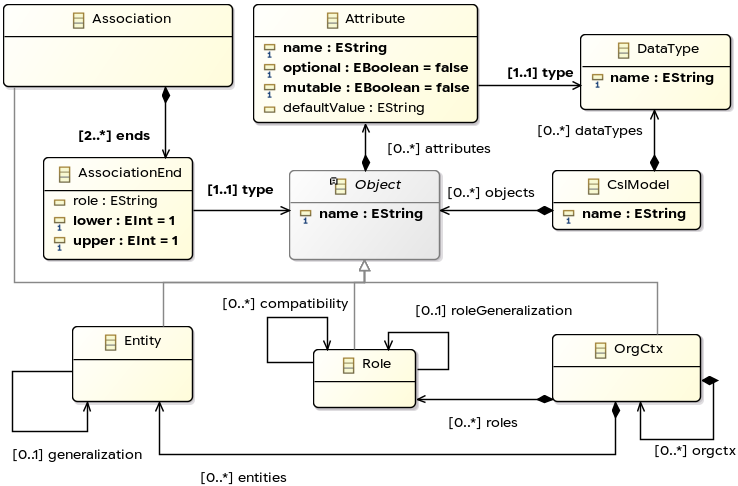
\includegraphics[width=4.6063in,height=\textheight]{figures/fig-2-1.png}
\caption{Siêu mô hình CSL.}\label{fig:2-1}
\end{figure}

Trong siêu mô hình CSL ở \thesisfigure{fig:2-1}~\cite{ref-28}, CslModel tập hợp các khai báo Object và DataType. Object là lớp trừu tượng có tên và danh sách thuộc tính, với bốn chuyên biệt Entity, Role, OrgCtx và Association. Những khai báo này xác định cấu trúc được phép của mô hình, còn các đối tượng cụ thể xuất hiện trong từng trạng thái của mô hình~\cite{ref-28}.

\begin{quote}
Entity mô tả thực thể nghiệp vụ thụ động. Quan hệ generalization có bội số 0..1, nên mỗi kiểu Entity có tối đa một kiểu tổng quát trực tiếp. Phạm vi tổ chức được xác định bởi OrgCtx, có thể chứa các Entity, Role và OrgCtx con với bội số 0..* cho mỗi quan hệ chứa~\cite{ref-28}. Khi thực thi, một tác tử hoặc một thể hiện OrgCtx có thể đảm nhiệm Role trong một ngữ cảnh cụ thể. Nếu vai trò có trạng thái riêng, dữ liệu đó thuộc về thể hiện vai trò. Quan hệ roleGeneralization cho phép tối đa một vai trò cha, còn compatibility xác định những vai trò mà cùng một chủ thể có thể đảm nhiệm đồng thời~\cite{ref-28}.

Cấu trúc của trạng thái còn phụ thuộc vào các liên kết và thuộc tính được khai báo. Mỗi Association có ít nhất hai AssociationEnd, mỗi đầu chỉ tới đúng một kiểu Object và có thể có tên điều hướng role. Cận dưới lower và cận trên upper đều mặc định bằng 1. Tên điều hướng xác định đầu liên kết, trong khi Role xác định vị trí trong tổ chức~\cite{ref-28}. Đối với dữ liệu trên đối tượng, mỗi Attribute có tên và đúng một kiểu DataType. Hai cờ optional và mutable lần lượt cho phép giá trị vắng mặt hoặc thay đổi, mặc định đều bằng false, còn defaultValue lưu biểu diễn của giá trị mặc định nếu có~\cite{ref-28}.
\end{quote}

\begin{samepage}

\thesisdisplaytitle{Định nghĩa 2.1}{Mô hình CSL}

\[S = \langle O_{S},L_{S},\Phi,H\rangle,\quad L_{S} \subseteq O_{S} \times O_{S}.\]

\end{samepage}

Trong biểu diễn hình thức của CSL~\cite{ref-28}, O\_S là tập các đối tượng CSL có kiểu, L\_S là các quan hệ cấu trúc và \(\Phi\) là tập ràng buộc OCL. Thành phần H nối các khai báo tổ chức trong CSL với các phần tử ở hai mô hình được tích hợp. Khi kết hợp iStar với BPMN, mỗi Pool tương ứng với đúng một kiểu OrgCtx, còn mỗi Actor của iStar hoặc Lane của BPMN tương ứng với đúng một kiểu Role~\cite{ref-28}.

Trạng thái \(\sigma\) của một mô hình CSL ghi các thể hiện đang tồn tại, giá trị thuộc tính, liên kết và việc đảm nhiệm vai trò. Trong công trình của Nguyen và cộng sự, các trạng thái đưa vào kịch bản phải thỏa mọi ràng buộc trong \(\Phi\), ký hiệu \(\sigma\) \(\vDash\) \(\Phi\)~\cite{ref-28}. Khi kiểm chứng JaCaMo, bộ thu có thể ghi lại cả trạng thái vi phạm \(\Phi\). Một mô hình CSL vì vậy được dùng để đánh giá lần lượt nhiều ảnh chụp từ thực thi.

Khi nạp đặc tả CSL vào USE, CslFrontend.compile đọc và kiểm tra mô hình. Sau bước này, CslModelCompiler.compile tạo các lớp, thuộc tính, liên kết và bất biến trong USE. CslContextSchema.installObservations bổ sung các liên kết để điều hướng từ một thực thể tới ngữ cảnh chứa nó hoặc tới tác tử đang quan sát nó. Mục 2.6 trình bày cách dựng các thể hiện từ dữ liệu JaCaMo. Mục 2.7 giải thích cách kiểm tra bất biến và đánh giá các điều kiện iStar trên trạng thái đã dựng.

\begin{figure}
\centering
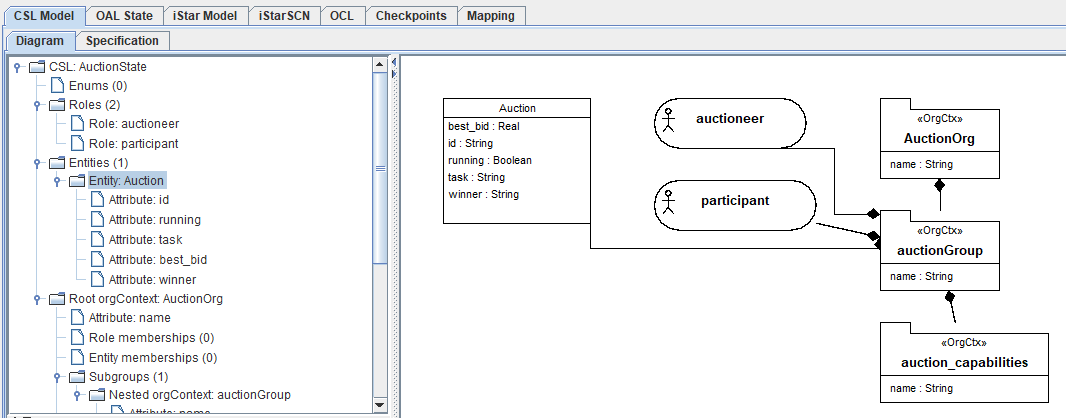
\includegraphics[width=6.09in,height=\textheight]{figures/fig-2-2.png}
\caption{Mô hình CSL của Auction.}\label{fig:2-2}
\end{figure}

\thesisfigure{fig:2-2} cho thấy AuctionOrg chứa ngữ cảnh auctionGroup, nơi khai báo hai vai trò auctioneer, participant và thực thể Auction. Các thuộc tính running, best\_bid và winner mô tả dữ liệu của từng phiên đấu giá. Để đọc mô hình trong thẻ CSL Model, có thể nhận ra Entity qua khung chữ nhật ghi «entity» và ngăn thuộc tính. OrgCtx dùng khung có tai ghi «OrgCtx», Role dùng khung bo tròn có biểu tượng người, còn kiểu liệt kê đặt các giá trị bên dưới tên. Trên các đường nối, tam giác rỗng chỉ kiểu tổng quát, hình thoi đặc chỉ hợp thành và hình thoi rỗng chỉ kết tập. Vòng tròn rỗng biểu thị quan hệ tương thích và ô vuông rỗng biểu thị sở hữu. Khả năng đảm nhiệm vai trò được vẽ bằng nét đứt có nhãn may enact. Các ký hiệu này diễn tả cấu trúc khai báo. Thẻ OAL State hiển thị các đối tượng và giá trị tại checkpoint mà những điều kiện iStar ở Mục 2.5 sử dụng.

\section{Đặc tả iStar mở rộng trong USE}\label{sec:2-5}

Trong iStar, quan hệ tinh chỉnh AND cho biết mục tiêu cha cần tất cả các nhánh con~\cite{ref-12}. Để đánh giá trong khi hệ thống chạy, cần đặc tả dữ kiện nào chứng minh từng nhánh đã đạt và kết quả ở một bước có hiệu lực thế nào ở các bước tiếp theo~\cite{ref-28}.

\begin{figure}
\centering
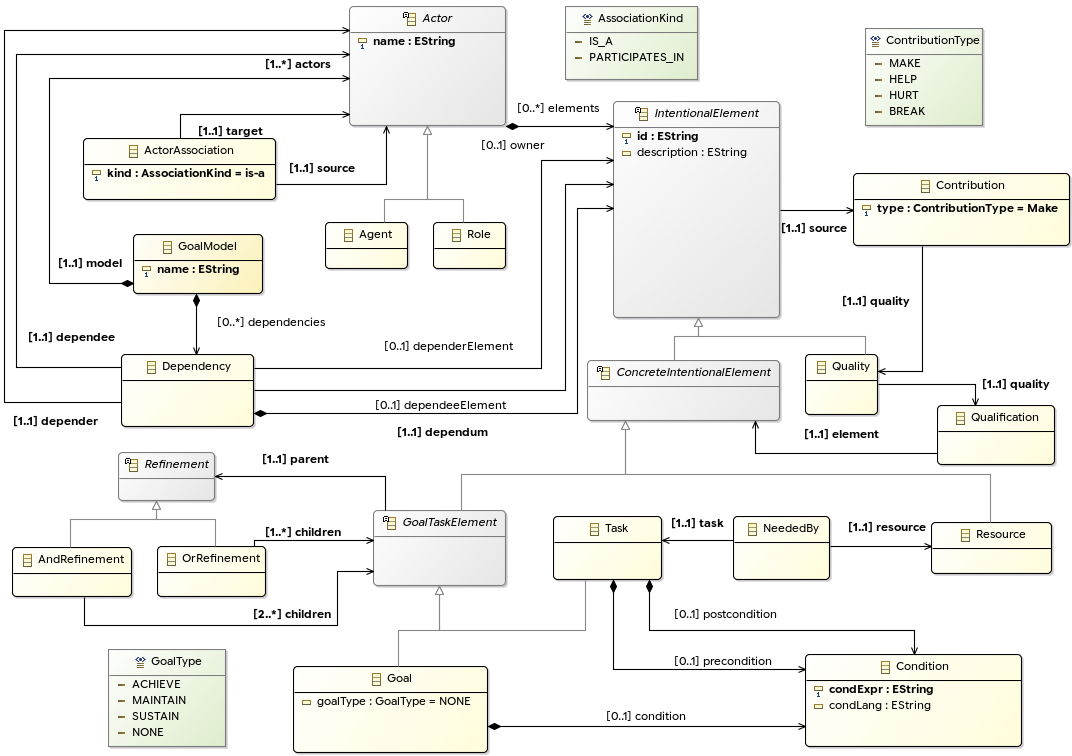
\includegraphics[width=5.1181in,height=\textheight]{figures/fig-2-3.png}
\caption{Siêu mô hình iStar mở rộng.}\label{fig:2-3}
\end{figure}

Bài báo bổ sung các điều kiện đọc trạng thái cho Goal và Task, đồng thời xác định cách diễn giải kết quả của Goal qua thời gian~\cite{ref-28}. \thesisfigure{fig:2-3} cho thấy lớp Condition, các liên kết condition, precondition và postcondition, cùng thuộc tính goalType.

Lớp Condition gắn bằng chứng quan sát với mục tiêu và nhiệm vụ qua hai trường condExpr và condLang. Một Goal có tối đa một condition, còn một Task có tối đa một precondition và một postcondition. Các biểu thức OCL có thể đọc thuộc tính và điều hướng qua liên kết trong trạng thái CSL. Bài báo dùng giá trị tiền điều kiện và hậu điều kiện để đánh giá Task tại một bước~\cite{ref-28}. Trong bộ kiểm chứng JaCaMo, SnapshotVerifier yêu cầu khai báo đúng một tiền điều kiện và một hậu điều kiện cho mỗi Task.

\begin{samepage}

\thesisdisplaytitle{Định nghĩa 2.2}{Mô hình iStar mở rộng}

\[G = \langle A,N,R,\tau,\kappa_{G}\rangle,\quad\tau:N \rightharpoonup T.\]

\end{samepage}

Mô hình iStar mở rộng trong~\cite{ref-28} dùng A làm tập chủ thể, N làm tập phần tử ý định có kiểu và R làm tập quan hệ. Thành phần \(\kappa\)\_G gắn đặc tả phụ thuộc trạng thái vào phần tử lá. Hàm bộ phận \(\tau\) gán kiểu thời gian cho Goal trong tập \{Achieve, Maintain, Sustain, None\}, với None là giá trị mặc định ở cấp siêu mô hình~\cite{ref-28}.

\begin{quote}
Các kiểu thời gian khác nhau ở cách sử dụng kết quả của những lần quan sát. Với Achieve, mục tiêu được ghi nhận sau lần đầu thấy điều kiện đúng và kết quả đạt được giữ lại dù giá trị thay đổi ở bước sau. Với Maintain, điều kiện phải được duy trì và lần quan sát sai được ghi nhớ như một vi phạm~\cite{ref-28}. Sustain cho phép chờ khi điều kiện ban đầu chưa đúng. Sau lần đầu điều kiện đúng, việc mất điều kiện được xem là vi phạm. Trường hợp None dùng kết quả tức thời hoặc kết quả lan truyền tại bước hiện tại~\cite{ref-28}.
\end{quote}

Tại bước i, giá trị của phần tử lá lấy từ điều kiện, còn giá trị của phần tử được suy ra lấy từ các nhánh tinh chỉnh hoặc quan hệ phụ thuộc. Sau khi áp dụng ngữ nghĩa thời gian, hàm đánh dấu \(\mu_{i}\) gán cho mỗi phần tử ý định x giá trị được đánh giá \(v_{i}\)(x) trong tập \{\(\bot\), ?, \(\top\)\}, lần lượt chỉ vi phạm, chưa xác định và đạt~\cite{ref-28}.

\[\Delta = \{\bot,?,\top\},\quad\quad\mu_{i}:N \rightarrow \Delta,\quad\quad\mu_{i}(x) = v_{i}(x).\]

Trong bài báo, Task có kết quả chưa xác định khi tiền điều kiện sai. Khi tiền điều kiện đúng, hậu điều kiện xác định kết quả đạt hay vi phạm tại bước đang xét~\cite{ref-28}. Bộ kiểm chứng JaCaMo tích lũy bằng chứng qua lịch sử và có thể ghi nhận tiền điều kiện ở một checkpoint rồi ghi nhận hậu điều kiện tại một checkpoint sau. Nếu mới ghi nhận tiền điều kiện mà chưa có bằng chứng hậu điều kiện, Task ở trạng thái PENDING theo quy tắc tại Mục 2.7.2.

Để đánh giá các điều kiện trên trạng thái CSL, bài báo dùng mỗi đối tượng ngữ cảnh để xác định một thể hiện của mô hình mục tiêu và cung cấp giá trị self khi đánh giá điều kiện. Cùng biểu thức có thể được đánh giá riêng cho nhiều đối tượng ngữ cảnh~\cite{ref-28}. Trong plugin JaCaMo, @csl-state xác định kiểu mặc định và @csl-context khai báo tương ứng cho từng chủ thể. SnapshotVerifier yêu cầu các chủ thể trong một đồ thị quy về cùng một kiểu CSL đã ánh xạ. Với mỗi đối tượng phù hợp, bộ kiểm chứng gán self và duy trì một GoalTaskSession riêng qua các checkpoint. Luồng này xử lý Goal và Task. Quality và Resource vẫn có mặt trong siêu mô hình của bài báo~\cite{ref-28}.

\begin{figure}
\centering
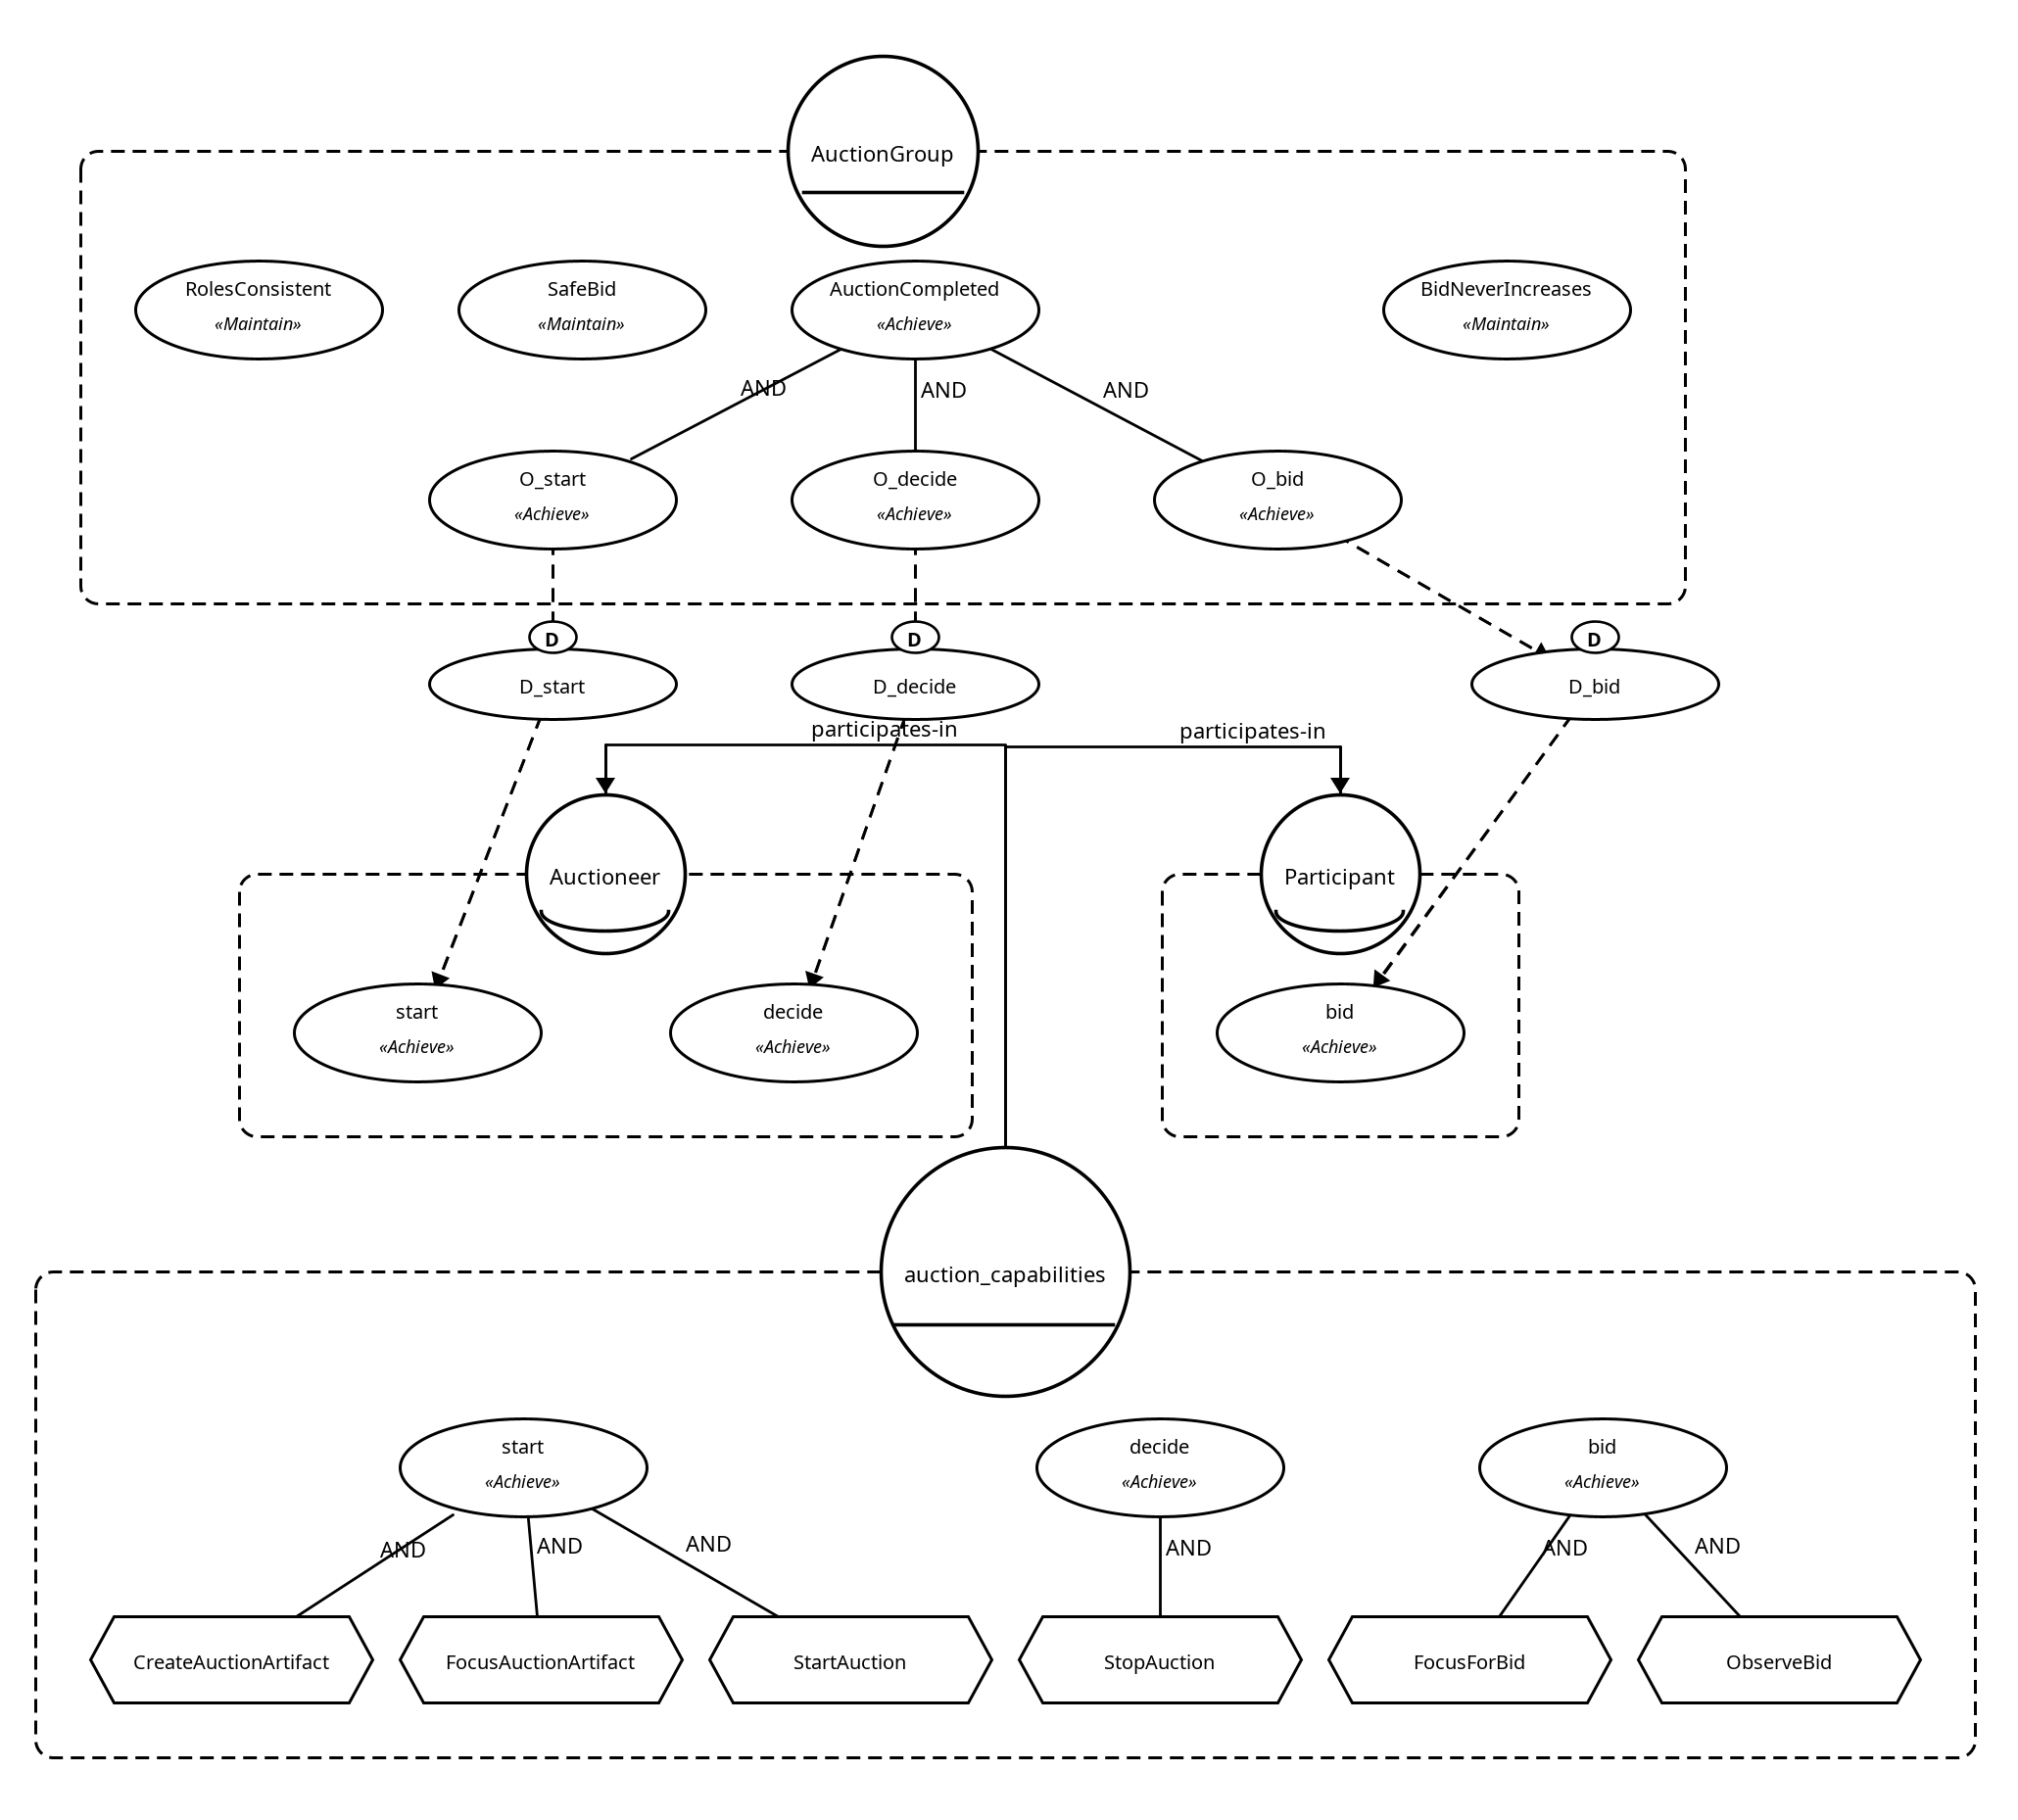
\includegraphics[width=6.09in,height=\textheight]{figures/fig-2-4.png}
\caption{Mô hình mục tiêu AuctionGroup.}\label{fig:2-4}
\end{figure}

Trong mô hình AuctionGroup ở \thesisfigure{fig:2-4}, mục tiêu AuctionCompleted có ba nhánh AND dành cho mở phiên, trả giá và quyết định kết quả. Goal SafeBid có kiểu Maintain và dùng điều kiện giá tốt nhất không âm. Bộ kiểm chứng theo dõi các điều kiện này riêng cho mỗi đối tượng Auction, như hai phiên được đối chiếu trong Mục 3.5.1. Trên biểu đồ của thẻ iStar Model, USE biểu diễn Goal bằng hình elip, Task bằng hình lục giác và ghi kiểu thời gian dưới tên Goal. Khi bật Show OCL contracts, các nhãn condition, pre và post phân biệt điều kiện của Goal với tiền và hậu điều kiện của Task. Đường tinh chỉnh ghi nhãn AND hoặc OR. Quan hệ phụ thuộc nối các chủ thể qua phần tử được phụ thuộc bằng nét đứt. Trong thẻ iStarSCN, người đọc chọn ngữ cảnh để xem trạng thái đánh giá trong phiên chạy. Kiểu thời gian thuộc đặc tả, còn trạng thái đánh giá được xác định qua quan sát.

\section{Ánh xạ trạng thái JaCaMo sang CSL}\label{sec:2-6}

Để chuyển dữ liệu JaCaMo về cấu trúc CSL đã mô tả ở Mục 2.4, người đặc tả khai báo nguồn và đích của từng luật trong XML. USE kiểm tra các luật trước khi khởi chạy. Tại mỗi checkpoint, bộ thu đồng bộ dữ liệu nguồn để bộ chiếu áp dụng các luật đó và dựng trạng thái đối tượng trong USE.

\subsection{Khai báo tương ứng bằng XML}\label{sec:2-6-1}

Mỗi luật xác định loại và kiểu của nguồn, trường cần đọc và thuộc tính đích. Nguồn có dạng category:sourceType/property:member đối với thuộc tính quan sát hoặc category:sourceType/identity:member đối với thông tin định danh. Loại nguồn gồm artifact, agent, organization, group. Trường định danh hỗ trợ name, uuid, workspace. Đích có dạng CslType.attribute.

Một luật chỉ áp dụng cho thể hiện có cả loại và kiểu nguồn khớp với khai báo. Giá trị đọc từ trường nguồn được chuyển sang kiểu USE của thuộc tính đích trước khi gán. AttributeMapping.read kiểm tra namespace và cấu trúc XML, đồng thời từ chối hai luật ghi cùng thuộc tính đích hoặc hai cặp loại và kiểu nguồn khác nhau cùng khai báo thể hiện cho một kiểu CSL. Khi khởi tạo, SnapshotProjection kiểm tra artifact tương ứng với Entity, còn tác tử, tổ chức và nhóm tương ứng với OrgContext. Thuộc tính đích phải tồn tại và có thể gán.

\begin{longtable}[]{@{}
  >{\raggedright\arraybackslash}p{(\columnwidth - 4\tabcolsep) * \real{0.2207}}
  >{\raggedright\arraybackslash}p{(\columnwidth - 4\tabcolsep) * \real{0.2276}}
  >{\raggedright\arraybackslash}p{(\columnwidth - 4\tabcolsep) * \real{0.5379}}@{}}
\caption{Luật ánh xạ thuộc tính của Auction}\label{tab:2-1}\tabularnewline
\toprule\noalign{}
\begin{minipage}[b]{\linewidth}\raggedright
\textbf{Loại và kiểu nguồn}
\end{minipage} & \begin{minipage}[b]{\linewidth}\raggedright
\textbf{Dữ liệu đọc}
\end{minipage} & \begin{minipage}[b]{\linewidth}\raggedright
\textbf{Thuộc tính đích trong CSL}
\end{minipage} \\
\midrule\noalign{}
\endfirsthead
\toprule\noalign{}
\begin{minipage}[b]{\linewidth}\raggedright
\textbf{Loại và kiểu nguồn}
\end{minipage} & \begin{minipage}[b]{\linewidth}\raggedright
\textbf{Dữ liệu đọc}
\end{minipage} & \begin{minipage}[b]{\linewidth}\raggedright
\textbf{Thuộc tính đích trong CSL}
\end{minipage} \\
\midrule\noalign{}
\endhead
\bottomrule\noalign{}
\endlastfoot
Tổ chức auction & Tên tổ chức & AuctionOrg.name \\
Nhóm auctionGroup & Tên nhóm & auctionGroup.name \\
Tác tử auction\_capabilities & Tên tác tử & auction\_capabilities.name \\
Artifact kiểu AuctionArtifact & Tên và bốn thuộc tính quan sát & Auction.id, Auction.running, Auction.task, Auction.best\_bid, Auction.winner \\
\end{longtable}

XML quy định cách lấy một giá trị từ nguồn và gán vào thuộc tính đích. Các liên kết như quan sát, thành viên và đảm nhiệm vai trò được dựng từ những quan hệ thực tế trong ảnh chụp. \thesistable{tab:2-1} liệt kê các luật gán thuộc tính dùng trong Auction.

\begin{samepage}

\thesisdisplaytitle{Đoạn mã 2.1}{Luật ánh xạ giá tốt nhất}

\begin{Verbatim}
<attribute source="artifact:auction_env.AuctionArtifact/property:best_bid"
target="Auction.best_bid"/>
\end{Verbatim}

\end{samepage}

Đoạn mã 2.1 đọc giá tốt nhất từ artifact và gán vào thuộc tính tương ứng của đối tượng Auction trong CSL. Cùng một luật có thể áp dụng cho nhiều artifact cùng lớp. Khi đó mỗi giá trị vẫn được gán cho đối tượng của chính artifact đã cung cấp giá trị. Quy tắc xác định đối tượng đích được trình bày ở Mục 2.6.3.

\subsection{Đồng bộ JaCaMo với CSL}\label{sec:2-6-2}

Bộ theo dõi chọn checkpoint dựa trên các sự kiện thực thi của Jason. Sau khi chọn ranh giới, bộ điều phối tạm giữ phần hoạt động thuộc phạm vi theo dõi để thu dữ liệu tại mốc đó. Trước khi các tác tử bắt đầu, JaCaMoCheckpoints.initial tạo checkpoint INITIAL. Khi một plan gốc thực thi, các plan con đồng bộ được theo dõi trong cùng nhóm. Monitor.finish tạo mốc PLAN\_COMPLETED khi nhóm kết thúc, gồm trường hợp hoàn thành, lỗi hoặc hủy được theo dõi. Một plan chạy trong intention độc lập tạo nhóm riêng. Khi một goal thất bại mà không có nhóm phù hợp đang xử lý sự kiện, bộ theo dõi có thể tạo GOAL\_FAILED. Nếu nguồn không còn quan sát được theo yêu cầu, nó tạo SOURCE\_UNAVAILABLE và đánh dấu ảnh chụp thiếu.

Khi gửi thông điệp cho tác tử khác, Monitor.send có thể giữ việc giao thông điệp tại AGENT\_HANDOFF. Nếu thông điệp không phải yêu cầu hỏi và chỉ còn các bước kết thúc nhóm, việc giao có thể dùng chung mốc PLAN\_COMPLETED. Mục 2.7.4 trình bày điều kiện để việc giao tiếp tục. Do chính sách chọn mốc dựa trên ranh giới thực thi, một thay đổi xuất hiện rồi biến mất bên trong nhóm plan có thể không có mặt trong các ảnh chụp.

JaCaMoCheckpoints.submit đưa yêu cầu vào hàng đợi và đóng tiếp nhận công việc mới bằng ExecutionBarrier.closeAdmission. Luồng điều phối đợi ExecutionBarrier.awaitFrozen xác nhận các hoạt động nguồn đã được cấp phép và các công việc chờ được theo dõi đã đạt trạng thái ổn định. StateProducer chỉ thu ảnh chụp khi có xác nhận đúng phiên, cổng tiếp nhận đã đóng, đồng hồ logic đã đóng băng và không còn hoạt động đang chạy hoặc công việc đang chờ trong phạm vi theo dõi. Các yêu cầu ở cùng đợt giữ có thể dùng chung một lần đóng băng nhưng mỗi checkpoint vẫn có token và số thứ tự riêng.

StateProducer.Connection.capture duyệt cây workspace cục bộ và thu các artifact đã khai báo trong ánh xạ, gồm định danh, lớp Java, thuộc tính quan sát và tác tử đang quan sát artifact. Hàm cũng lấy định danh tác tử, kiểu từ tên nguồn AgentSpeak, kiểu tổ chức và nhóm từ đặc tả Moise, cùng dữ kiện thành viên và đảm nhiệm vai trò từ trạng thái chạy. Giá trị thuộc tính đơn được giữ ở dạng số, chuỗi hoặc Boolean. Atom đơn và giá trị enum được chuyển thành tên tương ứng. Thông tin niềm tin, plan và intention dành cho màn hình quan sát và truy vết.

Mỗi yêu cầu mang mã lần chạy, số thứ tự ảnh, cờ complete, token và thông tin đợt giữ dừng. CheckpointProtocol.encodeSnapshot và decodeSnapshot chuyển đổi biểu diễn truyền nhận. Cờ complete cho biết lần thu có đầy đủ theo phạm vi quan sát hay không. Bước chiếu ở Mục 2.6.3 kiểm tra từng giá trị mà mô hình yêu cầu. \thesisfigure{fig:2-6} ở Mục 2.7.4 minh họa các mốc thu trạng thái và quyết định tương ứng.

\subsection{Chiếu đối tượng, thuộc tính và quan hệ}\label{sec:2-6-3}

Phép chiếu nhận ảnh chụp JaCaMo và dùng các luật đã khai báo ở Mục 2.6.1. SnapshotVerifier.update kiểm tra mã lần chạy và thứ tự ảnh trước khi chiếu dữ liệu. Nếu số thứ tự và nội dung trùng với ảnh vừa xử lý, USE có thể trả lại kết quả đã có. Khi complete=false, công cụ giữ nguyên trạng thái đối tượng và chuyển sang quyết định HOLD\_UNVERIFIED ở Mục 2.7.4.

Với một ảnh chụp đầy đủ, SnapshotProjection.prepare tạo tập hàng đối tượng và tập liên kết. indexSources lập chỉ mục theo định danh nguồn và từ chối định danh trùng. mapObjects chọn các luật theo loại và kiểu, rồi gọi decodeValue để chuyển giá trị theo kiểu USE đã khai báo. Số nguyên phải biểu diễn chính xác trong miền 32 bit, giá trị Real phải hữu hạn, còn giá trị enum phải khớp tên một hằng đã khai báo. Giá trị thiếu hoặc sai kiểu làm phép chiếu không thực hiện được. Với mã lần chạy r, định danh nguồn u và kiểu đích C, khóa của một đối tượng được xác định theo bộ sau.

\[K(r,u,C) = (r,u,C)\]

Vì vậy, nhiều thể hiện cùng kiểu vẫn tạo các đối tượng riêng. Việc quan sát lại cùng thể hiện giữ nguyên khóa và cho phép cập nhật đúng đối tượng. Đối với quan hệ, addFocusLinks đọc dữ kiện quan sát để dựng CslFocuses, addScopeLinks giải ngữ cảnh sở hữu theo vị trí nguồn và khai báo CSL, còn addMembershipLinks đọc quan hệ thành viên đã thu. addEnactments tạo thể hiện vai trò từ dữ kiện đảm nhiệm và nối với ngữ cảnh, chủ thể tương ứng qua InContext và Plays. Nếu một đầu liên kết cần thiết bị thiếu hoặc có nhiều cách xác định, phép chiếu báo lỗi.

Sau khi chuẩn bị hàng đối tượng và liên kết, SnapshotVerifier.applySnapshot tạo hoặc tìm đối tượng theo khóa, gán giá trị và dựng lại các liên kết từ dữ liệu đã chuẩn bị. Đối tượng vắng mặt trong ảnh đầy đủ được xóa cùng phiên theo dõi Goal và Task của đối tượng đó, nếu có. Bước này tạo trạng thái USE dùng ở Mục 2.7.

\begin{samepage}

\thesisdisplaytitle{Thuật toán 2.1}{Chiếu ảnh chụp sang trạng thái CSL}

\begin{Verbatim}[fontfamily=\rmdefault]
Đầu vào: snapshot s, mô hình CSL đã biên dịch, ánh xạ M,
trạng thái USE và lịch sử đánh giá của phiên
Đầu ra: trạng thái CSL mới và ảnh trạng thái trước,
hoặc chẩn đoán chưa đủ căn cứ kiểm chứng
1. Kiểm tra lần chạy, thứ tự và độ đầy đủ của s.
2. Lập chỉ mục dữ kiện nguồn theo định danh.
3. Với mỗi nguồn phù hợp M, giải kiểu đích và giải mã giá trị.
4. Tạo hàng đối tượng theo khóa K và xác định các liên kết.
5. Nếu không giải được giá trị hoặc đầu liên kết, trả chẩn đoán.
6. Lưu trạng thái USE trước. Tạo hoặc cập nhật các đối tượng.
7. Xóa liên kết cũ và các đối tượng vắng mặt trong snapshot đủ.
8. Dựng lại liên kết đã chuẩn bị. Trả cặp trạng thái trước và sau.
\end{Verbatim}

\end{samepage}

Có thể tách đường xử lý thành bước chuẩn bị phép chiếu và bước áp dụng vào USE. Trong bước đầu, SnapshotProjection.prepare xác định kiểu đích, chuyển đổi giá trị và giải các đầu liên kết trên biểu diễn trung gian. Chỉ sau khi các kiểm tra đó thành công, SnapshotVerifier.update mới lưu trạng thái trước và gọi applySnapshot. Thuật toán 2.1 tóm tắt các bước quan trọng theo thứ tự thực hiện.

Sự vắng mặt của một đối tượng chỉ có ý nghĩa khi snapshot đầy đủ. Ví dụ, một chế độ quan sát bị gián đoạn có thể trả danh sách rỗng, nhưng điều đó chưa chứng minh đối tượng đã biến mất. Vì vậy bước kiểm tra độ đầy đủ chạy trước khi chiếu. Với snapshot đầy đủ đến được bước áp dụng, lịch sử của đối tượng bị xóa cũng được kết thúc. Việc kiểm tra trước khi áp dụng chặn các lỗi dữ liệu được phát hiện trong bước chuẩn bị. Nếu lỗi xảy ra trong lúc áp dụng trực tiếp vào MSystem, mã hiện hành có thể đã thay đổi một phần trạng thái trước khi trả giữ dừng.

\begin{figure}
\centering
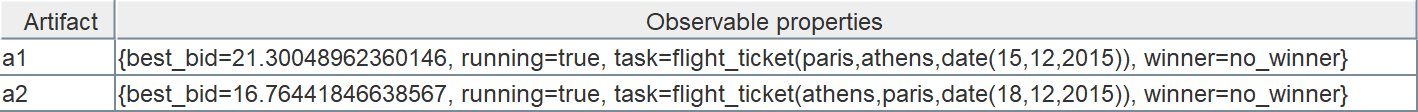
\includegraphics[width=6.1in,height=\textheight]{figures/fig-2-5.png}
\caption{Trạng thái Auction trong JaCaMo và USE.}\label{fig:2-5}
\end{figure}

\thesisfigure{fig:2-5} ghi lại checkpoint 45 của phiên Auction 3ca479bf. Thẻ Artifacts hiển thị giá 12,25180855001036 cho a1 và 61,79266359141802 cho a2. Hai đối tượng CSL trong OAL State giữ đúng các giá trị tương ứng.

\section{Kiểm chứng ràng buộc và đánh giá Goal/Task}\label{sec:2-7}

Sau khi chiếu dữ liệu, USE dùng trạng thái mới để kiểm tra bất biến và dùng cặp trạng thái trước và sau lần cập nhật, cùng lịch sử của từng ngữ cảnh, để đánh giá Goal và Task. Kết quả của các phép đánh giá được chuyển sang bước tổng hợp quyết định tại checkpoint (Mục 2.7.4).

\subsection{Đánh giá OCL trên trạng thái CSL}\label{sec:2-7-1}

Gọi \(\sigma_{k}\) là trạng thái CSL sau khi áp dụng snapshot tại checkpoint k và \(\sigma_{k-1}\) là trạng thái ngay trước lần cập nhật đó. Trong SnapshotVerifier.update, công cụ lưu lại trạng thái USE trước khi gọi applySnapshot, rồi dùng StateView.pin để cố định cặp trạng thái trong khi đánh giá. NativeOclBackend.compile kiểm tra và biên dịch trước biểu thức theo kiểu ngữ cảnh của self. Khi đánh giá một biểu thức \(\varphi\) trên đối tượng o, NativeOclBackend.evaluate truyền cặp trạng thái và gán self cho o trong bộ đánh giá OCL của USE~\cite{ref-4}.

\[v_{k}(\varphi,o) = {eval}_{OCL}\left( \varphi,\sigma_{k - 1},\sigma_{k},\{ self \mapsto o\} \right).\]

Các tham chiếu thông thường đọc \(\sigma_{k}\). Trong những điều kiện cho phép dùng @pre, ký hiệu này đọc \(\sigma_{k-1}\). Vì vậy, so sánh qua @pre chỉ phản ánh cặp trạng thái mà bộ kiểm chứng quan sát được. Với bất biến \(\varphi\) khai báo trên kiểu C, checkInvariants áp dụng biểu thức cho từng đối tượng thuộc C hoặc lớp con của C.

\[\sigma_{k} \vDash \varphi\quad \Leftrightarrow \quad\forall o \in {Inst}_{\sigma_{k}}(C):v_{k}(\varphi,o) = true.\]

Bộ đánh giá trả PASS khi biểu thức đúng và FAIL khi biểu thức sai. Giá trị không xác định, lỗi và phép kiểm tra bị bỏ qua có mã riêng UNDEFINED, ERROR và SKIPPED. Một điều kiện của Goal hoặc Task nhận FAIL mới chỉ cung cấp giá trị sai cho quy tắc đánh giá tương ứng. Khi phép kiểm tra của một ngữ cảnh cho kết quả ngoài PASS và FAIL, checkGoalTasks bỏ qua cập nhật lịch sử của ngữ cảnh đó.

\begin{samepage}

\thesisdisplaytitle{Đoạn mã 2.2}{Bất biến của Auction}

\begin{Verbatim}
context Auction inv ValidBid:
self.best_bid >= 0;
context Auction inv RunningAuctionIsObserved:
self.running implies self.focusedBy->exists(a |
self.cslEntityScope.oclAsType(auctionGroup).auctioneer->exists(r | r.player = a));
\end{Verbatim}

\end{samepage}

ValidBid kiểm tra giá tốt nhất của đối tượng đang xét. RunningAuctionIsObserved yêu cầu khi đấu giá đang mở phải có ít nhất một tác tử quan sát artifact và đảm nhiệm vai trò auctioneer trong nhóm tương ứng.

\subsection{Đánh giá Task theo lịch sử tiền và hậu điều kiện}\label{sec:2-7-2}

Bảng I của \cite{ref-28} xác định giá trị tức thời của Task từ tiền và hậu điều kiện. Phiên bản kiểm chứng JaCaMo dùng TaskMarking.update để tích lũy bằng chứng qua các checkpoint. Với một Task trong một ngữ cảnh, gọi \(p_{k}\) và \(r_{k}\) là giá trị Boolean của tiền điều kiện và hậu điều kiện tại checkpoint k. Hai cờ \(Q_{k}\) và \(R_{k}\) ghi nhớ đã thấy tiền điều kiện và đã thấy hậu điều kiện ở hoặc sau mốc thỏa tiền điều kiện. Khởi đầu \(Q_{0}\) = \(R_{0}\) = 0. Khi Task được yêu cầu và cả hai giá trị đều xác định, công cụ cập nhật.

\[Q_{k} = Q_{k - 1} \vee p_{k},\quad\quad R_{k} = R_{k - 1} \vee \left( Q_{k} \land r_{k} \right).\]

Task ở trạng thái UNKNOWN nếu \(Q_{k}\) = 0, PENDING nếu \(Q_{k}\) = 1 và \(R_{k}\) = 0, và FULFILLED nếu \(R_{k}\) = 1. Việc dùng \(Q_{k}\) ở vế phải cho phép ghi nhận cả hai điều kiện ngay tại một checkpoint. GoalTaskSession.step lưu cặp cờ riêng cho từng thể hiện Task trong ngữ cảnh của đối tượng.

\begin{samepage}

\thesisdisplaytitle{Đoạn mã 2.3}{Điều kiện của StopAuction}

\begin{Verbatim}
task StopAuction > decide
pre {[ self.running ]}
post {[ not self.running ]}
\end{Verbatim}

\end{samepage}

Trạng thái running = false có thể chỉ một phiên chưa mở hoặc một phiên đã đóng. Bộ kiểm chứng ghi nhận StopAuction hoàn thành khi đã quan sát phiên mở và sau đó thấy chính phiên ấy đóng.

\subsection{Đánh giá Goal và lan truyền kết quả}\label{sec:2-7-3}

Đối với Goal có điều kiện OCL trực tiếp, GoalMarking.update dùng bộ ba (\(A_{k}\), \(P_{k}\), \(S_{k}\)). \(A_{k}\) cho biết Goal đang hoạt động, \(P_{k}\) ghi nhận giá trị điều kiện theo loại Goal và \(S_{k}\) ghi nhận điều kiện có giữ được sau khi đã đúng hay không. Gọi \(b_{k}\) là kết quả OCL đã xác định. Với Achieve, \(P_{k}\) = \(P_{k-1}\) \(\lor\) \(b_{k}\). Với Maintain, Sustain và None, \(P_{k}\) = \(b_{k}\). Cờ ổn định được tính theo quy tắc~\cite{ref-28}.

\[S_{k} = S_{k - 1} \land \left( \neg P_{k - 1} \vee P_{k} \right).\]

Khi bắt đầu đánh giá, lấy \(S_{k-1}\) = 1 và lấy \(P_{k-1}\) = 1 riêng cho Maintain, bằng 0 cho các loại khác. Achieve giữ kết quả đạt sau lần quan sát đúng đầu tiên. None theo giá trị tại mốc hiện tại. Maintain chỉ đạt khi \(P_{k}\) và \(S_{k}\) đều đúng, nên điều kiện sai ở lần đầu đã cho kết quả vi phạm. Sustain cho phép trạng thái chờ trước lần đúng đầu tiên nhưng báo vi phạm nếu mất điều kiện sau đó. Goal chưa hoạt động mang trạng thái UNKNOWN. Trong đường kiểm chứng này, SnapshotVerifier.goalTaskInputs cung cấp cờ hoạt động cho những Goal có điều kiện trực tiếp ở ngữ cảnh đang xét.

Với các phần tử suy ra từ quan hệ trong mô hình, GoalTaskSession.step dựng kết quả tổng hợp từ lịch sử đã cập nhật. Công cụ gọi IStarMarking.closePending và assignGoalTask cho các phân rã, gọi GoalModelInstanceTranslator.propagateDependencies cho các phụ thuộc, rồi tính lại kết quả phân rã. Với AND, một nhánh vi phạm làm kết quả vi phạm, còn kết quả đạt cần tất cả nhánh đạt. Với OR, một nhánh đạt đủ để cho kết quả đạt. Khi chưa có nhánh đạt, một nhánh đang chờ cho kết quả chờ. Nếu chỉ có nhánh vi phạm hoặc chưa xác định và có ít nhất một nhánh vi phạm, mã hiện tại trả VIOLATED. Bảng I của \cite{ref-28} có quy tắc truyền cả kết quả đạt và vi phạm qua quan hệ phụ thuộc. Trong mã hiện tại, hàm lan truyền phụ thuộc chỉ truyền FULFILLED từ phần tử được trông cậy sang phần tử phụ thuộc.

\begin{samepage}

\thesisdisplaytitle{Đoạn mã 2.4}{Điều kiện của BidNeverIncreases}

\begin{Verbatim}
goal BidNeverIncreases : Maintain condition {[
Auction.allInstances@pre()->excludes(self) or self.best_bid <= self.best_bid@pre
]}
\end{Verbatim}

\end{samepage}

Nếu đối tượng đã tồn tại, giá tốt nhất hiện tại phải nhỏ hơn hoặc bằng giá tại mốc trước. Khi USE quan sát thấy giá tăng, kiểu Maintain ghi nhận mục tiêu bị vi phạm.

\subsection{Tổng hợp quyết định checkpoint}\label{sec:2-7-4}

Sau khi kiểm tra bất biến và đánh giá Goal, Task, USE tổng hợp kết quả để quyết định cho JaCaMo tiếp tục hay giữ dừng tại chính checkpoint đang chờ. Gọi \(I_{k}\) là tập các lần đánh giá bất biến CSL tại checkpoint thứ k, \(C_{k}\) là tập kết quả kiểm tra gồm bất biến và điều kiện iStar, còn \(E_{k}\) là tập kết quả Goal/Task được tạo tại mốc đó. Từ các tập này, SnapshotVerifier.update xác định \(F_{k}\) để ghi nhận vi phạm đã xác định và \(U_{k}\) để ghi nhận phép kiểm tra chưa cho kết quả đúng hoặc sai.

\[F_{k} = \left( \exists i \in I_{k}:verdict(i) = FAIL \right) \vee \left( \exists e \in E_{k}:status(e) = VIOLATED \right).\]

\[U_{k} = \exists c \in C_{k}:verdict(c) \notin \{ PASS,FAIL\}.\]

\[D_{k} = \left\{ \begin{matrix}
HOLD\_ FAILURE, & F_{k} \\
HOLD\_ UNVERIFIED, & \neg F_{k} \land U_{k} \\
APPROVE, & \neg F_{k} \land \neg U_{k}.
\end{matrix} \right.\ \]

Công thức trên áp dụng khi ảnh chụp đầy đủ và đi qua đường đánh giá. Khi ảnh chụp được đánh dấu thiếu, SnapshotVerifier.update trả HOLD\_UNVERIFIED trước bước chiếu. Nếu quá trình xử lý ảnh chụp phát sinh ngoại lệ, VerificationSession.handleCheckpoint tạo phản hồi HOLD\_UNVERIFIED thay cho kết quả đánh giá. Trong đường đánh giá thông thường, một vi phạm đã xác định được ưu tiên hơn kết quả chưa xác định ở phép kiểm tra khác. Một tiền hoặc hậu điều kiện cho kết quả FAIL có thể chỉ phản ánh tiến độ chưa đạt. Trạng thái PENDING của Task hay kết quả FAILED của plan ở metadata nguồn cũng không tự chúng được tính là vi phạm.

Khi nhận quyết định từ USE, StateProducer xác thực phản hồi và dùng CheckpointProtocol.approved để đối chiếu phiên, token, mã băm yêu cầu, phạm vi giữ dừng và kết quả. JaCaMoCheckpoints.drain chỉ mở lại cổng tiếp nhận sau khi tất cả yêu cầu trong đợt giữ được phê duyệt và hàng đợi đã hết. Nếu có HOLD, hết thời gian chờ hoặc lỗi truyền, phía nguồn không mở cổng. Với mốc INITIAL, thiếu phê duyệt ngăn bước khởi chạy tác tử. Quyết định APPROVE vì vậy có hiệu lực đối với điểm giữ dừng đã được kiểm tra trong phạm vi quan sát.

\begin{figure}
\centering
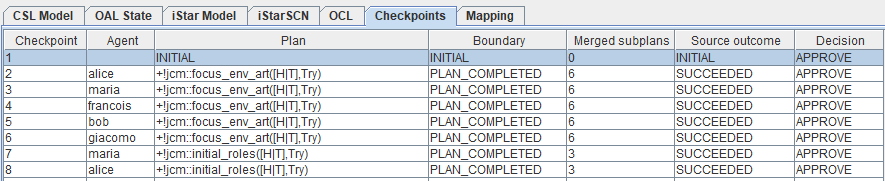
\includegraphics[width=6.09in,height=\textheight]{figures/fig-2-6.png}
\caption{Các checkpoint của Auction.}\label{fig:2-6}
\end{figure}

\thesisfigure{fig:2-6} cho thấy checkpoint khởi tạo và các mốc kết thúc nhóm plan trong một lần chạy Auction. Cột Decision ghi APPROVE ở các mốc được hiển thị. Trong ca ở Mục 2.2.1, JaCaMo cũng được phép tiếp tục dù a1 còn chờ một lượt trả giá tốt hơn. Trạng thái PENDING khi đó phản ánh tiến độ của nhiệm vụ. Nếu USE xác định một Goal đã bị vi phạm, nó trả HOLD\_FAILURE ngay cả khi các bất biến đều đạt. Ảnh chụp, kết quả đánh giá và phản hồi được lưu tại từng checkpoint, làm cơ sở đối chiếu kết quả khi đánh giá lại cùng vết với cùng đặc tả (Mục 3.5.3).

\section{Tổng kết chương}\label{sec:2-8}

Phương pháp gồm bốn bước. Đặc tả CSL xác định cấu trúc trạng thái, còn iStar mở rộng xác định các mục tiêu, nhiệm vụ và điều kiện cần theo dõi. Phép ánh xạ đưa dữ liệu JaCaMo tại checkpoint vào cấu trúc đã khai báo. Trên trạng thái đó, USE kiểm tra bất biến, đánh giá Goal và Task, rồi tổng hợp quyết định cho phép tiếp tục hoặc giữ dừng tại đúng checkpoint.

Phép ánh xạ bảo toàn định danh để mỗi đối tượng có lịch sử riêng. Quyết định giữ dừng phân biệt vi phạm đã xác định với trường hợp chưa đủ dữ liệu. Phạm vi kết luận phụ thuộc vào các ranh giới quan sát và điều kiện đã đặc tả. Chương 3 đối chiếu từng cơ chế qua thực nghiệm Auction, Counter và đánh giá lại vết.

\chapter{TRIỂN KHAI VÀ THỰC NGHIỆM}\label{sec:3}

Công cụ được triển khai dưới dạng plugin USE. Một tiến trình JaCaMo cung cấp dữ liệu thực thi cho bộ kiểm chứng tại từng checkpoint. Chương này trình bày cách tổ chức công cụ và các ca dùng để đối chiếu phương pháp với kết quả thực thi.

\section{Giới thiệu}\label{sec:3-1}

Thực nghiệm xem xét cách phương pháp ở Chương 2 hoạt động khi nhiều đối tượng cùng kiểu được kiểm chứng trong một phiên chạy. Việc giữ định danh và lịch sử riêng cho từng đối tượng cho phép đối chiếu quyết định tại một checkpoint với bằng chứng của chính đối tượng đó. Đánh giá lại cùng vết với cùng cấu hình còn cho phép kiểm tra liệu các quyết định và trạng thái Goal, Task có được tái hiện tại từng mốc hay không.

TN01 theo dõi hai cuộc đấu giá trong USE, còn TN02 đánh giá lại chính vết đã ghi. TN03 và TN04 lần lượt tạo một vi phạm bất biến và một ảnh chụp được báo là thiếu dữ liệu. TN05--TN07 bổ sung các tình huống vi phạm Goal, thiếu một thuộc tính bắt buộc và sai lệch xuất hiện giữa hai mốc quan sát. Ba ca bổ sung thu vết qua dòng lệnh, còn các lần chụp giao diện dùng cấu hình tương ứng để minh họa kết quả.

Các ca thử được thực hiện trên công cụ mô tả ở Mục 3.2, theo cấu hình và tiêu chí đánh giá trình bày tại Mục 3.3--3.4. Mục 3.5 phân tích bằng chứng thu được từ các lần chạy, qua đó xác định phạm vi kết luận và các hướng mở rộng trong Mục 3.6.

\section{Triển khai công cụ}\label{sec:3-2}

Công cụ kết nối JaCaMo với USE qua cơ chế checkpoint. Cách tổ chức plugin quyết định nơi lưu trạng thái kiểm chứng, còn cấu hình đầu vào xác định dữ liệu nào được sử dụng trong mỗi phiên.

\subsection{Tổ chức các thành phần}\label{sec:3-2-1}

Công cụ được đóng gói thành bản USE có thể chạy được qua module Maven use-assembly. Trong tiến trình USE, giao diện do use-gui cung cấp nạp plugin từ use-plugin và làm việc với mô hình, trạng thái đối tượng và bộ đánh giá OCL của use-core. Mỗi phiên có một MSystem riêng trong tiến trình chính để giữ mô hình và kết quả kiểm chứng. Trong khi đó, JaCaMo chạy trong JVM con để nạp runtime và mã Java của các artifact. Plugin xử lý ảnh chụp từ tiến trình con và trả quyết định về nguồn. Cách tổ chức này cho phép giao diện USE tiếp tục hiển thị kết quả khi JaCaMo đang chờ phản hồi tại checkpoint.

VerificationSession kiểm tra các tệp cấu hình và khởi chạy JaCaMo. Công cụ kiểm tra ảnh chụp khởi tạo trước khi cho các tác tử chạy. Ở các mốc sau, bộ thu chờ phần thực thi thuộc phạm vi theo dõi đi đến điểm ổn định rồi gửi ảnh chụp. SnapshotVerifier dựng trạng thái CSL, kiểm tra bất biến và đưa kết quả điều kiện vào bộ đánh giá Goal/Task. USE lưu kết quả và phản hồi tại đúng checkpoint. JaCaMo xác nhận phản hồi trước khi tiếp tục nếu được phê duyệt.

\subsection{Môi trường và cách khởi chạy}\label{sec:3-2-2}

TN01 và TN03 chạy trên Windows 11 với JDK 21, USE 7.5.0 và plugin 1.0.1. Ba ca TN05--TN07 chạy qua dòng lệnh trên Debian với cùng phiên bản mã USE và runtime kiểm chứng.

\begin{figure}
\centering
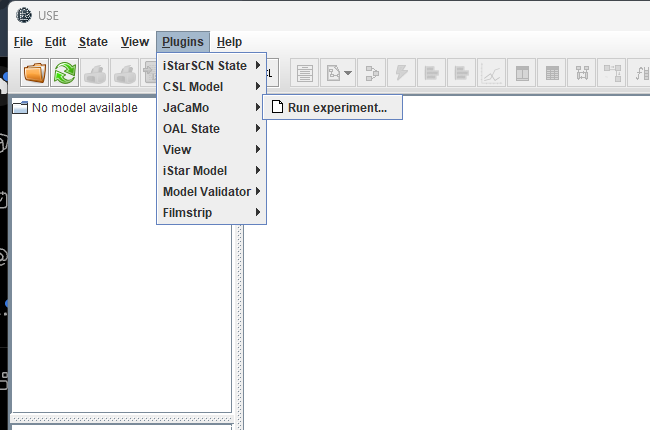
\includegraphics[width=3.95in,height=\textheight]{figures/fig-3-1.png}
\caption{Trình đơn thực nghiệm JaCaMo.}\label{fig:3-1}
\end{figure}

\thesisfigure{fig:3-1} cho thấy lệnh chạy thực nghiệm trong trình đơn Plugins của USE. Sau khi chọn JaCaMo và Run experiment, người dùng cung cấp các tệp mô tả phiên chạy.

\begin{figure}
\centering
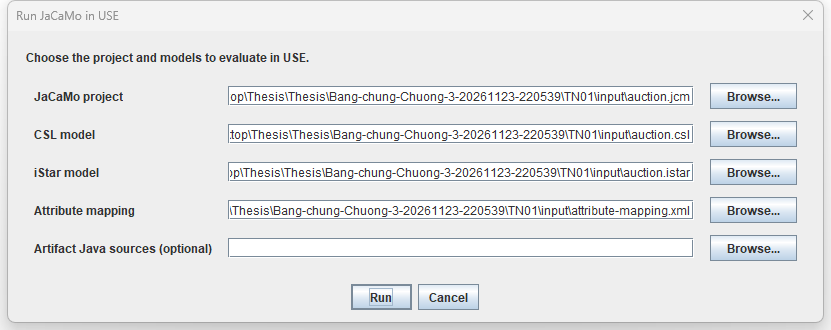
\includegraphics[width=6.03in,height=\textheight]{figures/fig-3-2.png}
\caption{Cấu hình đầu vào của TN01.}\label{fig:3-2}
\end{figure}

\thesisfigure{fig:3-2} trình bày bốn tệp đầu vào của TN01 gồm dự án JaCaMo (.jcm), đặc tả CSL, mô hình iStar và luật XML ánh xạ. Khi ô Artifact Java sources để trống, công cụ tìm mã Java trong thư mục src/env cạnh tệp .jcm. Sau khi khởi chạy, cửa sổ thực nghiệm hiển thị dữ liệu JaCaMo ở bên trái và kết quả kiểm chứng của USE ở bên phải. Người dùng chọn một hàng ở Checkpoints để đối chiếu dữ liệu nguồn, đối tượng CSL và kết quả iStar tại cùng một mốc.

Vết của USE ghi dữ liệu gửi đến và kết quả kiểm chứng. Sau khi nhận và xác nhận phản hồi, JaCaMo ghi một bản xác nhận cho checkpoint tương ứng. Log của chương trình nguồn giúp đối chiếu các thao tác phát sinh giữa hai lần chụp.

\section{Kịch bản thử nghiệm}\label{sec:3-3}

Các ca thử bắt đầu bằng việc chạy Auction và đánh giá lại dữ liệu đã thu. Các biến thể sau đó tạo vi phạm hoặc giới hạn dữ liệu quan sát để kiểm tra cách công cụ phản hồi tại từng checkpoint.

\subsection{Chạy Auction và đánh giá lại vết}\label{sec:3-3-1}

\begin{figure}
\centering
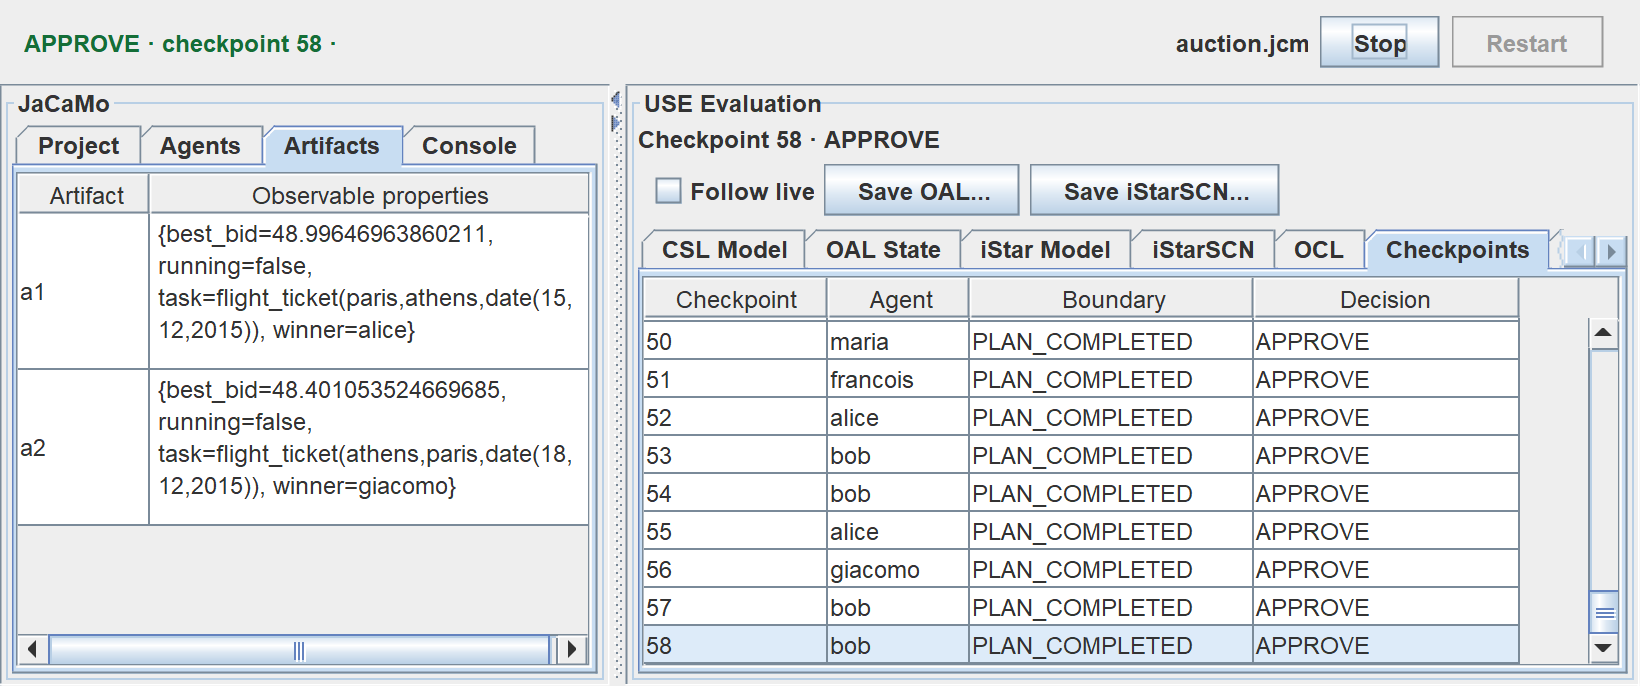
\includegraphics[width=6.1in,height=\textheight]{figures/fig-3-3.png}
\caption{Giao diện theo dõi Auction.}\label{fig:3-3}
\end{figure}

TN01 chạy Auction với hai phiên a1 và a2 dùng chung cấu trúc, điều kiện mục tiêu và luật ánh xạ. Ca thử kiểm tra liệu từng phiên có giữ được giá và tiến độ riêng qua các checkpoint hay không. \thesisfigure{fig:3-3} minh họa cửa sổ theo dõi tại checkpoint 58. Để kiểm tra khả năng tái hiện trên chính dữ liệu đó, TN02 dùng lại chuỗi snapshot và các tệp đặc tả của TN01. Bộ đánh giá xử lý lần lượt các ảnh đã ghi để so sánh quyết định và các phần tử đạt tại từng checkpoint.

\subsection{Vi phạm ràng buộc và thiếu dữ liệu}\label{sec:3-3-2}

TN03 dùng Counter với bất biến Nonnegative, yêu cầu giá trị bộ đếm không âm. Chương trình đặt giá trị thành −1 trước khi nhóm plan kết thúc. Tại mốc cuối, USE được kỳ vọng nhận biết vi phạm và giữ dừng. TN04 bổ sung tình huống mà ảnh chụp được báo là chưa đầy đủ nên công cụ chưa có đủ căn cứ để kiểm chứng. Bộ kiểm chứng nhận trước một đối tượng hợp lệ rồi nhận ảnh thiếu dữ liệu. Ca thử xác nhận đối tượng cũ vẫn còn và kết quả là HOLD\_UNVERIFIED. Khi thay ảnh thiếu bằng ảnh đầy đủ ở cùng mốc, công cụ được kỳ vọng phê duyệt.

\subsection{Ca đối chứng và giới hạn quan sát}\label{sec:3-3-3}

TN05 so sánh hai cách xử lý lượt trả giá kém hơn. Bản đối chứng giữ giá tốt nhất ở 10 khi nhận giá 20. Bản có lỗi thay giá tốt nhất bằng 20. Cả hai cách được thử khi các lượt trả giá nằm trong một nhóm plan và khi có thêm checkpoint chuyển giao giữa các lần cập nhật. Giá 20 vẫn thỏa bất biến yêu cầu giá không âm. Khi vết ghi cả giá 10 và 20 của cùng đối tượng, Goal BidNeverIncreases phải phát hiện bước tăng. So sánh hai cấu hình giúp xác định ảnh hưởng của ranh giới quan sát.

Hai ca còn lại khảo sát những giới hạn khác nhau của dữ liệu quan sát. Trong TN06, thuộc tính best\_bid bị bỏ khỏi bản sao của chương trình đấu giá, trong khi luật ánh xạ vẫn yêu cầu thuộc tính đó. Tình huống này cho phép kiểm tra cách công cụ phản hồi khi đã quan sát được đối tượng nguồn nhưng thiếu giá trị để dựng trạng thái CSL. TN07 xét giới hạn của thời điểm quan sát. Cả hai bản Counter đều đặt bộ đếm thành −1 như được ghi trong log nguồn. Một bản giữ giá trị đến cuối nhóm plan, còn bản kia đưa bộ đếm trở lại 2 trước khi nhóm kết thúc.

\section{Tiêu chí đánh giá}\label{sec:3-4}

Việc đánh giá bắt đầu bằng đối chiếu mỗi artifact JaCaMo với đối tượng CSL và lịch sử Goal, Task tương ứng. Tên, định danh và giá trị được so sánh tại cùng checkpoint rồi theo dõi qua nhiều mốc để phát hiện trường hợp dữ liệu của hai phiên bị trộn. Sau khi xác nhận sự kiện trong log nguồn và dữ liệu quan sát được trong snapshot, kết quả bất biến hoặc Goal được đối chiếu với quyết định của USE và bản xác nhận của JaCaMo. Qua đó có thể phân biệt quyết định giữ dừng vì có vi phạm với trường hợp thiếu căn cứ kiểm chứng. Khả năng tái hiện được đánh giá bằng cách xử lý lại cùng vết và cùng đặc tả, rồi so sánh quyết định và tập Goal, Task đã đạt ở mỗi checkpoint theo đúng đối tượng và chủ thể.

\section{Kết quả và phân tích}\label{sec:3-5}

Các kết quả được phân tích từ dữ liệu quan sát của từng đối tượng đến quyết định mà công cụ trả tại checkpoint. Việc đánh giá lại cùng vết cho biết các kết quả đó có được tái hiện khi dữ liệu đầu vào được giữ nguyên hay không.

\subsection{Định danh và lịch sử của từng đối tượng}\label{sec:3-5-1}

Trong TN01, hai artifact được ánh xạ thành hai đối tượng Auction tách biệt. USE giữ ổn định định danh đích qua các lần cập nhật. Ở checkpoint 39, cả hai phiên còn chờ lượt trả giá cải thiện. Đến checkpoint 42, a2 đã có mức giá tốt hơn trong khi a1 vẫn chờ. Kết quả cho thấy cùng một nhiệm vụ được theo dõi riêng cho từng phiên.

\begin{figure}
\centering
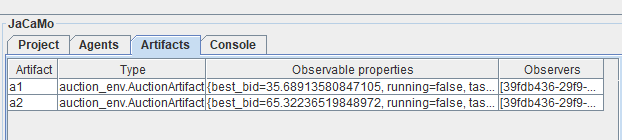
\includegraphics[width=5.9500in]{figures/fig-3-4-a.png}
\par\smallskip
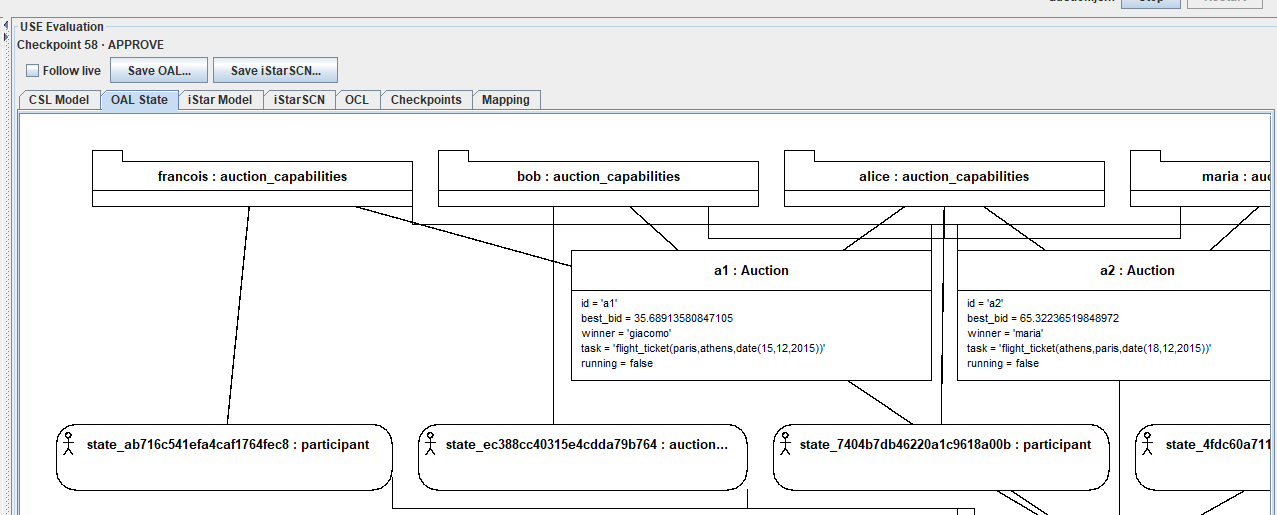
\includegraphics[width=6.1000in]{figures/fig-3-4-b.png}
\caption{Giá của hai phiên Auction trong USE.}\label{fig:3-4}
\end{figure}

Tại checkpoint 58, \thesisfigure{fig:3-4} đối chiếu giá trong Artifacts và OAL State. Giá của mỗi artifact xuất hiện đúng trên đối tượng CSL tương ứng.

\begin{figure}
\centering
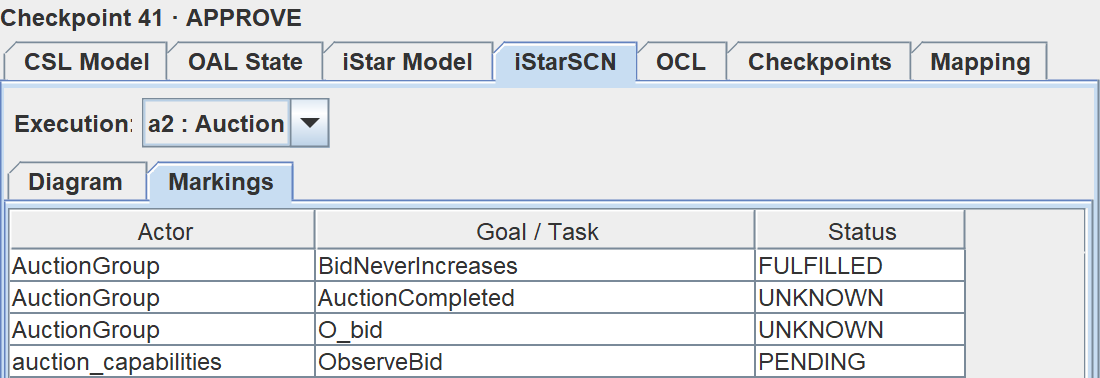
\includegraphics[width=6.1in,height=\textheight]{figures/fig-3-5.png}
\caption{Kết quả AuctionCompleted của phiên a1.}\label{fig:3-5}
\end{figure}

Ở cùng checkpoint, mục tiêu AuctionCompleted của phiên a1 đã đạt, như thể hiện trong \thesisfigure{fig:3-5}. Mục tiêu của phiên a2 được đánh giá trên ngữ cảnh riêng.

\begin{figure}
\centering
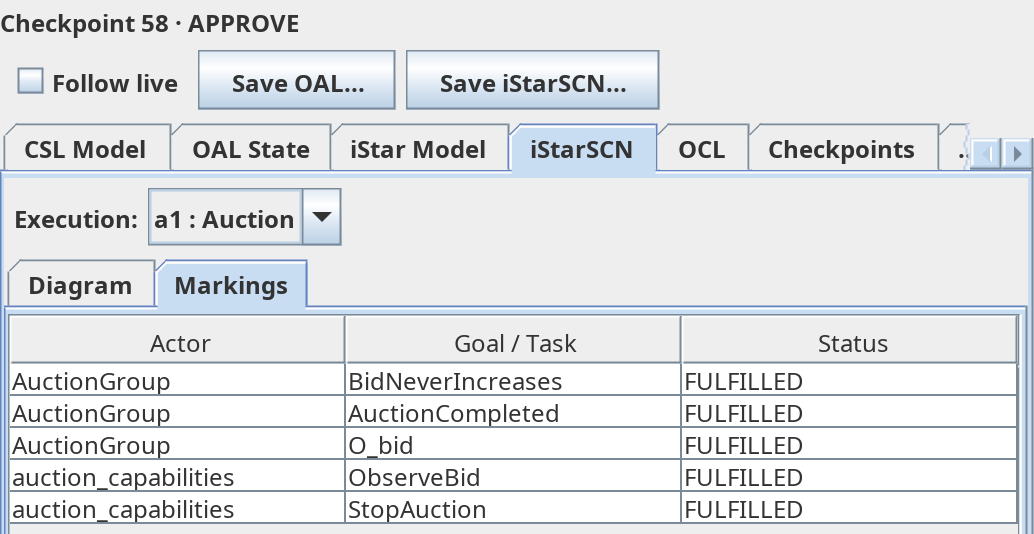
\includegraphics[width=6.1in,height=\textheight]{figures/fig-3-6.png}
\caption{Kết quả AuctionCompleted của phiên a2.}\label{fig:3-6}
\end{figure}

\thesisfigure{fig:3-6} ghi nhận AuctionCompleted cũng đã đạt ở phiên a2. Trong TN01, JaCaMo xác nhận đủ cả 58 quyết định APPROVE.

\subsection{Quyết định kiểm chứng và giới hạn quan sát}\label{sec:3-5-2}

Câu hỏi thứ hai xét đồng thời nguyên nhân quyết định và bằng chứng quyết định được chuyển về nguồn. TN03 kiểm tra một vi phạm còn quan sát được ở cuối nhóm plan. TN04 kiểm tra trường hợp ảnh chụp chưa đầy đủ và việc giữ đối tượng đã biết. Các ca bổ sung tiếp tục tách vi phạm Goal, thiếu thuộc tính và sự kiện chỉ xảy ra giữa hai lần chụp.

\begin{figure}
\centering
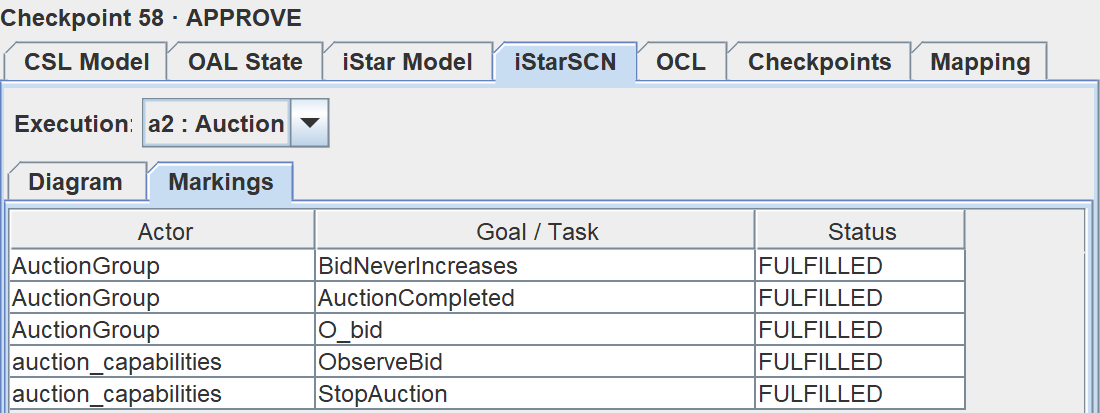
\includegraphics[width=6.1in,height=\textheight]{figures/fig-3-7.png}
\caption{Vi phạm bất biến của Counter.}\label{fig:3-7}
\end{figure}

Trong TN03 ở \thesisfigure{fig:3-7}, hai mốc đầu cho thấy bộ đếm bằng 0 và bất biến được thỏa. Tại mốc 3, nhóm plan kết thúc bình thường, nhưng trạng thái quan sát có giá trị −1. USE phát hiện vi phạm Nonnegative và trả HOLD\_FAILURE. Goal SafeValue cũng bị vi phạm tại mốc này, nên TN05 được dùng để xem xét riêng tác động của một Goal.

TN04 trả HOLD\_UNVERIFIED khi nhận ảnh chụp thiếu và vẫn giữ một đối tượng đã quan sát. Bộ kiểm chứng phê duyệt sau khi nhận ảnh đầy đủ thay thế tại cùng mốc.

TN05 xét vi phạm mục tiêu BidNeverIncreases. Khi hai lượt trả giá nằm trong cùng nhóm plan, log cho thấy giá tăng từ 10 lên 20 và snapshot chỉ ghi giá cuối. USE phê duyệt cả 27 checkpoint. Bản đối chứng giữ giá 10 sau lượt trả giá 20 và được phê duyệt ở cả 28 checkpoint.

\begin{figure}
\centering
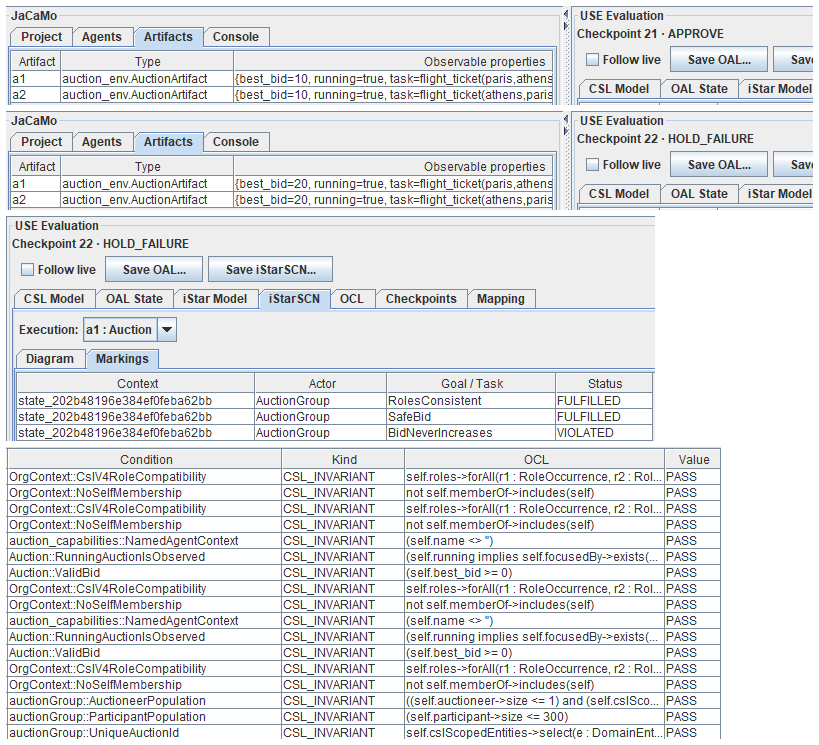
\includegraphics[width=6.1in,height=\textheight]{figures/fig-3-8.png}
\caption{Vi phạm BidNeverIncreases trong TN05.}\label{fig:3-8}
\end{figure}

Khi có thêm mốc chuyển giao, USE quan sát được giá 10 ở checkpoint 21 và 20 ở checkpoint 22. Mục tiêu BidNeverIncreases bị vi phạm, JaCaMo nhận HOLD\_FAILURE và log không ghi hoạt động sau điểm dừng. Phiên đối chứng dùng cùng ranh giới và tiếp tục ở cả 31 checkpoint. \thesisfigure{fig:3-8} ghi lại kết quả của phiên chụp 8ae8adb8. Tại checkpoint 22, cả 17 lượt đánh giá bất biến đều PASS, còn mục tiêu BidNeverIncreases có trạng thái VIOLATED.

\begin{figure}
\centering
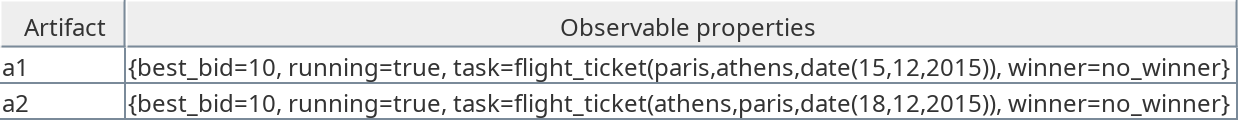
\includegraphics[width=6.1in,height=\textheight]{figures/fig-3-9.png}
\caption{Thiếu giá tốt nhất trong TN06.}\label{fig:3-9}
\end{figure}

Trong TN06, cả hai phiên đều thu được đối tượng Auction nhưng thiếu giá tốt nhất để ánh xạ vào Auction.best\_bid. USE trả HOLD\_UNVERIFIED tại checkpoint 18 và JaCaMo xác nhận phản hồi. Ở phiên gom plan, thao tác đánh dấu đã diễn ra trước khi chụp. Khi đưa checkpoint chuyển giao lên trước thao tác đó, log không còn ghi thao tác. \thesisfigure{fig:3-9} minh họa checkpoint chuyển giao (AGENT\_HANDOFF) của phiên 0ad85523. Dòng có dấu hỏi trong bảng tương ứng với checkpoint 18 ở cửa sổ Console.

\begin{figure}
\centering
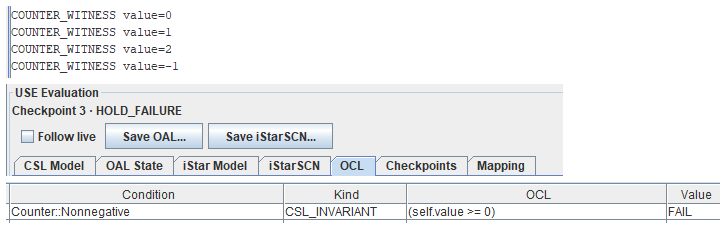
\includegraphics[width=5.76in,height=\textheight]{figures/fig-3-10.png}
\caption{Giá trị âm của Counter tại checkpoint.}\label{fig:3-10}
\end{figure}

\thesisfigure{fig:3-10} đối chiếu log và OCL trong phiên giữ âm 91765262 của TN07. Tại checkpoint 3, Counter vẫn có giá trị −1, bất biến Nonnegative cho kết quả FAIL và USE trả HOLD\_FAILURE. Đối chứng dùng một phiên riêng để kiểm tra điều gì xảy ra khi giá trị được sửa trong cùng nhóm plan.

\begin{figure}
\centering
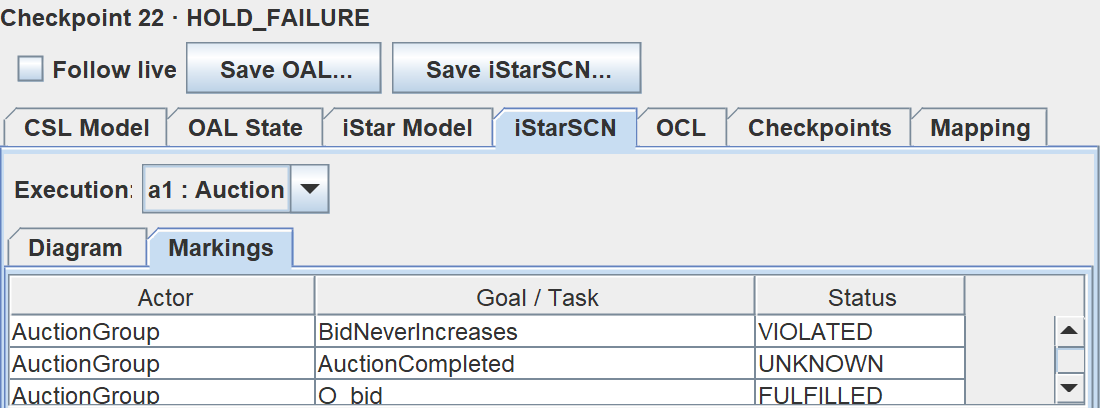
\includegraphics[width=5.76in,height=\textheight]{figures/fig-3-11.png}
\caption{Khôi phục giá trị Counter trước checkpoint.}\label{fig:3-11}
\end{figure}

Trong phiên khôi phục a17facf2 ở \thesisfigure{fig:3-11}, Console ghi bộ đếm lần lượt nhận −1 rồi 2. Tại checkpoint 3, Nonnegative cho kết quả PASS và USE trả APPROVE. Giá trị −1 chỉ xuất hiện trong log nguồn vì bộ đếm đã được khôi phục trước khi chụp ở cuối nhóm plan.

\subsection{Tái hiện kết quả khi đánh giá lại vết}\label{sec:3-5-3}

TN02 đánh giá lại cùng vết và cùng đặc tả của TN01. Quyết định và tập Goal/Task đã đạt khớp ở cả 58 checkpoint. Tại mốc 58, lần chạy gốc và lần đánh giá lại cùng ghi nhận AuctionCompleted cho hai phiên riêng biệt. Kết quả xác nhận khả năng tái hiện trên vết đã ghi. Một lần chạy mới có thể sinh vết khác nếu thứ tự thực thi của tác tử thay đổi.

\section{Giới hạn và hướng mở rộng}\label{sec:3-6}

Độ hạt checkpoint ảnh hưởng tới điểm phát hiện. TN03 phát hiện −1 ở cuối plan cha. Các giá trị 1 và 2 được tạo trong cùng nhóm plan con có thể không xuất hiện ở biên. Một hướng mở rộng là bổ sung điểm quan sát có chủ đích, xác định ảnh hưởng lên điều phối và đo chi phí trên các vết có thể so sánh.

Trong Auction, best\_bid cho biết giá đã được cải thiện và winner phản ánh nội dung thuộc tính được công bố. Để kiểm tra người thắng ứng với giá giữ lại, cần dữ liệu về chủ sở hữu của từng bid hoặc best-bidder và ràng buộc kiểm tra quan hệ đó. Việc xác nhận dịch vụ thực hiện đúng yêu cầu cũng cần ánh xạ Request/Scheme hoặc dữ liệu có ý nghĩa tương ứng. Các hướng này cần những ca đối chứng có thay đổi được xác định trước.

Bằng chứng thực nghiệm áp dụng cho workspace cục bộ, những thuộc tính và ràng buộc đã khai báo, cùng kết quả Goal, Task được đánh giá trên một kiểu ngữ cảnh trong mỗi đồ thị. Auction cho phép đối chiếu nhiều thể hiện cùng kiểu. TN04 và TN06 kiểm tra hai điểm khác nhau khi xử lý dữ liệu thiếu. Counter cô lập ảnh hưởng của ranh giới quan sát với một biến, qua đó TN07 xác định giới hạn lấy mẫu trong một tình huống cụ thể. Việc đánh giá lại chỉ bao phủ phần vết đã thu. Khả năng áp dụng cho hệ khác còn phụ thuộc vào cấu trúc tổ chức, dữ liệu được công bố và các luật ánh xạ cần khai báo. Một bước tiếp theo là chọn hệ đa tác tử có cấu trúc nhóm và loại thuộc tính khác Auction.

Để đối chiếu kết quả giữa hai công cụ, dữ kiện dùng làm mốc kiểm tra được lưu ở cả log nguồn và vết USE. Log bổ sung được đặt sau thao tác nguồn để xác nhận biến thể đã tạo đúng tình huống. Tuy nhiên, một số biến thể chủ động kiểm soát giá và lịch thao tác. Khi đọc kết quả, cần xét phiên bản runtime, phạm vi hook được theo dõi và việc một trường hợp có đúng điều kiện kích hoạt hay không. Kết quả theo từng ca chưa cung cấp số đo chi phí thời gian hay độ mở rộng. Những nhận định đó cần một nghiên cứu riêng có số lần lặp, tải và mốc đo xác định trước.

\section{Tổng kết chương}\label{sec:3-7}

TN01 cho thấy công cụ duy trì định danh, giá trị và lịch sử Goal/Task của từng phiên đấu giá. Khi đánh giá lại vết TN01, TN02 tái hiện quyết định và tập Goal/Task đã đạt ở cả 58 checkpoint. TN03 và TN05 xác nhận việc giữ dừng trước vi phạm đã quan sát, kể cả khi một Goal vi phạm trong lúc mọi bất biến đều đạt. TN04 và TN06 cho thấy công cụ phân biệt các trường hợp thiếu dữ liệu với vi phạm đã xác định.

TN07 cho thấy một thay đổi đã được khôi phục trước mốc quan sát có thể chỉ xuất hiện trong log nguồn. Phạm vi kết luận vì vậy phụ thuộc vào vị trí checkpoint và dữ liệu có trong đặc tả, chẳng hạn quan hệ giữa người thắng và giá được giữ trong Auction.

\chapter*{KẾT LUẬN}\label{ket-luan}
\addcontentsline{toc}{chapter}{KẾT LUẬN}

Nghiên cứu đã mở rộng công cụ USE để kiểm chứng khi thực thi đối với hệ thống xây dựng trên JaCaMo. Bài toán đặt ra là sử dụng dữ liệu quan sát được từ chương trình để kiểm tra cả tính hợp lệ của trạng thái lẫn tiến độ của mô hình mục tiêu. Phương pháp dùng CSL làm mô hình trạng thái chung. Phép chiếu có kiểu dựng đối tượng và liên kết trong USE từ ảnh chụp nguồn, đồng thời giữ định danh để mỗi đối tượng có lịch sử đánh giá riêng.

Trên trạng thái đã chiếu, bộ đánh giá OCL kiểm tra các bất biến và tính giá trị cho các điều kiện của Goal và Task. Lịch sử tiền điều kiện và hậu điều kiện giúp phân biệt một Task đang chờ bằng chứng với một Task đã đạt. Đối với Goal, cách cập nhật phụ thuộc vào loại mục tiêu và các quan hệ trong mô hình iStar. USE tổng hợp những kết quả này tại từng checkpoint và trả phản hồi cho JaCaMo. Việc gắn quyết định với đúng phiên và checkpoint giúp phân biệt trường hợp có vi phạm với trường hợp chưa đủ dữ liệu để kiểm chứng.

Các ca thực nghiệm lần lượt cung cấp bằng chứng về ba mặt. Trong TN01, hai phiên Auction dùng chung mô hình nhưng có hai đối tượng và hai lịch sử riêng. TN02 tái hiện quyết định và tập phần tử FULFILLED ở 58/58 checkpoint của cùng vết. Trong TN03 và TN04, hệ thống phân biệt giá trị vi phạm còn quan sát được ở cuối plan với trường hợp ảnh chụp báo thiếu. Các ca đối chứng bổ sung ở Chương 3 làm rõ điều kiện để phát hiện vi phạm Goal, xử lý một thuộc tính nguồn bị thiếu và ảnh hưởng của việc gom các plan con đồng bộ.

Kết quả có hiệu lực trong phạm vi những trạng thái và điều kiện đã quan sát. Một thay đổi xảy ra rồi được khôi phục trong cùng nhóm plan có thể xuất hiện trong log nguồn và vắng mặt ở snapshot. Tính hợp lệ của giá trị quan sát cũng phụ thuộc vào đặc tả. Ví dụ, để kiểm tra người thắng có thực sự là chủ của giá tốt nhất, cần dữ kiện liên kết người trả giá với giá được giữ. Kết quả replay trên một vết đã ghi cung cấp bằng chứng tái hiện cho vết đó.

Các hướng tiếp theo gồm mở rộng dữ kiện quan sát và thử nghiệm có kiểm soát với chính sách checkpoint ở những ranh giới khác nhau. Một hướng khác là đánh giá phương pháp trên hệ đa tác tử có cấu trúc tổ chức và mô hình dữ liệu khác Auction, đồng thời đo chi phí kiểm chứng qua nhiều lần chạy với cùng cấu hình.

\begin{thebibliography}{42}
\small\raggedright

\bibitem{ref-1}

M. Wooldridge và N. R. Jennings, ``Intelligent agents: Theory and practice,'' The Knowledge Engineering Review, vol.~10, no. 2, pp.~115--152, 1995. DOI: 10.1017/S0269888900008122.

\bibitem{ref-2}

O. Boissier, R. H. Bordini, J. F. Hübner, A. Ricci và A. Santi, ``Multi-agent oriented programming with JaCaMo,'' Science of Computer Programming, vol.~78, no. 6, pp.~747--761, 2013. DOI: 10.1016/j.scico.2011.10.004.

\bibitem{ref-3}

D. C. Schmidt, ``Guest editor's introduction: Model-driven engineering,'' Computer, vol.~39, no. 2, pp.~25--31, 2006. DOI: 10.1109/MC.2006.58.

\bibitem{ref-4}

M. Gogolla, F. Büttner và M. Richters, ``USE: A UML-based specification environment for validating UML and OCL,'' Science of Computer Programming, vol.~69, nos. 1--3, pp.~27--34, 2007. DOI: 10.1016/j.scico.2007.01.013. \href{https://github.com/useocl/use/blob/612df7cdcb290f9e3f39e36f42f773665338f71f/use-core/src/main/resources/examples/Documentation/HowToCheckUMLAndOCLModelsWithUSE/Gogolla_2007_SCP.pdf}{\ul{Bản PDF trong kho USE.}}

\bibitem{ref-5}

M. Leucker và C. Schallhart, ``A brief account of runtime verification,'' Journal of Logic and Algebraic Programming, vol.~78, no. 5, pp.~293--303, 2009. DOI: 10.1016/j.jlap.2008.08.004.

\bibitem{ref-6}

M. Mernik, J. Heering và A. M. Sloane, ``When and how to develop domain-specific languages,'' ACM Computing Surveys, vol.~37, no. 4, pp.~316--344, 2005. DOI: 10.1145/1118890.1118892.

\bibitem{ref-7}

T. Parr, S. Harwell và K. Fisher, ``Adaptive LL(*) parsing: The power of dynamic analysis,'' in Proceedings of the 2014 ACM International Conference on Object Oriented Programming Systems Languages \& Applications (OOPSLA), pp.~579--598, 2014. DOI: 10.1145/2660193.2660202.

\bibitem{ref-8}

R. H. Bordini và J. F. Hübner, ``BDI agent programming in AgentSpeak using Jason,'' in Computational Logic in Multi-Agent Systems (CLIMA 2005), Lecture Notes in Computer Science, vol.~3900, pp.~143--164, Springer, 2006. DOI: 10.1007/11750734\_9.

\bibitem{ref-9}

R. H. Bordini, J. F. Hübner và M. Wooldridge, Programming Multi-Agent Systems in AgentSpeak using Jason. Wiley, 2007. DOI: 10.1002/9780470061848.

\bibitem{ref-10}

A. Ricci, M. Piunti và M. Viroli, ``Environment programming in multi-agent systems: An artifact-based perspective,'' Autonomous Agents and Multi-Agent Systems, vol.~23, pp.~158--192, 2011. DOI: 10.1007/s10458-010-9140-7.

\bibitem{ref-11}

J. F. Hübner, J. S. Sichman và O. Boissier, ``Developing organised multiagent systems using the MOISE+ model: Programming issues at the system and agent levels,'' International Journal of Agent-Oriented Software Engineering, vol.~1, nos. 3/4, pp.~370--395, 2007. DOI: 10.1504/IJAOSE.2007.016266.

\bibitem{ref-12}

F. Dalpiaz, X. Franch và J. Horkoff, ``iStar 2.0 language guide,'' arXiv:1605.07767 {[}cs.SE{]}, 2016. \href{https://arxiv.org/abs/1605.07767}{\ul{Hướng dẫn iStar 2.0.}}

\bibitem{ref-13}

A. van Lamsweerde, ``Goal-oriented requirements engineering: A guided tour,'' in Proceedings of the Fifth IEEE International Symposium on Requirements Engineering, pp.~249--262, 2001. DOI: 10.1109/ISRE.2001.948567.

\bibitem{ref-14}

Object Management Group (OMG), OMG Unified Modeling Language (OMG UML), Version 2.5.1, 2017. https://www.omg.org/spec/UML/2.5.1. \href{https://github.com/Gavreg/UML-2.5.1-handbook/blob/acbcc0aef808826e2147334548f2f39c64c545ad/site/docs/omg-uml-2.5.1-formal-17-12-05.pdf}{\ul{Bản PDF đối chiếu.}}

\bibitem{ref-15}

Object Management Group (OMG), Object Constraint Language (OCL), Version 2.4, 2014. https://www.omg.org/spec/OCL/2.4.

\bibitem{ref-16}

M. Gogolla, J. Böhling và M. Richters, ``Validating UML and OCL models in USE by automatic snapshot generation,'' Software and Systems Modeling, vol.~4, no. 4, pp.~386--398, 2005. DOI: 10.1007/s10270-005-0089-y. \href{https://github.com/useocl/use/blob/612df7cdcb290f9e3f39e36f42f773665338f71f/use-core/src/main/resources/examples/Documentation/HowToCheckUMLAndOCLModelsWithUSE/Gogolla_2005_SOSYM.pdf}{\ul{Bản PDF trong kho USE.}}

\bibitem{ref-17}

F. Hilken và L. Hamann, ``History of the USE tool: 20 years of UML/OCL modeling made in Germany,'' Journal of Object Technology, vol.~19, no. 3, pp.~3:1--3:13, 2020. DOI: 10.5381/jot.2020.19.3.a20.

\bibitem{ref-18}

A. Bauer, M. Leucker và C. Schallhart, ``Runtime verification for LTL and TLTL,'' ACM Transactions on Software Engineering and Methodology, vol.~20, no. 4, Article 14, 2011. DOI: 10.1145/2000799.2000800.

\bibitem{ref-19}

R. H. Bordini, M. Fisher, W. Visser và M. Wooldridge, ``Verifying multi-agent programs by model checking,'' Autonomous Agents and Multi-Agent Systems, vol.~12, no. 2, pp.~239--256, 2006. DOI: 10.1007/s10458-006-5955-7.

\bibitem{ref-20}

A. Lomuscio, H. Qu và F. Raimondi, ``MCMAS: An open-source model checker for the verification of multi-agent systems,'' International Journal on Software Tools for Technology Transfer, vol.~19, pp.~9--30, 2017. DOI: 10.1007/s10009-015-0378-x.

\bibitem{ref-21}

K. M. Chandy và L. Lamport, ``Distributed snapshots: Determining global states of distributed systems,'' ACM Transactions on Computer Systems, vol.~3, no. 1, pp.~63--75, 1985. DOI: 10.1145/214451.214456.

\bibitem{ref-22}

R. H. Bordini, L. A. Dennis, B. Farwer và M. Fisher, ``Directions for agent model checking,'' in Specification and Verification of Multi-Agent Systems, pp.~103--123, Springer, 2010. DOI: 10.1007/978-1-4419-6984-2\_4.

\bibitem{ref-23}

R. Taleb, S. Hallé và R. Khoury, ``Uncertainty in runtime verification: A survey,'' Computer Science Review, vol.~50, Article 100594, 2023. DOI: 10.1016/j.cosrev.2023.100594.

\bibitem{ref-24}

D. C. Engelmann, A. Ferrando, A. R. Panisson, D. Ancona, R. H. Bordini và V. Mascardi, ``RV4JaCa---Towards Runtime Verification of Multi-Agent Systems and Robotic Applications,'' Robotics, vol.~12, no. 2, art. 49, 2023. DOI: 10.3390/robotics12020049.

\bibitem{ref-25}

A. Ferrando và V. Malvone, ``Towards the Combination of Model Checking and Runtime Verification on Multi-agent Systems,'' in Advances in Practical Applications of Agents, Multi-Agent Systems, and Complex Systems Simulation, LNCS 13616, pp.~140--152, Springer, 2022. DOI: 10.1007/978-3-031-18192-4\_12.

\bibitem{ref-26}

M. Fisher et al., ``Towards a framework for certification of reliable autonomous systems,'' Autonomous Agents and Multi-Agent Systems, vol.~35, art. 8, 2021. DOI: 10.1007/s10458-020-09487-2.

\bibitem{ref-27}

M. Fowler, Domain-Specific Languages. Addison-Wesley Professional, 2010. ISBN: 978-0-321-71294-3.

\bibitem{ref-28}

D.-Q. Nguyen, M.-P. Hoang, H.-H. Dao và D.-H. Dang, ``On Checking the Conformance between iStar and BPMN Models,'' bản PDF, 6 trang. \href{https://github.com/nguyentrungnghia1802/thesis/blob/b2b01b797c7acc8be209c8428c18f68518a502b6/1\%2C\%20Tham\%20Kh\%E1\%BA\%A3o/On\%20Checking\%20the\%20Conformance\%20between\%20iStar\%20and\%20BPMN_261012_173041_1.pdf}{\ul{Bản PDF đối chiếu.}}

\bibitem{ref-29}

R. H. Bordini, J. F. Hübner và D. M. Tralamazza, ``Using Jason to Implement a Team of Gold Miners,'' bản tác giả lưu trong kho dự án JaCaMo. \href{https://github.com/jacamo-lang/jacamo/blob/7699de3f2205943b8f2ac4f2edec0b47dba6eee3/doc/tutorials/gold-miners/initial-gold-miners/doc/cc-jason-lncs.pdf}{\ul{Bản PDF.}}

\bibitem{ref-30}

T. Parr, S. Harwell và K. Fisher, ``Adaptive LL(*) Parsing: The Power of Dynamic Analysis,'' báo cáo kỹ thuật, 24/03/2014. Bản dùng để trích Hình 1 và Hình 14. \href{https://github.com/antlr/website-antlr4/blob/052ec886db21c3367dc6fd2f304e1b5275988834/papers/allstar-techreport.pdf}{\ul{Bản PDF.}}

\bibitem{ref-31}

ANTLR Project, ANTLR 4 Documentation, các mục ``Lexer Rules'', ``Parser Rules'', ``Parse Tree Listeners'' và ``Tool Command Line Options''. \href{https://github.com/antlr/antlr4/tree/45be27daf036f79eced0e3e215fdfee78b4b38d2/doc}{\ul{Nguồn.}}

\bibitem{ref-32}

A. H. Bond và L. Gasser (biên tập), Readings in Distributed Artificial Intelligence. Morgan Kaufmann, 1988.

\bibitem{ref-33}

R. G. Smith, ``The Contract Net Protocol: High-Level Communication and Control in a Distributed Problem Solver,'' IEEE Transactions on Computers, vol.~C-29, no. 12, pp.~1104--1113, 1980. DOI: 10.1109/TC.1980.1675516.

\bibitem{ref-34}

G. Weiss (biên tập), Multiagent Systems: A Modern Approach to Distributed Artificial Intelligence. MIT Press, 1999. ISBN: 978-0-262-23203-6.

\bibitem{ref-35}

Foundation for Intelligent Physical Agents, FIPA Contract Net Interaction Protocol Specification, chuẩn SC00029H, 2002. \href{https://github.com/Rafael-Ramildes-Ferreira/Contract-Net-Protocol/blob/3348e5f8580b1924b1ec29422ae9106d7e1005ff/documentation/SC00029H.pdf}{\ul{Nguồn.}}

\bibitem{ref-36}

O. Boissier, R. H. Bordini, J. F. Hübner và A. Ricci, Multi-Agent Oriented Programming: Programming Multi-Agent Systems Using JaCaMo. MIT Press, 2020. Tài liệu và mã ví dụ kèm sách. \href{https://github.com/jacamo-lang/documentation/blob/85f564c7dd04353568efa267554aa0f4934d2de9/maop-book/readme.adoc}{\ul{Nguồn.}}

\bibitem{ref-37}

R. H. Bordini và J. F. Hübner, Jason: A Java-based interpreter for an extended version of AgentSpeak, release 0.9.5, Feb.~2007. \href{https://github.com/jason-lang/jason-lang.github.io/blob/6f9bbfd69bc5a6b737eddf8050c88e0289b07dba/doc/Jason.pdf}{\ul{Nguồn.}}

\bibitem{ref-38}

A. Ricci và A. Santi, CArtAgO and JaCa By Example. Università di Bologna, 2012, bản hướng dẫn cho CArtAgO 2.0.2 và Jason 1.3.4. \href{https://github.com/CArtAgO-lang/cartago/blob/440cd41c1810ceef6a627477c461776b3200236b/docs/cartago_by_examples/cartago_by_examples.pdf}{\ul{Nguồn.}}

\bibitem{ref-39}

O. Boissier, R. H. Bordini, J. F. Hübner và A. Ricci, Practical Session: Programming Multiagent Systems, tài liệu hướng dẫn thực hành WESAAC, 2013. \href{https://github.com/jacamo-lang/jacamo/blob/7699de3f2205943b8f2ac4f2edec0b47dba6eee3/doc/tutorials/house-building/slides-practical.pdf}{\ul{Nguồn.}}

\bibitem{ref-40}

J. F. Hübner, J. S. Sichman và O. Boissier, ``S-MOISE+: A Middleware for Developing Organised Multi-Agent Systems,'' trong Coordination, Organizations, Institutions, and Norms in Multi-Agent Systems, LNCS 3913, Springer, 2006, tr. 64--78. DOI: 10.1007/11775331\_5. \href{https://github.com/moise-lang/moise-lang.github.io/blob/707202c4dfb1b80b05b721ac2458041799abce15/doc/publications/Hubner-ooop2005.pdf}{\ul{Nguồn.}}

\bibitem{ref-41}

J. Pimentel và J. Castro, ``piStar Tool -- A Pluggable Online Tool for Goal Modeling,'' trong 2018 IEEE 26th International Requirements Engineering Conference, tr. 498--499, 2018. Tài liệu siêu mô hình và các ví dụ đi kèm trong kho piStar. \href{https://github.com/jhcp/piStar/tree/974d729ee9cbc193c93c403490ab2de471f591f0}{\ul{Nguồn.}} \href{https://github.com/jhcp/piStar/blob/974d729ee9cbc193c93c403490ab2de471f591f0/docs/METAMODEL.md}{\ul{Tài liệu siêu mô hình.}} \href{https://github.com/jhcp/piStar/blob/974d729ee9cbc193c93c403490ab2de471f591f0/tool/app/ui/istarmodels.js}{\ul{Tệp ví dụ.}}

\bibitem{ref-42}

I. Ayala, M. Amor, J. M. Horcas và L. Fuentes, ``A goal-driven software product line approach for evolving multi-agent systems in the Internet of Things,'' Knowledge-Based Systems, vol.~184, bài 104883, 2019. DOI 10.1016/j.knosys.2019.104883. Siêu mô hình iStar 2.0 đi kèm nghiên cứu. \href{https://github.com/jmhorcas/istar2fm/blob/48168790574308a08649df62c54f2fef872a30dd/metamodels/iStarMetamodel.ecore}{\ul{Nguồn.}}

\end{thebibliography}
\end{document}
